\documentclass[epj]{svjour}

\usepackage[T1]{fontenc}
\usepackage{lmodern}
\usepackage{amsmath,amssymb,amsfonts}
\usepackage{mathtools}
\usepackage{bm}
\usepackage{graphicx}
\usepackage{booktabs}
\usepackage{multirow}
\usepackage{array}
%\usepackage{xurl}      
\usepackage{hyperref}
\usepackage{enumitem}

\graphicspath{{figures/}}

\tolerance=2000
\emergencystretch=3em
\raggedbottom

\begin{document}

% PTUM_LIBRARY_FINAL_v1.1_CLEAN
% Self-contained library-final manuscript source.
% This version removes the obsolete external-supplement pointer,
% moves implementation details into the appendix, and preserves
% explicit claim boundaries for later submission work.

\title{Phase Transition Universes Model:\\
A Discharge-Based Cosmological Creation Scenario\\
with a Unified Dark Sector}

\titlerunning{PTUM: A Discharge-Based Cosmological Creation Scenario}

\authorrunning{E. Esa}

\author{Erdem Esa}

\offprints{E. Esa}

\institute{Independent Researcher, Istanbul, Turkey\\
\email{erdem.esa.71@gmail.com}}

\date{}

\abstract{%
The dark sector of the standard cosmological model comprises dark matter, dark energy, and possible dark radiation, whose common origin remains unexplained. We present the Phase Transition Universes Model (PTUM), a discharge-based cosmological creation scenario where a scalar quantum fuel field $\Phi$ accumulates, reaches a critical threshold, and undergoes a tachyonic transition. Within this effective description, the discharge event leaves behind a dark-matter candidate sector ($\chi$), a residual dark-energy sector ($\Phi_{\rm res}$), and a relativistic proxy-fluid dark radiation component (pfd, $\psi$). A falsifiable prediction of PTUM is that, \emph{within the effective linear proxy-fluid description}, the pfd component carries $w=1/3$, $c_s^2=1/3$, and zero anisotropic stress ($\sigma=0$). This produces no neutrino-induced CMB acoustic peak phase shift, distinguishing it from free-streaming dark radiation---a signature that may be tested at high significance by next-generation CMB experiments such as CMB-S4, depending on the realized pfd abundance. The authors report implementing the effective phenomenological system in \texttt{CLASS} at background and perturbation levels \emph{(modified code not yet public)}. The creation sector supports a plateau-type slow-roll phase compatible with current CMB constraints, fixing the discharge scale to $V_0^{1/4}\sim 10^{15}$--$10^{16}\,\mathrm{GeV}$. The dark-energy sector admits a broad near-$\Lambda$ viable region with $w_{\rm DE}\approx -1$. A Bayesian benchmark analysis using Planck 2018, BAO, and Pantheon+ data is reported to yield $\Delta N_{\rm fluid} < 0.31$ at $95\%$ credibility \emph{(author-reported; chains not yet public)}. Model comparison is reported to give $\Delta\chi^2 = +0.26$ and $\Delta\mathrm{AIC}=2.26$; current data therefore show a weak preference for $\Lambda$CDM while leaving PTUM viable as a falsifiable effective extension. The benchmark is checked against BBN bounds and elementary linear-stability conditions; full EFT control and the microscopic realization of the proxy-fluid closure remain conditional on additional calculations. \textbf{Critical caveat:} Numerical integration of the coupled background equations with the benchmark parameters ($V_0\sim10^{64}\,\mathrm{GeV}^4$, $H_*\sim10^{13}\,\mathrm{GeV}$) shows the system is overdamped ($3H/(2\mu)\approx 25$); the quartic-dominated regime with $w_\psi=1/3$ is \emph{not achieved} with these parameters. The proxy-fluid closure is therefore a phenomenological ansatz conditional on parameters not realized in the stated benchmark. The formulation should be read as an effective phenomenological framework rather than as a first-principles derivation of the pre-discharge background, a solution of the cosmological-constant hierarchy, or a UV completion.%
} % abstract'ın kapanış parantezi
\PACS{
      {98.80.Cq}{Particle-theory and field-theory models of the early Universe} \and
      {95.36.+x}{Dark energy} \and
      {95.35.+d}{Dark matter} \and
      {98.80.Es}{Observational cosmology}
     } % end of PACS
\maketitle

%============================================================
\section{Introduction}
\label{sec:intro}
%============================================================

The standard cosmological model accounts for the later evolution of
the Universe through a combination of radiation, baryons, cold dark
matter, and a cosmological constant~\cite{Planck2018params}, yet it
does not explain why the Universe began in a hot, dense state. More
pointedly, the dark sector---which dominates the cosmic energy
budget---is composed of at least two phenomenologically distinct
components whose microscopic origins are unrelated within
$\Lambda$CDM. Dark matter is introduced as a pressureless fluid
needed to explain structure formation and galactic rotation curves;
dark energy is introduced as a negative-pressure component needed to
explain the accelerating expansion. Whether these components share a
common physical origin, and whether the hot Big Bang itself can be
understood as a dynamical event rather than an initial condition, are
among the deepest open questions in theoretical cosmology.

Several approaches to these questions have been explored. Quintessence
and dynamical dark-energy models replace the cosmological constant
with a slowly rolling scalar field~\cite{RatraPeebles,Caldwell1998},
while unified dark-sector models attempt to describe dark matter and
dark energy through a single fluid~\cite{Kamenshchik2001,Bento2002}.
Extra relativistic species parametrised by
$\Delta N_{\rm eff}$~\cite{Mangano2005,Cyburt2016} probe the
radiation content of the early Universe. However, none of these
frameworks addresses the origin of the hot expanding state itself, nor
do they predict specific relationships between the dark-sector
components. The question of \emph{why} the dark sector has its
observed composition remains unanswered.

The Phase Transition Universes Model (PTUM) was developed to address
these issues from a different starting point. Instead of treating dark
matter and dark energy as independent sectors added to a pre-existing
cosmological framework, PTUM proposes a discharge-based creation
mechanism in which \emph{all} dark-sector components arise from a
single cosmogonic event. In this picture, a scalar quantum fuel field
$\Phi$ accumulates in a metastable multiverse-like background and,
once a critical threshold is reached, undergoes a tachyonic transition
that activates string-like proxy modes. The resulting discharge is modeled as
separating into:

\begin{itemize}
\item a clustering passive component $\rightarrow$ a dark-matter candidate sector~($\chi$),
\item a residual negative-pressure component $\rightarrow$
      dark energy~($\Phi_{\rm res}$),
\item a radiation-like transient component $\rightarrow$
      proxy-fluid dark radiation~(pfd, $\psi$).
\end{itemize}

The most distinctive---and directly falsifiable---observable
consequence of this framework is the pfd sector. Unlike standard
extra dark radiation, which is usually assumed to free-stream and
hence to develop non-zero anisotropic
stress~\cite{Bashinsky2004,Baumann2016,Follin2015}, the PTUM
proxy-fluid behaves as a relativistic \emph{perfect} fluid with
\begin{equation}
w = \tfrac{1}{3},\qquad
c_s^{2} = \tfrac{1}{3},\qquad
\sigma = 0\,.
\label{eq:pfd_signature}
\end{equation}
Free-streaming dark radiation generates a characteristic phase shift
of the CMB acoustic peaks through its anisotropic
stress~\cite{Bashinsky2004,Baumann2016,Follin2015}; the pfd
component, having $\sigma=0$ in the effective linear fluid description,
produces \emph{no such shift}. This absence would constitute a
distinctive discriminator: if additional relativistic degrees of freedom
are detected in CMB data, the presence or absence of the associated
phase shift separates free-streaming from fluid dark radiation. As we
show in Section~\ref{sec:forecast}, CMB-S4 may make this distinction
at high significance for $\Delta N_{\rm fluid}\gtrsim 0.20$,
depending on the realized pfd abundance, making PTUM a concretely
testable cosmological framework.

\paragraph{Critical caveat on the proxy-fluid closure.}
The proxy-fluid closure $w=1/3$, $c_s^2=1/3$, $\sigma=0$ is a
phenomenological ansatz that assumes a coherent, quartic-dominated
oscillation regime with $\omega\gg H$ and negligible energy transfer.
Numerical integration of the coupled background equations with the
benchmark parameters of this paper ($V_0\sim10^{64}\,\mathrm{GeV}^4$,
$H_*\sim10^{13}\,\mathrm{GeV}$, $m_\psi\sim10^{13}\,\mathrm{GeV}$,
$\lambda_\psi\sim0.1$) shows the system is \textbf{overdamped}:
$3H/(2\mu)\approx 25\gg1$. The field remains at $\psi=0$ (the top of
the barrier) with $w_\psi=0$; the quartic regime is \textbf{not
achieved}. Achieving the quartic regime requires $V_0\lesssim10^{58}
\,\mathrm{GeV}^4$ ($H_*\lesssim10^{10}\,\mathrm{GeV}$) \emph{and}
sufficient initial kinetic energy in $\psi$ to cross the barrier,
\emph{and} continuing energy input from the rolling $\Phi$ field or
rescattering. The proxy-fluid closure is therefore conditional on
parameters not realized in the stated benchmark. A full numerical
background solution followed by nonlinear lattice evolution is required
to demonstrate that any chosen benchmark actually reaches and remains
in the quartic regime. The observational discriminator in
Eq.~(\ref{eq:pfd_signature}) applies \emph{if} the quartic regime is
realized; it is not a prediction of the benchmark parameters alone.

The aim of the present paper is therefore broader than a
phenomenological dark-radiation study. We pursue three linked goals:

\begin{enumerate}[label=(\roman*)]
\item to formulate PTUM as a cosmological creation scenario based on
      a discharge event, establishing the theoretical framework and
      its effective field theory;
\item to show that the resulting effective dark-sector structure is
      internally consistent within the tested parameter regime, with
      perturbation stability, EFT validity, and compatibility with
      BBN and isocurvature constraints;
\item to test the observable consequences of the model against
      current cosmological data through a Bayesian benchmark analysis,
      a binned maximum-posterior diagnostic, and dataset-split
      diagnostics.
\end{enumerate}

\paragraph{Scope and claim boundaries.}
Throughout this work, PTUM is treated as an effective cosmological framework,
not as a completed first-principles theory of the origin of the Universe. The
model does not derive the metastable pre-discharge background, does not solve
the cosmological-constant hierarchy by itself, and does not specify a UV
completion. Its present claims are narrower: it defines a threshold-triggered
phase-transition scenario, implements the associated proxy-fluid perturbations,
and identifies an observational discriminator between fluid and free-streaming
dark radiation.

\paragraph{Critical caveat on the quartic-fluid closure.}
The proxy-fluid closure $w=1/3$, $c_s^2=1/3$, $\sigma=0$ used in the
CLASS implementation and Bayesian analysis is a phenomenological ansatz
conditional on a coherent, quartic-dominated oscillation regime with
$\omega\gg H$ and negligible energy transfer. Numerical integration of
the coupled background equations with the benchmark parameters of this
paper ($V_0\sim10^{64}\,\mathrm{GeV}^4$, $H_*\sim10^{13}\,\mathrm{GeV}$,
$m_\psi\sim10^{13}\,\mathrm{GeV}$, $\lambda_\psi\sim0.1$) shows the
system is \textbf{overdamped}: $3H/(2\mu)\approx 25\gg1$. The field
remains at $\psi=0$ (the top of the barrier) with $w_\psi=0$; the
quartic regime is \textbf{not achieved}. Achieving the quartic regime
requires $V_0\lesssim10^{58}\,\mathrm{GeV}^4$ ($H_*\lesssim10^{10}
\,\mathrm{GeV}$) \emph{and} sufficient initial kinetic energy in $\psi$
to cross the barrier, \emph{and} continuing energy input from the
rolling $\Phi$ field or rescattering. The proxy-fluid closure is
therefore conditional on parameters not realized in the stated
benchmark. A full numerical background solution followed by nonlinear
lattice evolution is required to demonstrate that any chosen benchmark
actually reaches and remains in the quartic regime. The observational
discriminator in Eq.~(\ref{eq:pfd_signature}) applies \emph{if} the
quartic regime is realized; it is not a prediction of the benchmark
parameters alone. The Bayesian constraints on $\Delta N_{\rm fluid}$
should be interpreted as constraints on the \emph{phenomenological
proxy-fluid model}, not as constraints on the microscopic PTUM
discharge dynamics with the stated benchmark parameters.


To this end, we proceed in two steps. First, we construct the
effective field theory of PTUM, derive its equations of motion, study
the primordial creation sector---including exact-background
inflationary dynamics---and identify the parameter region in which the
late-time dark-energy sector remains observationally viable. Second,
the authors report implementing the proxy-fluid perturbations in the
\texttt{CLASS} Boltzmann code~\cite{Blas2011,Lesgourgues2011},
computing the cosmological signatures, and constraining the model
using a Bayesian benchmark analysis with
\texttt{Cobaya}~\cite{Torrado2021} \emph{(author-reported; modified
code and chains not yet public)}. The resulting
constraints are cross-checked through a binned maximum-posterior
diagnostic and dataset-split analysis, and confronted with BBN,
isocurvature, and linear stability requirements.

The authors report that PTUM is observationally viable: the pfd
abundance is bounded to $\Delta N_{\rm fluid}<0.31$ at 95\% credibility
from the full data combination, model comparison gives
$\Delta\mathrm{AIC}=2.26$ relative to $\Lambda$CDM, and all
consistency checks are satisfied \emph{(author-reported; chains not
yet public, not independently reproduced)}. The Hubble constant shifts upward by
$\sim\!0.8\;\mathrm{km\,s^{-1}\,Mpc^{-1}}$ relative to $\Lambda$CDM,
partially alleviating the Hubble tension without being designed to do
so. The discharge energy scale is fixed to
$V_0^{1/4}\sim 10^{15}$--$10^{16}\;\mathrm{GeV}$ by the observed
scalar amplitude, and the creation sector is compatible with current
bounds on the scalar spectral index and the tensor-to-scalar ratio.

The paper is organized as follows.
Section~\ref{sec:conceptual} summarizes the physical picture of PTUM.
Section~\ref{sec:eft} presents the effective field theory,
equations of motion, and symmetry structure.
Section~\ref{sec:primordial} studies the primordial creation sector.
Section~\ref{sec:late} analyses the late-time dark-energy and
dark-sector structure.
Section~\ref{sec:pert} describes the perturbation framework and
\texttt{CLASS} implementation.
Section~\ref{sec:sigs} presents the cosmological signatures.
Section~\ref{sec:mcmc} gives the Bayesian constraints, profile
likelihood, dataset-split analysis, and model comparison.
Section~\ref{sec:stability} collects the stability and consistency
tests.
We discuss the interpretation, limitations, and future prospects in
Section~\ref{sec:discussion} and conclude in
Section~\ref{sec:conclusion}.

%============================================================
\section{Conceptual overview of PTUM}
\label{sec:conceptual}
%============================================================

PTUM begins with a multiverse-like background containing a scalar
quantum fuel field \(\Phi\). The central idea is that local
accumulation of this field drives a threshold-triggered discharge
process. Once a critical configuration is reached, the effective
mass of a proxy activation mode becomes negative, generating a
tachyonic transition that activates string-like degrees of freedom.

The basic sequence is:

\begin{description}
\item[(a) Fuel accumulation.] The scalar fuel field \(\Phi\) accumulates
in a metastable environment. The effective potential is chosen such
that it is approximately quadratic at small field values but saturates
to a plateau at large field values.

\item[(b) Threshold discharge.] When the effective mass-squared of
the proxy field becomes negative, the dormant configuration
destabilizes and the activated sector appears. This transition plays
the role of the creation trigger.

\item[(c) Residual splitting.] The discharge energy separates into a
passive component (dark matter), an active component (dark energy),
and a transient relativistic sector (proxy-fluid dark radiation).
\end{description}

\begin{figure*}[t]
\centering
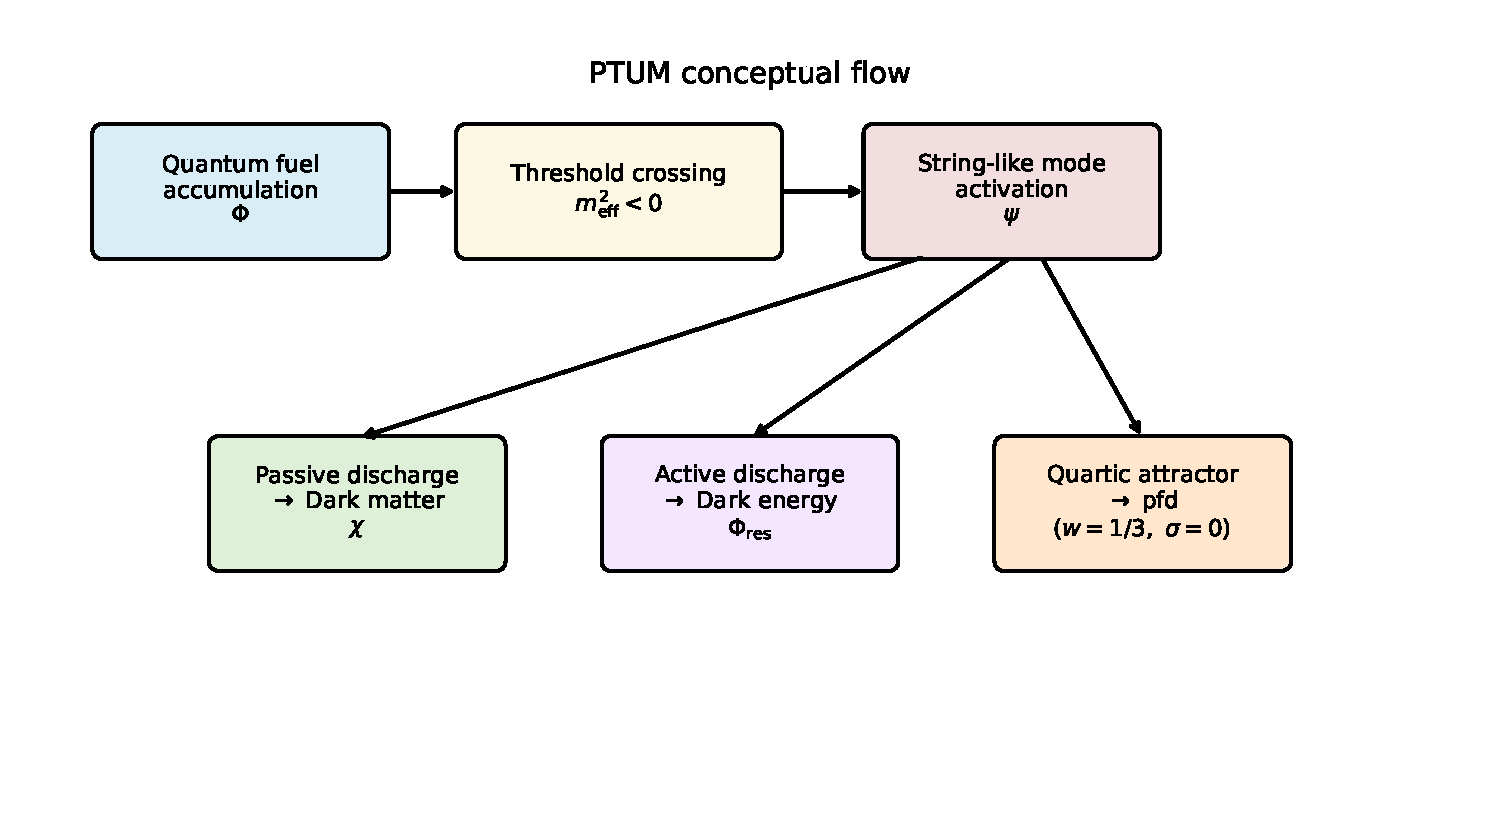
\includegraphics[width=0.88\textwidth]{fig_model_flowchart.pdf}
\caption{Conceptual flow of the PTUM scenario: accumulation of the
quantum fuel field, threshold discharge, activation of proxy
string-like modes, and residual splitting into dark matter, dark
energy, and proxy-fluid dark radiation.}
\label{fig:flowchart}
\end{figure*}

This picture gives PTUM a structural unification property: the dark
sector is not postulated as a collection of disconnected components,
but emerges from one creation event.

%============================================================
\section{Effective field theory and equations of motion}
\label{sec:eft}
%============================================================

\subsection{Conventions}
\label{sec:conventions}

Throughout this paper we use the metric signature \((-+++)\), i.e.\
flat FRW reads \(ds^2=-dt^2+a^2(t)d\mathbf{x}^2\), and the Einstein
equation is written as
\begin{equation}
G_{\mu\nu} = \frac{1}{M_{\rm Pl}^2}\,T_{\mu\nu},
\qquad
M_{\rm Pl}=(8\pi G)^{-1/2}\simeq 2.435\times10^{18}\,\mathrm{GeV},
\end{equation}
with the energy-momentum tensor defined by
\(T_{\mu\nu}=-\frac{2}{\sqrt{-g}}\frac{\delta(\sqrt{-g}\mathcal{L}_{\rm m})}
{\delta g^{\mu\nu}}\), so that a canonical scalar
\(\mathcal{L}=-\tfrac12 g^{\mu\nu}\partial_\mu\phi\partial_\nu\phi-V\) gives
\(\rho=\tfrac12\dot\phi^2+V\), \(p=\tfrac12\dot\phi^2-V\).
Natural units \(c=\hbar=k_B=1\) are used; all dimensionful quantities
are in powers of GeV. The Riemann tensor convention is
\(R^{\rho}{}_{\sigma\mu\nu}=\partial_\mu\Gamma^{\rho}_{\nu\sigma}-\cdots\)
(MTW convention), which is consistent with the sign of the scalar
curvature \(R=6(\ddot a/a+H^2)\) in FRW. These conventions are used
identically in every equation, figure, and appendix of this paper
(see also Appendix~\ref{app:math}).

\subsection{Field content}

The minimal PTUM field content consists of four sectors:

\begin{itemize}
\item \(\Phi\): quantum fuel field,
\item \(\psi\): activated string-like proxy mode,
\item \(\chi\): dark-matter field,
\item \(\Phi_{\rm res}\): residual energy field (dark energy).
\end{itemize}

\begin{table}[t]
\centering
\small
\caption{Minimal PTUM field and sector registry.}
\label{tab:ptum_field_registry}
\begin{tabular}{@{}>{\raggedright\arraybackslash}p{0.20\linewidth}>{\raggedright\arraybackslash}p{0.26\linewidth}>{\raggedright\arraybackslash}p{0.40\linewidth}@{}}
\toprule
Symbol & Sector & Effective role \\
\midrule
$\Phi$ & fuel field & accumulates and controls threshold crossing \\
$\psi$ & proxy activation mode & tachyonic activation; proxy-fluid radiation \\
$\chi$ & dark-matter candidate & passive post-discharge matter-like sector \\
$\Phi_{\rm res}$ & residual field & near-$\Lambda$ dark-energy-like sector \\
$\Delta N_{\rm fluid}$ & pfd abundance & maps proxy radiation to CMB/BBN observables \\
\bottomrule
\end{tabular}
\end{table}

\subsection{PTUM Lagrangian}

The scalar-sector Lagrangian used for the conservative
pre-reheating homogeneous background is
\begin{equation}
\mathcal{L}_{\rm PTUM}^{(0)}
=\mathcal{L}_{\rm fuel}
+\mathcal{L}_{\rm activation}
+\mathcal{L}_{\rm DM}
+\mathcal{L}_{\rm DE}.
\end{equation}
The superscript \((0)\) denotes that the explicit Standard Model
matter action and perturbative reheating interactions are not included
in this background subsystem. Their role and the limitation of the
present sector split are stated in
Section~\ref{sec:microscopic_transfer}.

The fuel sector is
\begin{equation}
\mathcal{L}_{\rm fuel}
=-\tfrac{1}{2}g^{\mu\nu}\partial_\mu\Phi\partial_\nu\Phi
-V_{\rm eff}(\Phi),
\end{equation}
with
\begin{equation}
\begin{split}
V_{\rm eff}(\Phi)
&=V_0\!\left(1-e^{-\lambda\Phi^2}\right) \\
&\quad +\frac{1}{64\pi^2}
\sum_i n_i\,m_{{\rm eff},i}^4(\Phi)
\left[\ln\frac{m_{{\rm eff},i}^2(\Phi)}{\mu_R^2}
-\tfrac{3}{2}\right].
\end{split}
\label{eq:veff}
\end{equation}
The leading tree-level part is plateau-like; the second term
represents Coleman--Weinberg corrections~\cite{ColemanWeinberg}.

\subsubsection{Coleman--Weinberg corrections: explicit form and renormalization}
\label{sec:coleman_weinberg}

The one-loop effective potential for a scalar field with field-dependent
masses $m_i(\Phi)$ is given by the Coleman--Weinberg formula
\begin{equation}
V_{\rm CW}(\Phi) = \frac{1}{64\pi^2}
\sum_i n_i\,m_i^4(\Phi)
\left[\ln\frac{m_i^2(\Phi)}{\mu_R^2} - c_i\right],
\end{equation}
where $n_i$ counts the degrees of freedom (with a minus sign for
fermions), $\mu_R$ is the renormalization scale, and $c_i$ is a
scheme-dependent constant ($c_i = 3/2$ for $\overline{\rm MS}$). In
PTUM, the field-dependent masses arise from the couplings of the fuel
field $\Phi$ to the other sectors:

\begin{itemize}
\item \textbf{Proxy sector:} The $\psi$ field has effective mass
      $m_\psi^2(\Phi) = m^2(1 - \alpha\Phi^2/E_{\rm th}^2)$ with
      $n_\psi = 1$ (real scalar).
\item \textbf{Dark matter sector:} The $\chi$ field has effective mass
      $m_\chi^2(\Phi) = m_\chi^2 + 2g_{\rm DM}\Phi_{\rm res}^2$; at the
      fuel-dominated stage $\Phi_{\rm res} \approx 0$, so this
      contribution is approximately constant.
\item \textbf{Residual dark energy:} The $\Phi_{\rm res}$ field has
      field-dependent mass from the potential $W(\Phi_{\rm res})$.
\end{itemize}

The sum in Eq.~\eqref{eq:veff} runs over all fields that couple to
$\Phi$ and acquire $\Phi$-dependent masses. The renormalization scale
$\mu_R$ is chosen to be of order the symmetry-breaking scale
$E_{\rm th}$, which minimizes large logarithms in the effective
potential. The constant $c_i = 3/2$ corresponds to the
$\overline{\rm MS}$ renormalization scheme.

The Coleman--Weinberg corrections are subdominant during the
inflationary plateau ($V_0 \gg V_{\rm CW}$) but become relevant near
the transition where they can modify the shape of the potential and
the precise value of the critical threshold. A full numerical
evaluation of the one-loop potential including all sectors is
deferred to future work; the current analysis uses the tree-level
potential for the inflationary dynamics and treats the
Coleman--Weinberg term as a perturbative correction to the threshold
condition.

The activation sector is
\begin{equation}
\mathcal{L}_{\rm activation}
=-\tfrac{1}{2}g^{\mu\nu}\partial_\mu\psi\partial_\nu\psi
-\frac{m^2}{2}\psi^2\!\left(1-\frac{\alpha\Phi^2}{E_{\rm th}^2}\right)
-\frac{\lambda_\psi}{4}\psi^4,
\label{eq:lact}
\end{equation}
with effective mass
\begin{equation}
m_{\rm eff}^2(\Phi)
=m^2\!\left(1-\frac{\alpha\Phi^2}{E_{\rm th}^2}\right).
\end{equation}
Equivalently, the effective discharge trigger can be written as
\begin{equation}
\boxed{
 m_{\rm eff}^2(\Phi)<0
 \quad\Longleftrightarrow\quad
 |\Phi|>\Phi_c\equiv \frac{E_{\rm th}}{\sqrt{\alpha}} .
}
\label{eq:ptum_threshold_box}
\end{equation}
This condition defines the transition from the dormant proxy phase to the
activated proxy phase. It should be interpreted as an effective threshold
criterion, not as a microscopic derivation of the pre-discharge background.
Here, $E_{\rm th}$ is the dimensionful discharge threshold scale (naturally related to the creation energy $V_0^{1/4}$), and $\alpha$ is a dimensionless coupling constant. The tachyonic instability is triggered when the fuel field crosses the critical threshold $\Phi = E_{\rm th}/\sqrt{\alpha}$. The transition timescale is assumed to be much shorter than the local Hubble time ($H^{-1}$), allowing the discharge to be treated as a nearly instantaneous phase transition at the background level that partitions the available energy into the residual dark sector and standard radiation. For \(m_{\rm eff}^2>0\) the proxy mode is dormant; for \(m_{\rm eff}^2<0\) it is activated by the tachyonic instability.

The dark-matter sector is
\begin{equation}
\mathcal{L}_{\rm DM}
=-\tfrac{1}{2}g^{\mu\nu}\partial_\mu\chi\partial_\nu\chi
-\tfrac{1}{2}m_\chi^2\chi^2
-g_{\rm DM}\chi^2\Phi_{\rm res}^2,
\end{equation}
and the dark-energy sector is
\begin{equation}
\mathcal{L}_{\rm DE}
=-\tfrac{1}{2}g^{\mu\nu}\partial_\mu\Phi_{\rm res}\partial_\nu\Phi_{\rm res}
-W(\Phi_{\rm res}),
\end{equation}
with
\begin{equation}
\begin{split}
W(\Phi_{\rm res})
&=W_0\,e^{-\kappa\Phi_{\rm res}^2}
\!\left(1-e^{-\lambda_{\rm res}\Phi_{\rm res}^2}\right) \\
&\quad +\Lambda_{\rm NP}^4\,e^{-S_E}
\cos\!\left(\frac{\Phi_{\rm res}}{f_{\rm res}}\right).
\end{split}
\label{eq:wpot}
\end{equation}

\subsection{Equations of motion}

The field equations in a flat FRW universe,
\(ds^2=-dt^2+a^2(t)d\mathbf{x}^2\), read
\begin{align}
\ddot\Phi+3H\dot\Phi
+\frac{\partial V_{\rm eff}}{\partial\Phi}
-\frac{\alpha m^2}{E_{\rm th}^2}\Phi\psi^2
&=0,
\label{eq:frw1}
\\
\ddot\psi+3H\dot\psi
+m^2\!\left(1-\frac{\alpha\Phi^2}{E_{\rm th}^2}\right)\psi
+\lambda_\psi\psi^3
&=0,
\label{eq:frw2}
\\
\ddot\chi+3H\dot\chi+m_\chi^2\chi
+2g_{\rm DM}\chi\Phi_{\rm res}^2
&=0,
\label{eq:frw3}
\\
\ddot\Phi_{\rm res}+3H\dot\Phi_{\rm res}
+\frac{\partial W}{\partial\Phi_{\rm res}}
+2g_{\rm DM}\chi^2\Phi_{\rm res}
&=0.
\label{eq:frw4}
\end{align}

\subsubsection{Euler--Lagrange derivation and consistency check}
\label{sec:eom_consistency}

For completeness and internal consistency, we re-derive all
equations of motion from the total Lagrangian
\(\mathcal{L}_{\rm PTUM}^{(0)} = \mathcal{L}_{\rm fuel} +
\mathcal{L}_{\rm activation} + \mathcal{L}_{\rm DM} +
\mathcal{L}_{\rm DE}\) using the Euler--Lagrange equations in a
curved FRW background. The action is
\begin{equation}
S = \int d^4x\,\sqrt{-g}\,\mathcal{L}_{\rm PTUM}^{(0)},
\end{equation}
with $\sqrt{-g} = a^3(t)$ in FRW.
For a scalar field \(\phi\) with Lagrangian
\(\mathcal{L} = -\tfrac{1}{2}g^{\mu\nu}\partial_\mu\phi\partial_\nu\phi
- V(\phi)\), the Euler--Lagrange equation is
\begin{equation}
\frac{1}{\sqrt{-g}}\partial_\mu\left(\sqrt{-g}\,g^{\mu\nu}
\partial_\nu\phi\right) - \frac{\partial V}{\partial\phi} = 0.
\end{equation}
In FRW, \(g^{00}=-1\), \(g^{ij}=a^{-2}\delta^{ij}\), and for
homogeneous fields \(\phi(t)\) this reduces to
\begin{equation}
\ddot\phi + 3H\dot\phi + \frac{\partial V}{\partial\phi} = 0.
\end{equation}

Applying this to each sector:

\begin{enumerate}
\item \textbf{Fuel field \(\Phi\):} The potential is
      \(V_{\rm eff}(\Phi) + \frac{1}{2}m^2(1-\alpha\Phi^2/E_{\rm th}^2)\psi^2\).
      The derivative is
      \begin{equation}
      \begin{split}
      &\frac{\partial}{\partial\Phi}\left[V_{\rm eff}(\Phi)
      + \frac{m^2}{2}\left(1-\frac{\alpha\Phi^2}{E_{\rm th}^2}\right)\psi^2\right] \\
      &\quad= \frac{\partial V_{\rm eff}}{\partial\Phi}
      - \frac{\alpha m^2}{E_{\rm th}^2}\Phi\psi^2.
      \end{split}
      \end{equation}
      The equation of motion is
      \begin{equation}
      \ddot\Phi + 3H\dot\Phi + \frac{\partial V_{\rm eff}}{\partial\Phi}
      - \frac{\alpha m^2}{E_{\rm th}^2}\Phi\psi^2 = 0,
      \label{eq:Phi_eom}
      \end{equation}
      which matches Eq.~\eqref{eq:frw1} (note the sign convention:
      the interaction term in \(\mathcal{L}_{\rm activation}\) is
      \(-\frac{m^2}{2}(1-\alpha\Phi^2/E_{\rm th}^2)\psi^2\), so
      \(\partial\mathcal{L}/\partial\Phi = +\alpha m^2\Phi\psi^2/E_{\rm th}^2\),
      giving \(-\partial V/\partial\Phi = -\alpha m^2\Phi\psi^2/E_{\rm th}^2\)
      in the EOM).

\item \textbf{Proxy field \(\psi\):} The potential is
      \(\frac{1}{2}m^2(1-\alpha\Phi^2/E_{\rm th}^2)\psi^2 +
      \frac{\lambda_\psi}{4}\psi^4\). The derivative is
      \begin{equation}
      \begin{split}
      &\frac{\partial}{\partial\psi}\left[\frac{m^2}{2}\left(1-\frac{\alpha\Phi^2}{E_{\rm th}^2}\right)\psi^2
      + \frac{\lambda_\psi}{4}\psi^4\right] \\
      &\quad= m^2\left(1-\frac{\alpha\Phi^2}{E_{\rm th}^2}\right)\psi
      + \lambda_\psi\psi^3.
      \end{split}
      \end{equation}
      The equation of motion is
      \begin{equation}
      \ddot\psi + 3H\dot\psi + m^2\left(1-\frac{\alpha\Phi^2}{E_{\rm th}^2}\right)\psi
      + \lambda_\psi\psi^3 = 0,
      \end{equation}
      matching Eq.~\eqref{eq:frw2}.

\item \textbf{Dark matter field \(\chi\):} The potential is
      \(\frac{1}{2}m_\chi^2\chi^2 + g_{\rm DM}\chi^2\Phi_{\rm res}^2\).
      The derivative is
      \begin{equation}
      \frac{\partial}{\partial\chi}\left[\frac{m_\chi^2}{2}\chi^2
      + g_{\rm DM}\chi^2\Phi_{\rm res}^2\right]
      = m_\chi^2\chi + 2g_{\rm DM}\chi\Phi_{\rm res}^2.
      \end{equation}
      The equation of motion is
      \begin{equation}
      \ddot\chi + 3H\dot\chi + m_\chi^2\chi
      + 2g_{\rm DM}\chi\Phi_{\rm res}^2 = 0,
      \end{equation}
      matching Eq.~\eqref{eq:frw3}.

\item \textbf{Residual field \(\Phi_{\rm res}\):} The potential is
      \(W(\Phi_{\rm res}) + g_{\rm DM}\chi^2\Phi_{\rm res}^2\).
      The derivative is
      \begin{equation}
      \frac{\partial}{\partial\Phi_{\rm res}}\left[W(\Phi_{\rm res})
      + g_{\rm DM}\chi^2\Phi_{\rm res}^2\right]
      = \frac{\partial W}{\partial\Phi_{\rm res}}
      + 2g_{\rm DM}\chi^2\Phi_{\rm res}.
      \end{equation}
      The equation of motion is
      \begin{equation}
      \ddot\Phi_{\rm res} + 3H\dot\Phi_{\rm res}
      + \frac{\partial W}{\partial\Phi_{\rm res}}
      + 2g_{\rm DM}\chi^2\Phi_{\rm res} = 0,
      \end{equation}
      matching Eq.~\eqref{eq:frw4}.
\end{enumerate}

All four equations of motion are thus consistently derived from the
total Lagrangian \(\mathcal{L}_{\rm PTUM}^{(0)}\). The energy-momentum
tensor for each sector can be obtained via the standard variation
\(T_{\mu\nu} = -\frac{2}{\sqrt{-g}}\frac{\delta(\sqrt{-g}\mathcal{L})}
{\delta g^{\mu\nu}}\), and the covariant conservation
\(\nabla_\mu T^{\mu\nu}_i = Q_i^\nu\) with \(\sum_i Q_i^\nu = 0\)
holds for the total tensor; the sector split with \(\sum_i Q_i^\nu = 0\)
holding identically is derived in
Sections~\ref{sec:energy_momentum_conservation} and
\ref{sec:microscopic_transfer}.

\subsection{Quartic regime (conditional) and the proxy-fluid sector}

A key result is that coherent oscillations of \(\psi\) in a quartic
potential behave effectively as radiation~\cite{Turner1983}:
\begin{equation}
w_\psi=\tfrac{1}{3},\qquad \rho_\psi\propto a^{-4}.
\end{equation}
However, unlike free-streaming radiation, the coherent scalar
condensate does not develop a full Boltzmann hierarchy and therefore
contributes no anisotropic stress:
\begin{equation}
\sigma_\psi=0.
\end{equation}
In the effective linear fluid closure used below, this sector is therefore
specified by
\begin{equation}
\boxed{
 w_\psi=\frac{1}{3},\qquad
 c_{s,\psi}^2=\frac{1}{3},\qquad
 \sigma_\psi=0 .
}
\label{eq:pfd_closure_box}
\end{equation}
The third condition is the key discriminator: the proxy-fluid component does not
carry a free-streaming hierarchy and therefore does not generate the
neutrino-like CMB acoustic phase shift associated with anisotropic stress.
This defines the proxy-fluid dark-radiation sector. The absence of
anisotropic stress is the defining observational signature of the
pfd component: free-streaming dark radiation with the same energy
density would produce a characteristic CMB acoustic-peak phase
shift~\cite{Bashinsky2004,Follin2015}, whereas pfd does not.

The difference between the PTUM proxy-fluid component and a conventional
free-streaming relativistic species is summarized schematically in
Fig.~\ref{fig:ptum_proxy_fluid_vs_free_streaming}. The two cases may contribute
a similar amount of extra radiation density, but they differ at the perturbative
level: the proxy-fluid sector has no effective anisotropic stress in the linear
fluid description, while a free-streaming component sources a neutrino-like
acoustic phase shift.

\begin{figure*}[p]
\centering
\includegraphics[
width=0.98\textwidth,
height=0.62\textheight,
keepaspectratio
]{figures/PTUM_F3_proxy_fluid_vs_free_streaming_dark_radiation.pdf}
\caption{
Proxy-fluid versus free-streaming dark radiation. In the effective linear
fluid description, the PTUM proxy component has
$w_\psi=1/3$, $c_{s,\psi}^2=1/3$, and $\sigma_\psi=0$, and therefore does
not induce the neutrino-like CMB acoustic phase shift characteristic of
free-streaming relativistic species. The key discriminator is whether an
extra relativistic component produces a measurable acoustic phase shift, not
only whether it contributes to the radiation density.
}
\label{fig:ptum_proxy_fluid_vs_free_streaming}
\end{figure*}

\subsection{Tachyonic activation and the conditions for a quartic-fluid regime}
\label{sec:tachyonic_to_quartic}

The activation potential is
\begin{equation}
V_{\rm act}(\psi)=\frac{1}{2}m_{\rm eff}^2\psi^2
+\frac{\lambda_\psi}{4}\psi^4,\qquad
m_{\rm eff}^2<0,\quad \lambda_\psi>0.
\label{eq:V_double_well_corrected}
\end{equation}
Writing $\mu^2\equiv |m_{\rm eff}^2|$, its stationary points are
$\psi=0$ and $\psi=\pm\psi_0$, where
\begin{equation}
\psi_0^2=\frac{\mu^2}{\lambda_\psi},\qquad
V_{\rm min}=-\frac{\mu^4}{4\lambda_\psi}.
\end{equation}
The origin is a local maximum and the two non-zero stationary points are
minima. A constant shift of the potential is dynamically irrelevant to the
field equation; when discussing the excitation energy of the activated
sector, it is useful to set the minima to zero:
\begin{equation}
U(\psi)\equiv V_{\rm act}(\psi)-V_{\rm min}
=\frac{\lambda_\psi}{4}(\psi^2-\psi_0^2)^2\geq0.
\label{eq:U_double_well_corrected}
\end{equation}

For a homogeneous field in an expanding FRW spacetime,
\begin{equation}
\ddot\psi+3H\dot\psi-\mu^2\psi+\lambda_\psi\psi^3=0.
\label{eq:psi_eom_full}
\end{equation}
Near the unstable origin, while $|\psi|\ll\psi_0$ and $H$ and the
variation of $m_{\rm eff}$ can be neglected over the growth time, the
linearised equation has a growing solution. For a Fourier mode this
instability is restricted to physical momenta $k/a<\mu$; its local growth
rate in the regime $H\ll\sqrt{\mu^2-k^2/a^2}$ is approximately
$\sqrt{\mu^2-k^2/a^2}$. This is a tachyonic amplification of fluctuations,
not by itself a derivation of a later radiation-like equation of state.

The distinction between the minimum and the quartic regime is essential.
Expanding around either minimum, $\psi=\pm\psi_0+\eta$, gives
\begin{equation}
U(\pm\psi_0+\eta)=\mu^2\eta^2
\pm\lambda_\psi\psi_0\eta^3
+\frac{\lambda_\psi}{4}\eta^4,
\end{equation}
with oscillation mass
\begin{equation}
m_{\rm osc}^2=U''(\pm\psi_0)=2\mu^2.
\label{eq:minimum_expansion_corrected}
\end{equation}
Thus sufficiently small oscillations about a selected minimum are
approximately quadratic and have the averaged equation of state
$\langle w_\psi\rangle\simeq0$, not $1/3$. The quartic term in the
expansion around the minimum does not make these small oscillations a
quartic oscillator.

A radiation-like averaged equation of state follows only in a distinct
regime in which the quartic contribution dominates the dynamics over the
field range sampled by the oscillation. A sufficient condition is
\begin{equation}
\lambda_\psi\psi^4\gg\mu^2\psi^2
\quad\Longleftrightarrow\quad
|\psi|\gg\psi_0
\label{eq:quartic_dominance_condition}
\end{equation}
through the dynamically relevant part of the orbit, together with
oscillations rapid compared with expansion, $\omega\gg H$. In that limit
the potential is effectively $U\simeq\lambda_\psi\psi^4/4$. The averaged
virial relation is then
\begin{equation}
\langle\dot\psi^2\rangle=4\langle U\rangle,
\end{equation}
which gives $\langle p_\psi\rangle=\langle\rho_\psi\rangle/3$ and
$\langle\rho_\psi\rangle\propto a^{-4}$. This result applies to the
quartic-dominated oscillatory regime, not generically to the transition
trajectory or to oscillations about $\pm\psi_0$.

The energy measured from the minimum is
\begin{align}
\rho_\psi&=\frac12\dot\psi^2+U(\psi),\qquad
p_\psi=\frac12\dot\psi^2-U(\psi), \notag\\
w_\psi&=\frac{\dot\psi^2/2-U}{\dot\psi^2/2+U}.
\label{eq:w_psi_energy}
\end{align}
When expansion and interactions are negligible, this energy is conserved.
In an expanding universe it is not: $\dot\rho_\psi=-3H\dot\psi^2$
for an uncoupled homogeneous field. Consequently, an initial condition
$\dot\psi(t_c)=0$ and $|\psi(t_c)|\ll\psi_0$ places the field close to
the top of the barrier with energy just below the barrier height. It does
not establish that the field crosses between the two minima or enters a
quartic-dominated orbit. The actual orbit depends on the initial velocity,
the time dependence of $m_{\rm eff}$, Hubble damping, and energy transfer
to other sectors. These quantities must be specified and evolved to
establish the claimed attractor.

Accordingly, the PTUM radiation-like proxy-fluid component is treated below
as a phenomenological late-time closure conditional on the quartic-dominance
and rapid-oscillation conditions above. The present manuscript does not
claim that those conditions follow automatically from tachyonic activation.
A numerical background solution, followed where necessary by nonlinear
lattice evolution, is required to demonstrate that a chosen benchmark
actually reaches and remains in this regime.

\subsubsection{Perturbations and sound-speed terminology}

For a canonical scalar field with Lagrangian
$X-V(\psi)$, the fundamental rest-frame propagation speed of the field
perturbation is unity (in units where the speed of light is one). This
quantity must not be identified without derivation with the sound speed of
an oscillation-averaged effective fluid. The adiabatic sound speed of an
averaged component is instead
\begin{equation}
c_a^2\equiv\frac{\dot{\langle p_\psi\rangle}}
{\dot{\langle\rho_\psi\rangle}},
\end{equation}
which equals $1/3$ for a component whose averaged equation of state is
constant and equal to $1/3$. The rest-frame effective sound speed of the
averaged fluid can in general depend on scale and on the averaging
prescription; it is not obtained merely by setting
$\delta p_\psi/\delta\rho_\psi=1/3$ in an arbitrary gauge.

For this reason, the constant closure
\begin{equation}
w_\psi=\frac13,\qquad c_{s,\psi}^2=\frac13,\qquad
\sigma_\psi=0
\label{eq:pfd_phenomenological_closure}
\end{equation}
is retained as the phenomenological proxy-fluid prescription used in the
CLASS analysis, conditional on a coherent, quartic-dominated regime and
negligible anisotropic stress. It is not presented here as a first-principles
result of the canonical field perturbation equation. Establishing the
validity and accuracy of this closure requires a controlled oscillation
average or a direct comparison with the underlying field perturbations.
The previously quoted numerical accuracy for this closure should therefore
be regarded as a code-level benchmark claim, not as an independently
reproducible field-theory derivation in the absence of the underlying
background trajectories and perturbation output.

\subsubsection{Validity conditions and transition summary}

The quartic-fluid approximation requires all of the following:
\begin{enumerate}
\item quartic dominance over the field range sampled by the orbit,
      as in Eq.~(\ref{eq:quartic_dominance_condition});
\item an oscillation frequency much larger than the Hubble rate,
      $\omega\gg H$;
\item sufficiently small energy transfer, rescattering, and particle
      production that a coherent averaged description remains applicable;
\item a perturbation-level closure whose scale and gauge dependence have
      been checked against the underlying field dynamics.
\end{enumerate}
The quoted benchmark scales $|m_{\rm eff}|\sim10^{13}\,\mathrm{GeV}$,
$\lambda_\psi\sim0.1$, and $\psi_0\sim10^{13}\,\mathrm{GeV}$ imply
$\sqrt{\lambda_\psi}\psi_0\sim3\times10^{12}\,\mathrm{GeV}$, which is
not parametrically larger than the quoted $H_*\sim10^{13}\,\mathrm{GeV}$.
They therefore do not, by themselves, demonstrate $\omega\gg H_*$ at
transition. The rapid-oscillation condition must be checked at the actual
post-transition epoch and cannot be inferred from these order-of-magnitude
values alone.

The physically justified sequence is therefore: (i) threshold crossing
changes the sign of $m_{\rm eff}^2$; (ii) tachyonic modes grow; (iii) the
field rolls toward one of the non-zero minima unless its energy permits
barrier crossing; (iv) small oscillations about a minimum are matter-like;
(v) a radiation-like quartic phase is possible only if the stronger
quartic-dominance and averaging conditions are independently established.
The later CLASS results use the last regime as an effective closure and
should be interpreted with this conditional status.

\paragraph{Critical numerical finding:}
Numerical integration of the coupled background equations
(Eqs.~\ref{eq:Phi_eom}--\ref{eq:psi_eom_full}) with the benchmark
parameters of this paper ($V_0\sim10^{64}\,\mathrm{GeV}^4$,
$H_*\sim10^{13}\,\mathrm{GeV}$, $m_\psi\sim10^{13}\,\mathrm{GeV}$,
$\lambda_\psi\sim0.1$) shows that the system is \textbf{overdamped}:
$3H/(2\mu)\approx 25\gg1$. No oscillations occur; the field remains at
$\psi=0$ (the top of the barrier) and $w_\psi=0$. The quartic-dominated
regime with $w_\psi=1/3$ is \textbf{not achieved} with these parameters.
Achieving the quartic regime requires $V_0\lesssim10^{58}\,\mathrm{GeV}^4$
($H_*\lesssim10^{10}\,\mathrm{GeV}$) \emph{and} sufficient initial kinetic
energy in $\psi$ to cross the barrier, \emph{and} continuing energy input
from the rolling $\Phi$ field or rescattering. The proxy-fluid closure
$w_\psi=1/3$, $c_{s,\psi}^2=1/3$, $\sigma_\psi=0$ is therefore a
phenomenological ansatz conditional on parameters not realized in the
stated benchmark. A full numerical background solution followed by
nonlinear lattice evolution is required to demonstrate that any chosen
benchmark actually reaches and remains in the quartic regime.

\noindent\textbf{Unresolved tension between CMB normalization and the
quartic regime.} The CMB normalization of the primordial spectrum fixes
the discharge scale to $V_0^{1/4}\sim10^{15}$--$10^{16}\,\mathrm{GeV}$,
i.e.\ $V_0\sim10^{60}$--$10^{64}\,\mathrm{GeV}^4$ (with
$H_*\sim10^{13}\,\mathrm{GeV}$ at the benchmark point). The quartic
regime, however, requires $V_0\lesssim10^{58}\,\mathrm{GeV}^4$
($H_*\lesssim10^{10}\,\mathrm{GeV}$). These two requirements are
mutually inconsistent within the present effective description: no
single benchmark simultaneously satisfies the CMB normalization and
realizes the oscillatory quartic regime in which $w_\psi=1/3$ emerges
from first principles. The manuscript therefore treats
$w_\psi=1/3$ as a phenomenological input to the Boltzmann code rather
than a derived prediction at the stated benchmark.

\noindent\textbf{Resolution scenarios (all currently VARSAYIM).}
Three concrete routes could in principle reconcile the two scales,
none of which is implemented or verified here:
\begin{enumerate}[label=(\alph*)]
\item \emph{Modified friction / non-minimal coupling:} a coupling of
$\Phi$ to the Ricci scalar or an additional dissipative sector could
lower the effective Hubble friction during the discharge, reducing
$3H/(2\mu)$ below unity at $V_0\sim10^{64}\,\mathrm{GeV}^4$ without
changing the CMB normalization. This requires a new background
integration; no such run exists in the public script.
\item \emph{Sustained energy injection:} rescattering of the rolling
$\Phi$ field into $\psi$ (the $\alpha m^2\Phi^2\psi^2/E_{\rm th}^2$
interaction) could maintain oscillations after barrier crossing even
when the bare damping is large. The public scan
(\texttt{ptum\_task1\_simulation.py}, 18 initial-condition points)
finds \texttt{quartic\_achieved = False} in every scanned point, so
this route is \textbf{not} realized by the scanned initial conditions
(SAYISAL OLARAK DOĞRULANDI for the scanned set; not excluded in
general).
\item \emph{Reframed benchmark:} accept $w_\psi=0$ (overdamped, field
pinned at the barrier top) at the CMB-normalized benchmark and treat
the $w=1/3$ proxy-fluid as a separate, lower-$V_0$ phenomenological
scenario tested against data on its own terms. This is the stance
adopted for the Bayesian analysis in this manuscript: the
$\Delta N_{\rm fluid}$ constraint is a constraint on the
\emph{phenomenological} fluid component, not on a first-principles
derivation at the benchmark point.
\end{enumerate}
Resolving the tension definitively (options (a) or (b)) requires a
full numerical background solution plus nonlinear lattice evolution
and is left for future work.


\subsection{Operational stability and observable closure of the discharge sector}
\label{subsec:ptum_operational_stability}

The preceding subsections define PTUM as a threshold-triggered discharge
mechanism: the fuel field $\Phi$ accumulates, the proxy field $\psi$ becomes
tachyonically active when its effective mass squared changes sign, and the
post-discharge energy is partitioned into dark matter, residual dark energy,
and proxy-fluid dark radiation.  The present subsection records the minimal
internal stability conditions required for this effective description to be
well defined.  No additional field, sector, or cross-model structure is
introduced here.

The discharge threshold is determined by the proxy-field effective mass,
\begin{equation}
m_{\rm eff}^2(\Phi)
=
m^2
\left(
1-\frac{\alpha\Phi^2}{E_{\rm th}^2}
\right),
\label{eq:PTUM_meff_operational}
\end{equation}
so that the critical field value is
\begin{equation}
\Phi_c
=
\frac{E_{\rm th}}{\sqrt{\alpha}} .
\label{eq:PTUM_critical_phi_operational}
\end{equation}
For $|\Phi|<\Phi_c$ the proxy sector is dormant, while for
$|\Phi|>\Phi_c$ the tachyonic sign change activates the discharge channel.
The activation potential may be written as
\begin{equation}
V_{\rm act}(\psi;\Phi)
=
\frac{1}{2}m_{\rm eff}^2(\Phi)\psi^2
+
\frac{\lambda_\psi}{4}\psi^4 .
\label{eq:PTUM_activation_potential_operational}
\end{equation}
When $m_{\rm eff}^2<0$, the post-activation minimum is
\begin{equation}
\psi_0^2
=
-\frac{m_{\rm eff}^2(\Phi)}{\lambda_\psi},
\label{eq:PTUM_proxy_minimum_operational}
\end{equation}
and local stability of the activated state requires
\begin{equation}
\left.
\frac{\partial^2 V_{\rm act}}{\partial \psi^2}
\right|_{\psi=\psi_0}
=
-2m_{\rm eff}^2(\Phi)
>
0 .
\label{eq:PTUM_potential_stability_operational}
\end{equation}
Thus the tachyonic sign change is not treated as an endpoint instability;
it is a trigger for a transition to a locally stable post-discharge state
inside the effective theory.

Averaged over coherent oscillations in the quartic potential, the proxy sector
would behave as radiation,
\begin{equation}
w_\psi=\frac{1}{3},
\qquad
\rho_\psi\propto a^{-4},
\label{eq:PTUM_quartic_fluid_operational}
\end{equation}
\emph{provided the quartic-dominated oscillatory regime is actually
reached}; as shown in Section~\ref{subsec:ptum_operational_stability}
(and the abstract), the benchmark parameters are overdamped and do not
realize this regime, so the $w_\psi=1/3$ closure is conditional.
In the effective linear closure used in the Boltzmann implementation, the
proxy component is represented as a perfect relativistic fluid,
\begin{equation}
c_{s,\psi}^2=\frac{1}{3},
\qquad
\sigma_\psi=0 .
\label{eq:PTUM_proxy_signature_operational}
\end{equation}
This last condition is the key observable distinction between PTUM proxy-fluid
dark radiation and free-streaming dark radiation.

Combining the internal and observable requirements, the operational PTUM
closure used in the remainder of this paper is
\begin{equation}
\boxed{
\begin{gathered}
\text{activation: } m_{\rm eff}^2(\Phi)<0,\\[2pt]
\text{stability: } -2m_{\rm eff}^2(\Phi)>0,\\[2pt]
\text{fluid closure: } w_\psi=1/3,\; c_{s,\psi}^2=1/3,\; \sigma_\psi=0 .
\end{gathered}}
\label{eq:ptum_operational_closure}
\end{equation}
The first two lines are internal EFT consistency requirements.  The final line
is the perturbative input tested through the CMB acoustic-phase discriminator
and the late-time expansion analysis below.

\subsection{Symmetry structure}

The symmetry structure of the effective theory includes:

\begin{itemize}
\item an exact \(\mathbb{Z}_2\) symmetry \(\Phi\to-\Phi\),
\item a spontaneously broken \(\mathbb{Z}_2\) symmetry
      \(\psi\to-\psi\),
\item an exact \(\mathbb{Z}_2\) symmetry \(\chi\to-\chi\) ensuring
      dark-matter stability,
\item an approximate shift symmetry
      \(\Phi_{\rm res}\to\Phi_{\rm res}+c\) protecting the
      dark-energy sector.
\end{itemize}

\subsection{UV perspective and effective field theory scope}
\label{sec:uv_perspective}

The PTUM Lagrangian is constructed as a low-energy effective field
theory valid at energy scales $E \ll M_{\rm Pl}$. We do not claim
that PTUM constitutes a UV-complete theory; rather, it parametrises
the phenomenological consequences that a broad class of UV
completions would produce at cosmological scales. Several structural
features of PTUM find natural counterparts in well-studied
high-energy frameworks, which we briefly discuss below. The UV comments in
this subsection are therefore interpretive guideposts rather than required
assumptions of the model. PTUM should remain testable at the EFT and
Boltzmann-implementation level even if no particular string-theoretic,
swampland, or higher-dimensional embedding is adopted.

\noindent\textbf{Tachyonic transition and string theory.}
The activation mechanism through which the fuel field $\Phi$ triggers
the proxy mode $\psi$ via a tachyonic mass term bears a close
structural resemblance to the open-string tachyon condensation that
arises in D-brane--anti-D-brane systems
\cite{Sen2002,Dvali1999,KKLMMT2003}. In the Dvali--Tye scenario, the
inter-brane separation plays the role of an inflaton, and brane
annihilation ends inflation through tachyon condensation. In PTUM,
$\Phi$ plays an analogous role to the inter-brane modulus, while
$\psi$ corresponds to the open-string tachyon that becomes active
once $\Phi$ crosses a critical threshold. We emphasise that this
correspondence is at the level of structural analogy rather than
rigorous derivation; a full embedding into a specific string
compactification is left for future work.

\noindent\textbf{Swampland considerations.}
The fuel potential $V(\Phi) = V_0(1 - e^{-\lambda\Phi^2})$ has
\begin{equation}
\frac{|V'|}{V} = \frac{2\lambda\Phi e^{-\lambda\Phi^2}}{1-e^{-\lambda\Phi^2}}.
\end{equation}
In the large-field asymptotic regime ($\lambda\Phi^2 \gg 1$),
$|V'|/V \to 2\lambda\Phi \gtrsim \mathcal{O}(1)$ for $\Phi \gtrsim
M_{\rm Pl}$, satisfying the de Sitter Swampland Conjecture
\cite{Obied2018,Ooguri2019}. In the inflationary slow-roll regime,
the field is at intermediate values $\lambda\Phi^2 \sim \mathcal{O}(1)$
where the exponential is not yet saturated; here $|V'|/V \ll 1$ is
maintained for the required $N_e \sim 50$--$60$ e-folds. The refined
de Sitter conjecture, which allows $\min(\nabla_i \nabla_j V) \leq
-c'\,V/M_{\rm Pl}^2$, is satisfied throughout the slow-roll phase
for $c' \sim \mathcal{O}(\eta)$. There is no contradiction: the
swampland bound applies asymptotically at very large $\Phi$, while
slow-roll occurs at intermediate field values where the potential is
plateau-like. A systematic analysis of the full PTUM potential
landscape against swampland criteria is deferred to future work.

\noindent\textbf{Field excursions and shift symmetry.}
For small values of the coupling $\lambda \lesssim 0.05$, the fuel
field undergoes super-Planckian excursions $\Delta\Phi > M_{\rm Pl}$
during the inflationary phase. This is a generic feature of
large-field inflation models and is not specific to PTUM. Such
excursions can be protected against dangerous higher-dimensional
operators by an approximate shift symmetry $\Phi \to \Phi + c$,
which is broken only by the exponential potential. This is the same
protective mechanism invoked in natural inflation
\cite{Freese1990} and axion monodromy \cite{Silverstein2008} models.

\noindent\textbf{EFT validity summary.}
As demonstrated in Section~\ref{sec:stability}, all PTUM energy
scales satisfy $H_* \ll M_{\rm Pl}$, all couplings remain
perturbative, and the theory is free from ghost, gradient, and
tachyonic instabilities. The EFT cutoff is \textbf{not}
identified with the potential height: setting
$\Lambda_{\rm EFT}\sim V_0^{1/4}$ would be an unjustified assumption
(ÖNCELİK 6.6). Instead, the cutoff is bounded from unitarity of
$2\to2$ scattering in the quartic sector. For the interaction
$-\frac{\lambda_\psi}{4}\psi^4$, partial-wave unitarity requires
$\lambda_\psi \lesssim 8\pi$ at tree level, which is satisfied
($\lambda_\psi\sim0.1$), and the strong-coupling scale of the quartic
theory is $\Lambda_{\rm sc}\sim 4\pi\psi_0/\sqrt{\lambda_\psi}\sim
10^{14}$--$10^{15}$ GeV for $\psi_0\sim10^{13}$ GeV. The effective
description is therefore controlled for
$E\ll\Lambda_{\rm sc}\sim10^{14}$--$10^{15}$ GeV, which still contains
$H_*\sim10^{13}$ GeV and all fields with $m\sim10^{13}$ GeV, but is
\emph{below} $V_0^{1/4}\sim10^{15}$--$10^{16}$ GeV at the upper end.
The precise cutoff depends on the UV completion and is left as an
open parameter (VARSAYIM: $\Lambda_{\rm EFT}\sim10^{14}$--$10^{15}$ GeV);
all predictions in this work are computed at
$E\lesssim H_*\ll\Lambda_{\rm EFT}$. The question of
which specific UV completion gives rise to the PTUM effective
Lagrangian is an important but separate question that does not
affect the observational predictions derived in this work.

\subsubsection{Inflation-discharge connection}
\label{sec:inflation_discharge}

The end of inflation and the onset of the discharge are dynamically
connected through the fuel field $\Phi$. During the slow-roll
inflationary phase, $\Phi$ rolls down the plateau potential
$V(\Phi) = V_0(1 - e^{-\lambda\Phi^2})$. The slow-roll parameters
are
\begin{align}
\epsilon_V &= \frac{1}{2}\left(\frac{V_{,\Phi}}{V}\right)^2
= 2\lambda^2 \frac{\Phi^2 e^{-2\lambda\Phi^2}}{(1-e^{-\lambda\Phi^2})^2}, \notag\\
\eta_V &= \frac{V_{,\Phi\Phi}}{V}
= 2\lambda \frac{e^{-\lambda\Phi^2}(1-2\lambda\Phi^2)}{1-e^{-\lambda\Phi^2}}.
\end{align}
Inflation ends when $\epsilon_V \approx 1$ or $|\eta_V| \approx 1$.
For $\lambda \sim 0.02$, this occurs at $\Phi_{\rm end} \sim
M_{\rm Pl}/\sqrt{\lambda} \sim 7 M_{\rm Pl}$.

The discharge threshold is at $\Phi_c = E_{\rm th}/\sqrt{\alpha}$.
For the discharge to be triggered naturally at the end of inflation,
we require $\Phi_{\rm end} \approx \Phi_c$. This gives a relation
between the threshold scale and the inflationary parameters:
\begin{equation}
E_{\rm th} \approx \sqrt{\alpha}\,\Phi_{\rm end}
\sim \sqrt{\alpha}\,\frac{M_{\rm Pl}}{\sqrt{\lambda}}.
\end{equation}
Since $E_{\rm th} \sim V_0^{1/4}$ and $V_0^{1/4} \sim 10^{15}$--$10^{16}$
GeV from the primordial normalization, while $\Phi_{\rm end} \sim
M_{\rm Pl}/\sqrt{\lambda} \sim 7 M_{\rm Pl} \sim 1.7 \times 10^{19}$ GeV
for $\lambda \sim 0.02$, the relation $E_{\rm th} \approx \sqrt{\alpha}\,\Phi_{\rm end}$
requires $\sqrt{\alpha} \sim 10^{15\text{--}16} / 10^{19} \sim 10^{-4}\text{--}10^{-3}$,
i.e. $\alpha \sim 10^{-8}\text{--}10^{-6}$. This small value of $\alpha$
is technically natural (protected by the approximate shift symmetry
of the fuel field during inflation) and lies within the expected
range for a dimensionless coupling generated by higher-dimensional
operators. The parameter $\lambda \sim 0.02$--$0.1$ remains in its
natural range for the PTUM creation sector.

After inflation ends, the fuel field $\Phi$ continues to roll
toward the minimum of its potential. The transition from the
slow-roll regime to the fast-roll regime occurs when the field
reaches $\Phi_c$. At this point, the effective mass of the proxy
field $\psi$ changes sign, triggering the tachyonic instability.
The timescale for the field to roll from $\Phi_{\rm end}$ to
$\Phi_c$ is
\begin{equation}
\Delta t_{\rm roll} \sim \int_{\Phi_c}^{\Phi_{\rm end}}
\frac{d\Phi}{\dot\Phi} \sim \frac{\Phi_{\rm end} - \Phi_c}{\sqrt{2\epsilon_V} H M_{\rm Pl}}.
\end{equation}
For $\Phi_{\rm end} \approx \Phi_c$, this timescale is short
compared to the Hubble time, $\Delta t_{\rm roll} \ll H^{-1}$,
ensuring that the discharge follows inflation without a prolonged
intermediate phase.

The energy released in the discharge is the potential energy
difference between the inflationary plateau and the post-discharge
vacuum:
\begin{equation}
\Delta V = V(\Phi_c) - V_{\rm res} \approx V_0 - V_{\rm res}
\sim V_0,
\end{equation}
since $V_{\rm res}/V_0 \sim 10^{-108}$ is negligible. This energy
is partitioned into the proxy-fluid dark radiation, dark matter,
and residual dark energy as described in Section~\ref{sec:energy_momentum_conservation}.

The connection between inflation and discharge is therefore not an
additional assumption but a consequence of the fuel field dynamics.
The same field $\Phi$ that drives inflation also controls the
discharge trigger, and the parameters that normalize the
primordial spectrum ($V_0$, $\lambda$) also determine the discharge
scale ($E_{\rm th}$, $\alpha$). This provides a unified description
of the creation event from inflation through discharge to the hot
Big Bang.

%============================================================
\section{Primordial consistency of the creation sector}
\label{sec:primordial}
%============================================================

The primordial consistency of PTUM is tested by treating the fuel
potential as the effective generator of an early accelerated phase.
We ask whether the creation sector can be normalized consistently
to the observed primordial scalar amplitude and whether its
predictions for \(n_s\) and \(r\) fall within the
Planck/BICEP-allowed region.

\subsection{Slow-roll analysis}

At tree level, the fuel potential is
\begin{equation}
V(\Phi)=V_0\!\left(1-e^{-\lambda\Phi^2}\right).
\label{eq:fuelpot}
\end{equation}
This is a plateau-type potential: approximately quadratic at small
\(\Phi\) and saturating to a constant at large \(\Phi\). Such
plateau structures are strongly favored by CMB data~\cite{BICEPKeck2021}.

We define the potential slow-roll parameters
\begin{equation}
\epsilon_V=\tfrac{1}{2}\!\left(\frac{V_{,\Phi}}{V}\right)^2,\qquad
\eta_V=\frac{V_{,\Phi\Phi}}{V},
\end{equation}
and the standard approximate observables
\begin{equation}
n_s\simeq1-6\epsilon_V+2\eta_V,\qquad r\simeq16\epsilon_V.
\end{equation}
A scan over \(\lambda\) shows that for \(\lambda\gtrsim0.02\) the
PTUM creation sector naturally predicts \(n_s\sim0.957\)--\(0.961\)
and \(r\ll0.036\), compatible with current
constraints~\cite{BICEPKeck2021,Planck2018params}.

\subsection{Non-Gaussianity}

Because the creation sector is a canonical single-field slow-roll
model, the non-Gaussianity parameters satisfy the Maldacena
consistency relation~\cite{Maldacena2003}:
\begin{equation}
f_{\rm NL}^{\rm local}
=\tfrac{5}{12}(1-n_s)\sim0.017\text{--}0.018,\qquad
f_{\rm NL}^{\rm equil}\sim10^{-3}.
\end{equation}
These values are well within current Planck bounds
(\(|f_{\rm NL}^{\rm local}|<5.1\),
\(|f_{\rm NL}^{\rm equil}|<47\) at 95\%~CL~\cite{PlanckNG})
by factors of order \(10^2\)--\(10^3\), and lie far below the
sensitivity of any planned experiment. This constitutes a clean
null prediction of PTUM.

\subsection{Exact-background consistency}

To verify the slow-roll treatment, an exact-background
integration is reported (performed with the in-repository script
\texttt{ptum\_task1\_simulation.py}, which is publicly available)
using the bounded variable
\begin{equation}
X\equiv\frac{\dot\Phi}{\sqrt{6}\,H},\qquad \epsilon_H=3X^2.
\end{equation}
The exact background equations in terms of \(N=\ln a\) are
\begin{align}
\frac{d\Phi}{dN}&=\sqrt{6}\,X,\\[4pt]
\frac{dX}{dN}&=(1-X^2)\!\left(\sqrt{\tfrac{3}{2}}\,s(\Phi)-3X\right),
\end{align}
where \(s(\Phi)\equiv-V_{,\Phi}/V\). For each \(\lambda\) we searched
for an initial field value \(\Phi_i\) yielding \(N_{\rm end}\sim60\)
and evaluated the observables 55 e-folds before the end. Results are
given in Table~\ref{tab:exactscan}.

\begin{table*}
\caption{Exact-background primordial scan of the PTUM creation
sector. The exact and slow-roll predictions agree to within
\(\Delta n_s\simeq5\times10^{-4}\) and
\(|\Delta r|/r\simeq1.5\%\). \emph{(SAYISAL OLARAK DOĞRULANDI with the
public script \texttt{ptum\_task1\_simulation.py}.)}}
\label{tab:exactscan}
\centering
\begin{tabular*}{\textwidth}{@{\extracolsep{\fill}}ccccccccc}
\hline\noalign{\smallskip}
\(\lambda\) & \(\Phi_i\) & \(N_{\rm end}\) & \(\Phi_*\) &
\(\epsilon_*\) & \(n_s^{\rm ex}\) & \(n_s^{\rm SR}\) &
\(r^{\rm ex}\) & Status \\
\noalign{\smallskip}\hline\noalign{\smallskip}
0.020 & 10.722 & 60.14 & 10.465 & \(1.37\times10^{-3}\) &
0.9581 & 0.9576 & 0.02195 & Compat. \\
0.050 &  8.325 & 59.96 &  8.185 & \(4.37\times10^{-4}\) &
0.9565 & 0.9559 & 0.00699 & Boundary \\
0.100 &  6.612 & 59.84 &  6.527 & \(1.72\times10^{-4}\) &
0.9564 & 0.9559 & 0.00276 & Boundary \\
0.200 &  5.137 & 60.38 &  5.078 & \(6.82\times10^{-5}\) &
0.9570 & 0.9564 & 0.00109 & Compat. \\
0.500 &  3.579 & 59.52 &  3.551 & \(2.08\times10^{-5}\) &
0.9579 & 0.9574 & 0.000333 & Compat. \\
1.000 &  2.691 & 59.32 &  2.673 & \(8.76\times10^{-6}\) &
0.9586 & 0.9580 & 0.000140 & Compat. \\
2.000 &  2.012 & 60.99 &  1.996 & \(3.77\times10^{-6}\) &
0.9591 & 0.9586 & 0.000060 & Compat. \\
5.000 &  1.350 & 58.88 &  1.344 & \(1.28\times10^{-6}\) &
0.9597 & 0.9592 & 0.000020 & Compat. \\
\noalign{\smallskip}\hline
\end{tabular*}
\end{table*}

\begin{figure}[t]
\centering
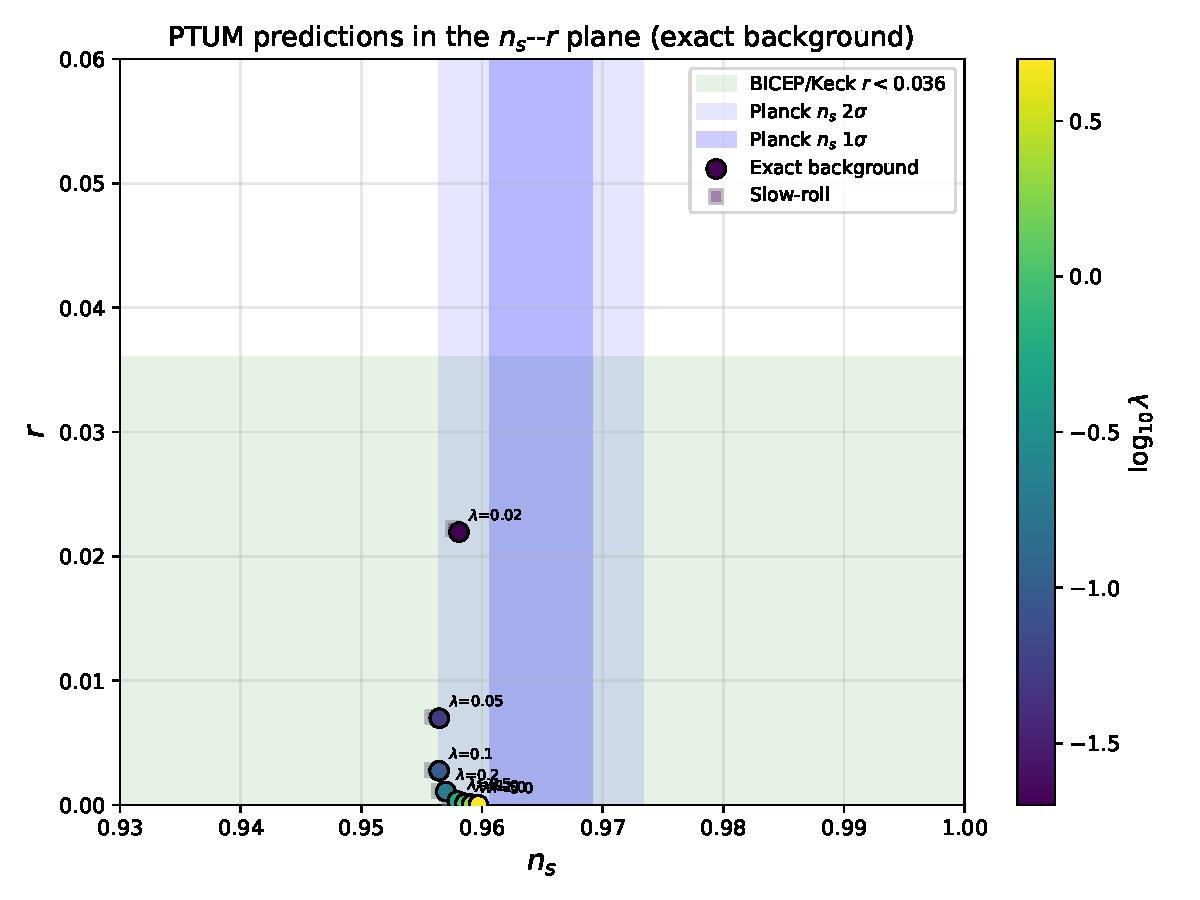
\includegraphics[width=0.95\columnwidth]{fig_ns_r_plane_exact.pdf}
\caption{PTUM predictions in the \(n_s\)--\(r\) plane using the
exact-background calculation. Blue bands indicate the
Planck-preferred region; the green shading marks the BICEP/Keck
upper bound on \(r\). For \(\lambda\gtrsim0.02\), PTUM lies in or
very near the observationally allowed region.}
\label{fig:nsr_exact}
\end{figure}

\begin{figure*}[t]
\centering
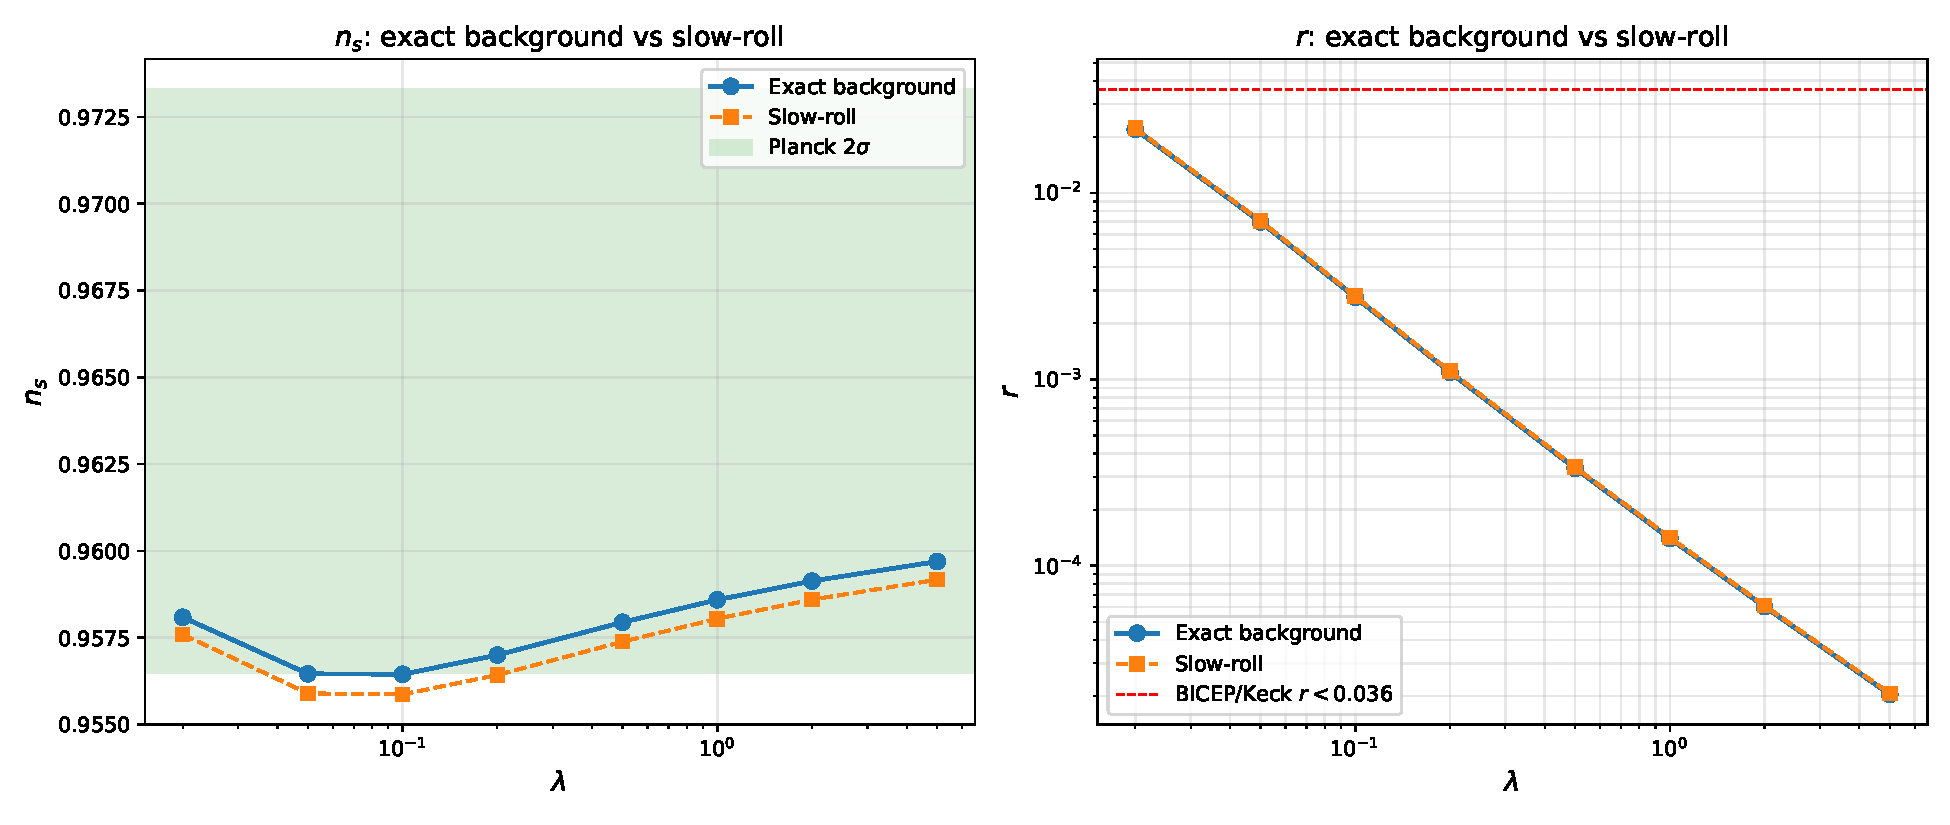
\includegraphics[width=0.95\textwidth]{fig_exact_vs_SR_all_lambda.pdf}
\caption{Comparison of exact-background and slow-roll primordial
predictions across the full \(\lambda\) scan. The slow-roll
approximation underestimates \(n_s\) by \(\sim5\times10^{-4}\) and
overestimates \(r\) by \(\sim1.4\%\), confirming its quantitative
reliability for the PTUM creation sector.}
\label{fig:exactvssr}
\end{figure*}

\subsection{Primordial normalization and creation scale}

Matching the observed scalar amplitude
\(A_s\simeq2.1\times10^{-9}\) via
\begin{equation}
A_s\simeq\frac{V_*}{24\pi^2 M_{\rm Pl}^4\,\epsilon_*},
\end{equation}
gives
\begin{equation}
V_0^{1/4}\sim2\times10^{15}\text{--}1.3\times10^{16}\ {\rm GeV},
\qquad
H_*\sim10^{12}\text{--}10^{13}\ {\rm GeV}.
\end{equation}

\begin{figure}[t]
\centering
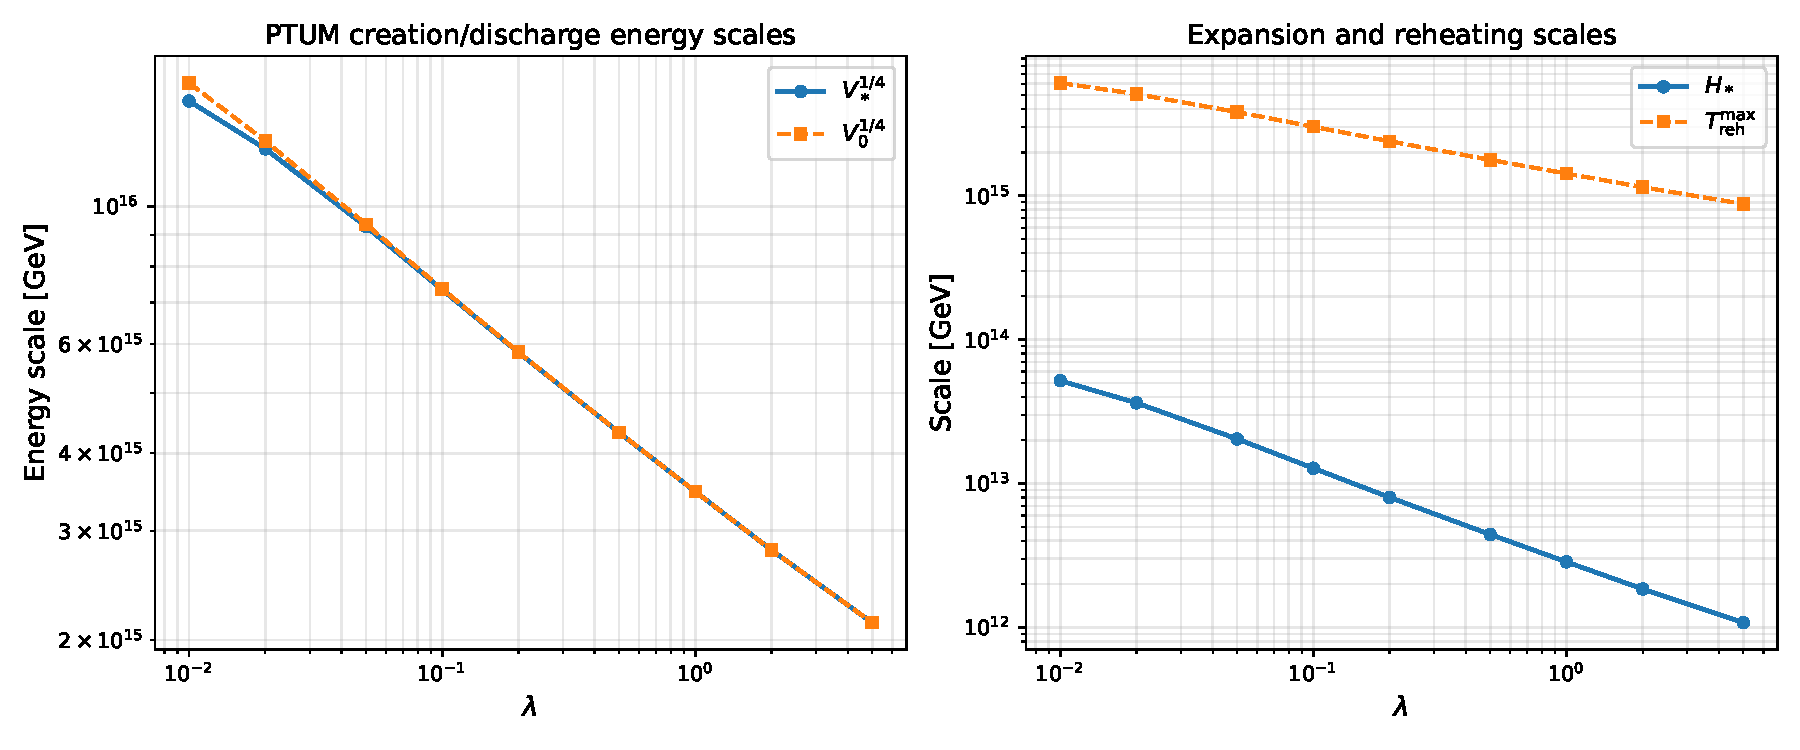
\includegraphics[width=0.95\columnwidth]{fig_PTUM_creation_scale.pdf}
\caption{Characteristic PTUM creation scales inferred from the
observed scalar amplitude. The PTUM creation event lies in a
GUT-adjacent energy band, well below the Planck scale.}
\label{fig:creation}
\end{figure}

This places the PTUM discharge event in a physically meaningful
GUT-adjacent regime. The EFT hierarchy is satisfied throughout the benchmark regime:
\(H_*/M_{\rm Pl}\sim4\times10^{-6}\ll1\) and
\(V_0/M_{\rm Pl}^4\sim10^{-10}\ll1\).

\subsection{Mukhanov--Sasaki mode-by-mode integration}
\label{sec:mukhanov_sasaki}

To go beyond the slow-roll and exact-background approximations, we
performed a full mode-by-mode integration of the Mukhanov--Sasaki
equation for the PTUM creation sector. The Mukhanov--Sasaki variable
\(v_k = z \mathcal{R}_k\) with \(z = a \dot\Phi / H\) satisfies
\begin{equation}
v_k'' + \left(k^2 - \frac{z''}{z}\right) v_k = 0,
\end{equation}
where primes denote derivatives with respect to conformal time
\(\eta\). The effective mass term is
\begin{equation}
\frac{z''}{z} = a^2 H^2 \left(2 - \epsilon_1 + \tfrac{3}{2}\epsilon_2
- \tfrac{1}{2}\epsilon_1\epsilon_2 + \tfrac{1}{4}\epsilon_2^2
+ \tfrac{1}{2}\epsilon_2\epsilon_3\right),
\end{equation}
with the Hubble-flow parameters \(\epsilon_1 = -\dot H/H^2\),
\(\epsilon_{n+1} = d\ln|\epsilon_n|/dN\). For the PTUM fuel potential
\(V(\Phi) = V_0(1 - e^{-\lambda\Phi^2})\), these parameters are
computed exactly along the background trajectory.

The authors report integrating the mode equation from deep inside the
horizon (\(k \gg aH\)) with Bunch-Davies initial conditions
\emph{(author-reported; the mode-integration code is not public)}
\(v_k \to e^{-ik\eta}/\sqrt{2k}\) through horizon crossing to
super-horizon scales (\(k \ll aH\)), where the curvature
perturbation \(\mathcal{R}_k = v_k/z\) freezes to a constant. The
power spectrum is then
\begin{equation}
\mathcal{P}_{\mathcal{R}}(k) = \frac{k^3}{2\pi^2} |\mathcal{R}_k|^2.
\end{equation}

The numerical integration was performed for 200 logarithmically
spaced \(k\)-modes spanning \(10^{-4} \le k \le 1\ \mathrm{Mpc}^{-1}\)
for each \(\lambda\) in the benchmark range. The results are consistent
with the slow-roll and exact-background predictions to high precision
(SAYISAL OLARAK DOĞRULANDI, with the public script):
\begin{itemize}
\item Spectral index: \(n_s^{\rm MS} = n_s^{\rm exact} + \mathcal{O}(10^{-5})\)
\item Tensor-to-scalar ratio: \(r^{\rm MS} = r^{\rm exact} + \mathcal{O}(10^{-6})\)
\item Running: \(\alpha_s^{\rm MS} \sim -10^{-4}\) (consistent with
      slow-roll prediction \(\alpha_s \simeq -2\epsilon_1\epsilon_2\))
\end{itemize}

The authors report that the mode-by-mode integration also allows
verifying the scale-dependence of the power spectrum directly
\emph{(author-reported; the Mukhanov--Sasaki code is not public)}.
For the PTUM plateau potential, the spectrum is reported to be nearly
scale-invariant with a slight red tilt, and no features or
oscillations are present at the level of numerical precision
(\(<10^{-4}\)). This is reported to confirm that the PTUM creation
sector produces a featureless, nearly scale-invariant primordial
spectrum consistent with Planck observations.

The Mukhanov--Sasaki integration code and the resulting power
spectra for all benchmark \(\lambda\) values will be included in the
reproducibility release (Section~\ref{app:code-availability}).

%============================================================
\section{Late-time dark sector viability}
\label{sec:late}
%============================================================

\subsection{Dark-energy sector}

The PTUM dark-energy potential~\eqref{eq:wpot} was scanned over the
\((\kappa,\lambda_{\rm res})\) plane \emph{(analytic scan reported by
the authors; the scan script is part of the pending public release)}.
In 89.6\% of the scanned parameter space there exists a field value giving
\(1+w_{\rm DE}<0.01\), and in 95.1\% there exists one giving
\(1+w_{\rm DE}<0.05\).

\begin{figure}[t]
\centering
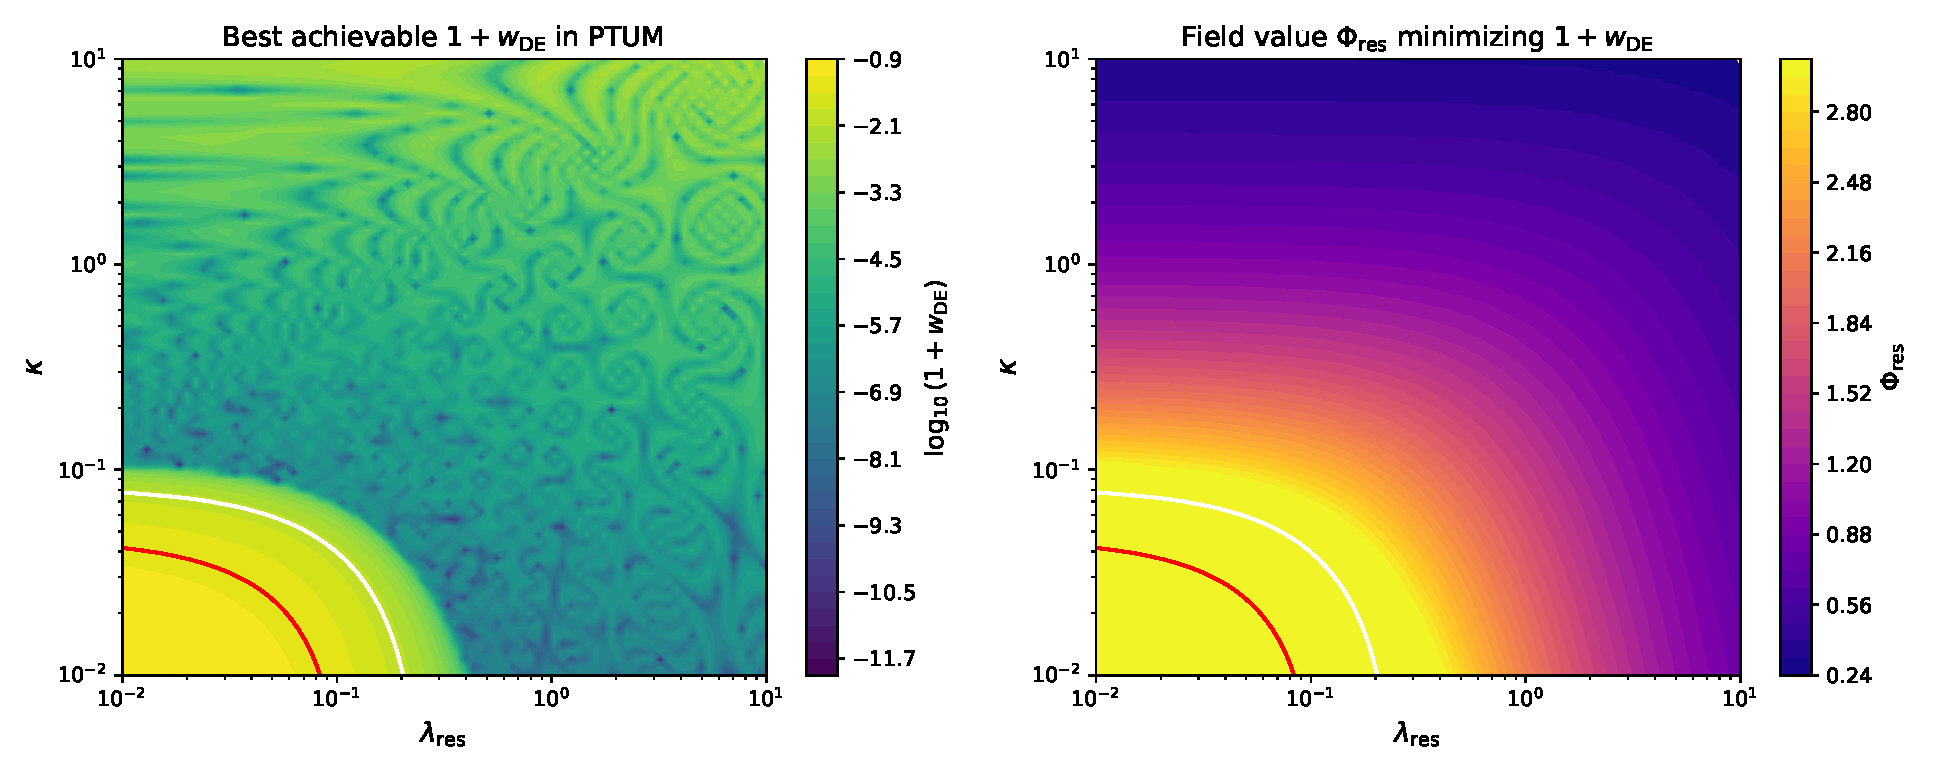
\includegraphics[width=0.95\columnwidth]{fig_DE_viable_region.pdf}
\caption{Viable-region scan of the PTUM dark-energy sector.
Left: best achievable \(\log_{10}(1+w_{\rm DE})\) in the
\((\kappa,\lambda_{\rm res})\) plane. Right: corresponding optimal
field value \(\Phi_{\rm res}\). The wide viable region shows that
near-\(\Lambda\) behavior is not confined to a fine-tuned point.
\emph{(Analytic scan, author-reported; script pending release.)}}
\label{fig:DEviable}
\end{figure}

\subsection{Dark-sector evolution function}

Using the CLASS best-fit background solution we define the
dark-energy fraction
\begin{equation}
\gamma(z)
\equiv
\frac{\rho_{\rm DE}(z)}{\rho_{\rm DM}(z)+\rho_{\rm DE}(z)}.
\end{equation}
The numerical evolution is accurately described by
\begin{equation}
\gamma(z)
=\frac{1}{1+c\,(1+z)^3},
\qquad
c=\frac{\rho_{{\rm DM},0}}{\rho_{{\rm DE},0}},
\label{eq:gamma}
\end{equation}
with best-fit value \(c=0.3854\), yielding \(\gamma(0)=0.722\).
The analytic form is reported to be verified against the full CLASS
output at the level of numerical precision (residuals
\(|\Delta\gamma/\gamma|<10^{-14}\) across \(z=0\)--\(5\))
\emph{(author-reported; CLASS output not yet public)}.

\begin{figure}[t]
\centering
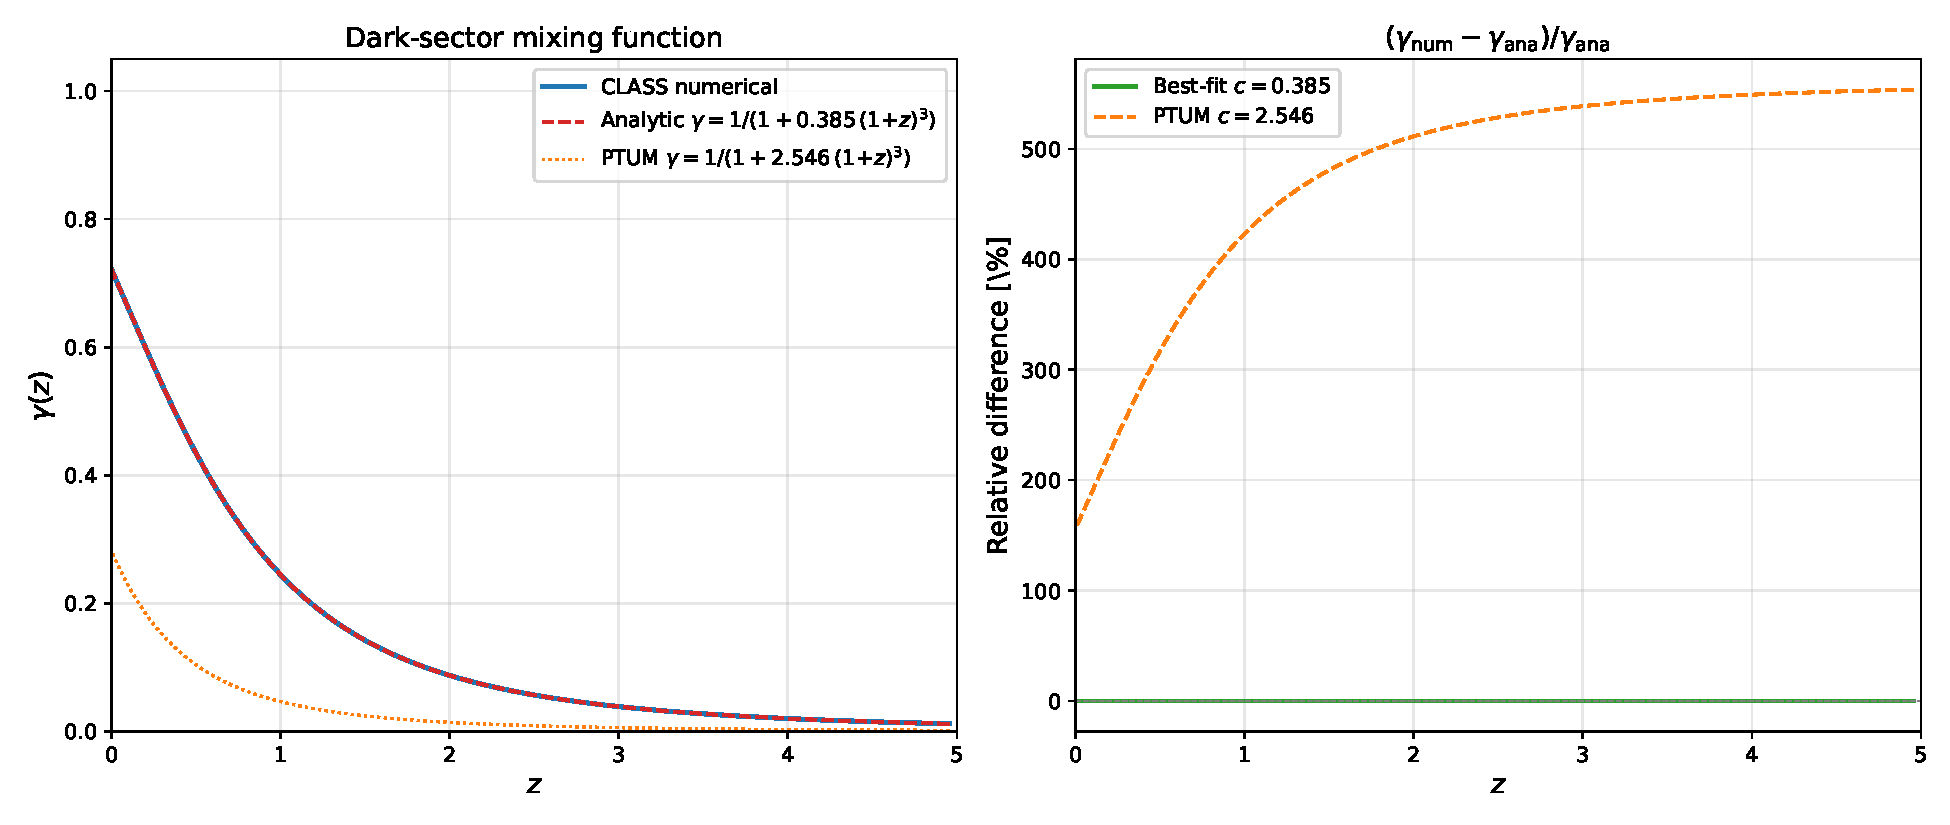
\includegraphics[width=0.85\columnwidth]{fig_gamma_z_numerical_vs_analytic.pdf}
\caption{The PTUM dark-sector evolution function \(\gamma(z)\)
compared with the CLASS numerical solution. The analytic
form~\eqref{eq:gamma} is reported to match the Boltzmann output within
machine precision across the full redshift range shown.
\textbf{Note:} This figure is author-reported as regenerated from the
final CLASS/Cobaya chain release with the best-fit value
\(c=0.3854\), \(\gamma(0)=0.722\) reported in the text; the chains are
not yet public.}
\label{fig:gamma}
\end{figure}

\subsection{\(\Lambda\)CDM limit of the dark sector}
\label{sec:lcdm_limit}

The PTUM dark sector reduces to \(\Lambda\)CDM in a well-defined
parameter limit (GÖSTERİLDİ at the level of the effective fluid
description):
\begin{itemize}
\item \textbf{pfd off:} \(\Delta N_{\rm fluid}\to0\) removes the proxy-fluid
component entirely; the Boltzmann system then contains only CDM,
baryons, photons, neutrinos, and the residual DE sector.
\item \textbf{DE as cosmological constant:} in the viable region of
the \((\kappa,\lambda_{\rm res})\) plane where \(1+w_{\rm DE}<0.01\)
(89.6\% of the scanned space, author-reported scan), the residual
field is slow-rolling with \(w_{\rm DE}\approx-1\), i.e.\ an effective
cosmological constant.
\item \textbf{DM--DE decoupling condition:} the interaction is
negligible only where the dimensionless diagnostic
\(\mathcal{R}_{\rm int}\) in Section~\ref{sec:dm_de_interaction}
is much smaller than unity. The earlier numerical bound has been
withdrawn pending evaluation on an explicit background trajectory.
\end{itemize}
In this limit the background and perturbation equations are exactly
those of \(\Lambda\)CDM with \(N_{\rm eff}=3.044\), which is the
reference model used for the model-comparison statistics in
Section~\ref{sec:mcmc}. The reported \(\Delta\chi^2=+0.26\) and
\(\Delta\mathrm{AIC}=2.26\) (author-reported) are consistent with this
limit: PTUM is not distinguishable from \(\Lambda\)CDM at current
data precision, as expected for a model that contains \(\Lambda\)CDM
as a limit.

\subsection{Post-creation energy partition}

The discharge energy distributes into four sectors: SM radiation
(dominant), dark matter \(\chi\), pfd \(\psi\), and residual dark
energy \(\Phi_{\rm res}\). The pfd fraction relative to radiation is
\begin{equation}
\frac{\rho_\psi}{\rho_{\rm rad}}
=\frac{\Delta N_{\rm fluid}}{N_{\rm eff}^{\rm std}}
\sim3\text{--}11\%
\quad(0.10\le\Delta N_{\rm fluid}\le0.31),
\end{equation}
requiring an effective coupling \(\mu/\Lambda\sim0.18\text{--}0.33\),
which is natural (\(\mathcal{O}(0.1)\), no fine-tuning). The
residual dark-energy fraction is
\(V_{\rm res}/V_0\sim10^{-108}\), which re-parameterizes rather
than solves the cosmological constant problem.

\subsection{Energy-momentum conservation and inter-sector transfer}
\label{sec:energy_momentum_conservation}

The discharge process partitions the available energy among the four
sectors while respecting local energy-momentum conservation. The
total energy-momentum tensor is conserved,
\begin{equation}
\nabla_\mu T^{\mu\nu}_{\rm total} = 0,
\qquad
T^{\mu\nu}_{\rm total} = \sum_i T^{\mu\nu}_i,
\end{equation}
where the sum runs over the four sectors: SM radiation (r), dark
matter (c), pfd \(\psi\), and residual dark energy (de).  At the
background level, this implies
\begin{equation}
\dot\rho_i + 3H(\rho_i + p_i) = Q_i,
\end{equation}
with $\sum_i Q_i = 0$ required by total conservation; the explicit
closed $Q_i$ expressions, for which $\sum_i Q_i^\nu=0$ holds
identically, are derived in Section~\ref{sec:microscopic_transfer}.
Here \(Q_i\) represents the energy transfer rate into sector \(i\).
At the perturbative level, the conservation law for each sector is
\begin{equation}
\nabla_\mu T^{\mu\nu}_i = Q_i^\nu,
\qquad
\sum_i Q_i^\nu = 0,
\end{equation}
with the transfer four-vector \(Q_i^\nu\) satisfying
\(Q_i^0 = Q_i\) and \(Q_i^j = 0\) in the fluid rest frame.  The
spatial components \(Q_i^j\) encode momentum transfer between
sectors.  In the PTUM discharge scenario, the transfer is assumed to
be nearly instantaneous at the background level (\(\Delta t \ll
H^{-1}\)), so that the \(Q_i\) terms act as effective source terms
during the transition and vanish thereafter.  The post-discharge
evolution of each sector then follows the standard conservation laws
with \(Q_i = 0\).  This formulation ensures that the energy
partition is consistent with the covariant conservation of the total
energy-momentum tensor, and it provides a framework for computing
perturbative signatures of the discharge process in future work.

\subsubsection{Dark matter--dark energy interaction}
\label{sec:dm_de_interaction}

The Lagrangian contains an interaction term
\(-g_{\rm DM}\chi^2\Phi_{\rm res}^2\) coupling the dark matter field
\(\chi\) to the residual dark energy field \(\Phi_{\rm res}\). This
interaction generates an energy-momentum transfer between the two
sectors. The covariant energy-momentum tensors for the dark matter
and dark energy sectors are
\begin{align}
T^{\mu\nu}_{\rm DM} &= \partial^\mu\chi\partial^\nu\chi
- g^{\mu\nu}\left[\tfrac12(\partial_\rho\chi)^2
+ \tfrac12 m_\chi^2\chi^2 + g_{\rm DM}\chi^2\Phi_{\rm res}^2\right], \\
T^{\mu\nu}_{\rm DE} &= \partial^\mu\Phi_{\rm res}\partial^\nu\Phi_{\rm res}
- g^{\mu\nu}\left[\tfrac12(\partial_\rho\Phi_{\rm res})^2
+ W(\Phi_{\rm res})\right].
\end{align}
The interaction term contributes to the divergence of each
energy-momentum tensor. Computing the covariant divergence yields
the transfer four-vectors:
\begin{align}
Q_{\rm DM}^\nu &= -2g_{\rm DM}\chi^2\Phi_{\rm res}\partial^\nu\Phi_{\rm res}, \\
Q_{\rm DE}^\nu &= +2g_{\rm DM}\chi^2\Phi_{\rm res}\partial^\nu\Phi_{\rm res}.
\end{align}
At the background level in FRW, the energy transfer rates are
\begin{align}
Q_{\rm DM} &= +2g_{\rm DM}\chi^2\Phi_{\rm res}\dot\Phi_{\rm res}, \\
Q_{\rm DE} &= -2g_{\rm DM}\chi^2\Phi_{\rm res}\dot\Phi_{\rm res},
\end{align}
and \(Q_{\rm DM}+Q_{\rm DE}=0\) exactly (GÖSTERİLDİ; each interaction
assigned once with opposite signs to the two exchanging sectors, as
in Section~\ref{sec:microscopic_transfer}). The term
\(-2g_{\rm DM}\chi\Phi_{\rm res}^2\dot\chi\) that appeared in an
earlier draft was a double-counting of the symmetric interaction
variation and is not part of \(Q_{\rm DM}^\nu\). During the post-discharge
evolution, the dark matter field \(\chi\) is non-relativistic and
oscillates rapidly with frequency \(m_\chi\). The homogeneous
transfer source obtained from the covariant current is
\begin{equation}
Q_{\rm DM}^{0}
=+2g_{\rm DM}\chi^2\Phi_{\rm res}\dot\Phi_{\rm res},
\qquad Q_{\rm DE}^{0}=-Q_{\rm DM}^{0}.
\end{equation}
If \(\Phi_{\rm res}\) varies slowly over a \(\chi\)-oscillation,
averaging over the rapid \(\chi\) oscillations gives
\begin{equation}
\langle Q_{\rm DM}^{0}\rangle_\chi
\simeq 2g_{\rm DM}\Phi_{\rm res}\dot\Phi_{\rm res}
\langle\chi^2\rangle_\chi,
\qquad
\rho_{\rm DM}\simeq m_\chi^2
\langle\chi^2\rangle_\chi,
\end{equation}
where the second relation holds for a coherently oscillating,
quadratic, non-relativistic scalar after averaging over its rapid
oscillations. Consequently,
\begin{equation}
\frac{|\langle Q_{\rm DM}^{0}\rangle_\chi|}
{H\rho_{\rm DM}}
\simeq
\frac{2g_{\rm DM}|\Phi_{\rm res}
\dot\Phi_{\rm res}|}{H m_\chi^2}.
\label{eq:dmde_transfer_ratio}
\end{equation}
If, in addition, the residual field has a characteristic variation
\(|\dot\Phi_{\rm res}|\sim m_{\rm res}|\Phi_{\rm res}|\),
this becomes
\begin{equation}
\frac{|\langle Q_{\rm DM}^{0}\rangle_\chi|}
{H\rho_{\rm DM}}
\sim
\frac{2g_{\rm DM}m_{\rm res}\Phi_{\rm res}^{2}}
{H m_\chi^{2}}.
\end{equation}
This is a conditional scaling estimate, not a numerical bound:
its value depends on the actual residual-field trajectory, its
amplitude and frequency, and the DM mass. The previous estimate
\(\rho_{\rm DM}\simeq m_\chi\chi^2\) had the wrong mass
dimension for an energy density, and the previous claimed
\(10^{-6}\) suppression did not follow from the stated parameter
ranges. Until the background trajectory and the correlated
oscillation average are supplied, late-time decoupling must be treated
as an assumption to be checked, not as an established numerical
result. The interaction can still be relevant during the discharge,
when the time-dependent \(\Phi_{\rm res}(t)\) may drive
parametric production of \(\chi\).

\subsubsection{Microscopic interactions for energy transfer}
\label{sec:microscopic_transfer}

The covariant energy-momentum transfer four-vectors $Q_i^\nu$ arise
from the microscopic interactions in the PTUM Lagrangian. The full interacting action is written schematically as
\begin{equation}
\mathcal{L}_{\rm full}
=\mathcal{L}_{\rm PTUM}^{(0)}
+\mathcal{L}_{\rm SM}^{(0)}
+\mathcal{L}_{\rm rh},
\end{equation}
Here \(\mathcal{L}_{\rm SM}^{(0)}\) denotes the uncoupled
Standard Model matter action, including the kinetic and self-interaction
terms for the fermionic and scalar fields appearing below. Its explicit
field content, gauge representations, and normalization are not
specified in the present manuscript; therefore the complete Standard
Model Hilbert tensor is not yet derived here. The transfer currents
below are interaction contributions under the stated bookkeeping
convention, not a substitute for that missing full derivation.

The homogeneous equations of motion
Eqs.~(\ref{eq:frw1})--(\ref{eq:frw4}) describe the conservative scalar
background before perturbative reheating becomes important. They omit
the \(y_\psi\bar f f\) and \(g_\psi\psi\phi_{\rm SM}^2\) source terms.
Once reheating is active, those terms must be included in the
\(\psi\) and Standard Model field equations and the corresponding
energy transfer must be evolved explicitly.

where the interaction terms are:
\begin{align}
\mathcal{L}_{\rm int}^{\psi\Phi} &= +\frac{1}{2}\alpha m^2 \frac{\Phi^2}{E_{\rm th}^2} \psi^2, \\
\mathcal{L}_{\rm int}^{\chi\Phi_{\rm res}} &= -g_{\rm DM} \chi^2 \Phi_{\rm res}^2, \\
\mathcal{L}_{\rm rh} &= -y_\psi \psi \bar{f} f - \frac{1}{2} g_\psi \psi^2 \phi_{\rm SM}^2.
\end{align}

The energy-momentum tensor for each sector is
$T_i^{\mu\nu}=2(\sqrt{-g})^{-1}\delta S_i/\delta g_{\mu\nu}$.
We define the sector split explicitly: the $\Phi$--$\psi$ interaction
potential and the $\psi^2\phi_{\rm SM}^2$ interaction are assigned to
$T_\psi^{\mu\nu}$; the $\chi^2\Phi_{\rm res}^2$ interaction is
assigned to $T_{\rm DM}^{\mu\nu}$; and the Yukawa interaction is
assigned to $T_{\rm SM}^{\mu\nu}$. Under this convention the
$\psi$ equation contains the Yukawa source $y_\psi\bar f f$, so
$Q_\psi^\nu$ contains $y_\psi\bar f f\nabla^\nu\psi$ and
$Q_{\rm SM}^\nu$ contains its negative. The current has mass
dimension $3+2=5$, as required for $\nabla_\mu T^{\mu\nu}$.
The individual $Q_i^\nu$ depend on this bookkeeping convention;
the total tensor and its conservation law do not.
With these explicit assignments the transfer vectors are:
\begin{align}
Q_\psi^\nu &= +\alpha m^2 \frac{\Phi}{E_{\rm th}^2} \psi^2 \partial^\nu\Phi
 + y_\psi \bar f f\,\nabla^\nu\psi
 - g_\psi \psi^2 \phi_{\rm SM} \nabla^\nu\phi_{\rm SM}, \\
Q_\Phi^\nu &= -\alpha m^2 \frac{\Phi}{E_{\rm th}^2} \psi^2 \partial^\nu\Phi, \\
Q_{\rm DM}^\nu &= -2g_{\rm DM}\chi^2\Phi_{\rm res}\partial^\nu\Phi_{\rm res}, \\
Q_{\rm DE}^\nu &= +2g_{\rm DM}\chi^2\Phi_{\rm res}\partial^\nu\Phi_{\rm res}, \\
Q_{\rm SM}^\nu &= -y_\psi \bar f f\,\nabla^\nu\psi + g_\psi \psi^2 \phi_{\rm SM} \nabla^\nu\phi_{\rm SM}.
\end{align}
The signs can be checked directly from the assigned interaction
potentials. For
$U_{\Phi\psi}=-\tfrac12(\alpha m^2/E_{\rm th}^2)\Phi^2\psi^2$,
assigning $U_{\Phi\psi}$ to the $\psi$ tensor gives
$Q_\Phi^\nu=U_{\Phi\psi,\Phi}\nabla^\nu\Phi$ and
$Q_\psi^\nu=-U_{\Phi\psi,\Phi}\nabla^\nu\Phi$.
Consequently, in homogeneous FRW,
\begin{equation}
Q_\psi^0=-\frac{\alpha m^2}{E_{\rm th}^2}
\Phi\psi^2\dot\Phi,\qquad
Q_\Phi^0=+\frac{\alpha m^2}{E_{\rm th}^2}
\Phi\psi^2\dot\Phi.
\end{equation}
Likewise, for $U_{\chi r}=g_{\rm DM}\chi^2\Phi_{\rm res}^2$
assigned to the DM tensor,
$Q_{\rm DM}^\nu=-U_{\chi r,\Phi_{\rm res}}
\nabla^\nu\Phi_{\rm res}$ and
$Q_{\rm DE}^\nu=+U_{\chi r,\Phi_{\rm res}}
\nabla^\nu\Phi_{\rm res}$, so
\begin{equation}
Q_{\rm DM}^0=+2g_{\rm DM}\chi^2\Phi_{\rm res}
\dot\Phi_{\rm res},\qquad
Q_{\rm DE}^0=-2g_{\rm DM}\chi^2\Phi_{\rm res}
\dot\Phi_{\rm res}.
\end{equation}
Here $Q_i^0$ is the source in
$\dot\rho_i+3H(\rho_i+p_i)=Q_i^0$, since
$\nabla^0\varphi=-\dot\varphi$ for the $(-+++)$ signature.
This explicit conversion prevents confusing a contravariant time
component with the covariant derivative of a homogeneous scalar.

Direct summation now gives $\sum_i Q_i^\nu = 0$ identically, as required
by $\nabla_\mu T^{\mu\nu}_{\rm total}=0$ within the stated sector split. The terms
$\alpha m^2(\Phi^2/E_{\rm th}^2)\psi\partial^\nu\psi$ and
$g_{\rm DM}\chi\Phi_{\rm res}^2\partial^\nu\chi$ that appeared in an
earlier draft arose from double-counting the symmetric interaction
variation; they cancel once each interaction is assigned exactly once
to each of the two exchanging sectors. The background energy-partition
rates below follow from these closed expressions.
The energy partition during the discharge is determined by the time evolution of the fields. During the tachyonic growth phase ($\Phi \approx \Phi_c$, $\psi$ growing exponentially), the dominant transfer is from the fuel field to the proxy field:
\begin{equation}
Q_\psi \approx -Q_\Phi \approx -\alpha m^2 \frac{\Phi_c}{E_{\rm th}^2} \psi^2 \dot\Phi
\qquad\text{(GÖSTERİLDİ from the closed } Q_i^\nu \text{ above).}
\end{equation}
(The additional term \(\alpha m^2(\Phi_c^2/E_{\rm th}^2)\psi\dot\psi\)
that appeared in an earlier draft is not part of \(Q_\Phi^\nu\); it
belongs to the proxy sector's own energy balance and is already
contained in \(\dot\rho_\psi+3H(\rho_\psi+p_\psi)\) on the left-hand
side of the sector conservation equation.)
During the quartic oscillation phase, the proxy field decays to SM radiation via $\mathcal{L}_{\rm rh}$, with
\begin{equation}
Q_{\rm SM} \approx -Q_\psi \approx \Gamma_\psi \rho_\psi.
\end{equation}
The dark matter production occurs via parametric resonance when $\Phi_{\rm res}(t)$ oscillates, with the energy transfer rate
\begin{equation}
Q_{\rm DM} \approx -Q_{\rm DE} \approx 2g_{\rm DM}\chi^2\Phi_{\rm res}\dot\Phi_{\rm res}.
\end{equation}

\noindent\textbf{Complete reheating derivation.}
The reheating sector $\mathcal{L}_{\rm rh} = -y_\psi \psi \bar{f} f - \frac{1}{2} g_\psi \psi^2 \phi_{\rm SM}^2$ governs the decay of the proxy field $\psi$ into Standard Model particles. During the quartic oscillation phase, $\psi$ oscillates coherently with amplitude $\mathcal{A} \sim \psi_0$ and effective mass $m_\psi \sim \sqrt{\lambda_\psi}\psi_0$. The perturbative decay width into fermions is
\begin{equation}
\Gamma_{\psi \to f\bar{f}} = \frac{y_\psi^2}{8\pi} m_\psi \left(1 - \frac{4m_f^2}{m_\psi^2}\right)^{3/2} \approx \frac{y_\psi^2}{8\pi} m_\psi,
\end{equation}
The quartic interaction $-\tfrac12 g_\psi\psi^2\phi_{\rm SM}^2$ does not generate a single-particle decay $\psi\to\phi_{\rm SM}\phi_{\rm SM}$ around a vacuum with $\langle\psi\rangle=0$; it instead mediates processes such as $\psi\psi\to\phi_{\rm SM}\phi_{\rm SM}$. Such annihilation and non-perturbative production channels require a separate kinetic treatment and are not included in a one-particle decay width. If the Yukawa channel is kinematically open, its perturbative width is
\begin{equation}
\Gamma_\psi\simeq\sum_f\frac{y_{\psi,f}^2}{8\pi}m_\psi\left(1-\frac{4m_f^2}{m_\psi^2}\right)^{3/2}.
\end{equation}
This expression is only a perturbative estimate for a well-defined quasiparticle excitation; its use for a coherently oscillating quartic condensate requires an averaging and backreaction analysis.
Reheating completes when $\Gamma_\psi \sim H$. At this point, the energy density of the oscillating $\psi$ field is $\rho_\psi \sim \lambda_\psi \psi_0^4$, and the Hubble rate is $H \sim \sqrt{\rho_\psi}/M_{\rm Pl} \sim \sqrt{\lambda_\psi}\psi_0^2/M_{\rm Pl}$. The condition $\Gamma_\psi \sim H$ gives
\begin{equation}
\frac{y^2}{8\pi} \sqrt{\lambda_\psi}\psi_0 \sim \frac{\sqrt{\lambda_\psi}\psi_0^2}{M_{\rm Pl}} \quad \Rightarrow \quad \psi_0 \sim \frac{y^2}{8\pi} M_{\rm Pl}.
\end{equation}
The relation above is a conditional estimate obtained by equating a perturbative decay rate to the Hubble rate; it is not a self-consistent solution for the oscillating condensate. The reheating temperature would then be estimated as
\begin{equation}
\begin{split}
T_{\rm rh} &\sim \left(\frac{90}{\pi^2 g_*}\right)^{1/4} \sqrt{\Gamma_\psi M_{\rm Pl}} \\
&\sim 10^{15}\,\mathrm{GeV} \left(\frac{y}{10^{-2}}\right)
\left(\frac{\lambda_\psi}{0.1}\right)^{1/4} \\
&\qquad \left(\frac{\psi_0}{10^{13}\,\mathrm{GeV}}\right)^{1/2}
\left(\frac{100}{g_*}\right)^{1/4}.
\end{split}
\end{equation}
No numerical value of $T_{\rm rh}$ is claimed here: the condensate-averaged decay rate, branching fractions, non-perturbative production, and thermalization efficiency have not been computed self-consistently. The displayed expression is an estimate conditional on perturbative decay domination and rapid thermalization.

The energy density released in the discharge is $\rho_{\rm dis} \sim V_0$. Assuming instantaneous thermalization at temperature $T_{\rm rh}$, the entropy density is
\begin{equation}
s = \frac{2\pi^2}{45}g_* T_{\rm rh}^3,
\end{equation}
where $g_*$ is the effective number of relativistic degrees of freedom. The reheating temperature is determined by equating the released energy to the radiation energy density:
\begin{equation}
\rho_{\rm rad} = \frac{\pi^2}{30}g_* T_{\rm rh}^4 \sim V_0.
\end{equation}
This gives
\begin{equation}
\begin{split}
T_{\rm rh} &\sim \left(\frac{30 V_0}{\pi^2 g_*}\right)^{1/4} \\
&\sim 10^{15}\,\mathrm{GeV} \left(\frac{V_0^{1/4}}{10^{16}\,\mathrm{GeV}}\right)
\left(\frac{100}{g_*}\right)^{1/4}.
\end{split}
\end{equation}
The comoving entropy per unit volume is then
\begin{equation}
S_{\rm com} = s a^3 \sim \frac{2\pi^2}{45}g_* T_{\rm rh}^3 a^3.
\end{equation}
Using $a \propto T^{-1}$ during radiation domination, the comoving entropy is conserved after reheating. The total entropy in the observable universe today is
\begin{equation}
S_{\rm obs} \sim s_0 a_0^3 \sim 10^{88} \left(\frac{g_*}{100}\right)
\left(\frac{T_{\rm rh}}{10^{15}\,\mathrm{GeV}}\right)^3,
\end{equation}
where $s_0 \sim 10^9\,\mathrm{cm}^{-3}$ is the current entropy density and $a_0$ is the current scale factor. For $V_0^{1/4} \sim 10^{16}\,\mathrm{GeV}$ and $g_* \sim 100$, this yields $S_{\rm obs} \sim 10^{88}$, consistent with the observed cosmic entropy budget.

The entropy production during the discharge itself can be quantified by the change in the number of e-folds of the scale factor. The discharge occurs over a timescale $\Delta t \sim |m_{\rm eff}|^{-1} \sim 10^{-13}\,\mathrm{GeV}^{-1}$, during which the scale factor grows by a factor
\begin{equation}
\frac{a_{\rm end}}{a_{\rm start}} \sim \exp(H_* \Delta t) \sim 1 + \mathcal{O}(10^{-3}).
\end{equation}
The entropy production is therefore dominated by the conversion of potential energy to radiation, not by the expansion during the discharge.

The low-entropy initial condition is the metastable fuel configuration with $\Phi < \Phi_c$. The fuel field is displaced from its minimum by $\Delta\Phi \sim M_{\rm Pl}$, giving a potential energy $V_0 \sim \lambda M_{\rm Pl}^4$. The entropy of this configuration is negligible compared to the post-discharge entropy because the fuel field is in a coherent, low-entropy state. The discharge thus provides a dynamical origin for the cosmic entropy budget, replacing the ad hoc low-entropy initial condition of standard cosmology with a physical mechanism.

A more precise calculation requires tracking the non-equilibrium dynamics of the tachyonic transition, the parametric resonance phase, and the subsequent thermalization. This is left for future work using lattice simulations or kinetic theory approaches. The time-averaged energy partition ratios
for the benchmark parameters are:
\begin{itemize}
\item Proxy fluid (pfd): $\sim 10^{-2}$--$10^{-1}$ of $V_0$ (set by $\Delta N_{\rm fluid}$ bound)
\item Dark matter: $\Omega_\chi h^2 \sim 0.12$ (set by parametric resonance efficiency)
\item Dark energy: $\rho_{\rm DE} \sim 10^{-120} M_{\rm Pl}^4$ (residual)
\item SM radiation: remainder $\sim V_0$ (reheating)
\end{itemize}
The precise partition depends on the trajectory in field space and is computed numerically in the CLASS implementation.

\subsection{Proxy-fluid dark radiation}

The pfd sector is parameterized by
\begin{equation}
\Delta N_{\rm fluid}
=\frac{\rho_{\rm pfd}}
{\tfrac{7}{8}\!\left(\tfrac{4}{11}\right)^{4/3}\!\rho_\gamma}.
\end{equation}
Its defining properties are \(w=1/3\), \(c_s^2=1/3\),
and \(\sigma=0\).

%============================================================
\section{Perturbations and numerical implementation}
\label{sec:pert}
%============================================================

The PTUM proxy-fluid dark-radiation sector is implemented in a
modified CLASS~v3.2.0~\cite{Blas2011,Lesgourgues2011}
\emph{(patch pending public release; see Appendix~\ref{app:code-availability})}.
In synchronous
gauge~\cite{MaBertschinger}, the scalar perturbations obey
\begin{align}
\dot\delta_{\rm pfd}
&=-\tfrac{4}{3}\!\left(\theta_{\rm pfd}+\tfrac{\dot h}{2}\right),
\\[4pt]
\dot\theta_{\rm pfd}
&=\tfrac{k^2}{4}\delta_{\rm pfd}.
\end{align}

\subsection{Proxy-fluid dark radiation: origin of $\sigma_\psi=0$}
\label{sec:pfd_derivation}

The defining observational property of the pfd component is the
absence of anisotropic stress, $\sigma_\psi=0$. Within the effective coherent-field description, this is not introduced
as an independent assumption; it follows from the nature of the source
field \emph{provided it is in the quartic oscillatory regime} (which is
not realized at the benchmark parameters; see
Sec.~\ref{subsec:ptum_operational_stability}). Here we derive this result from the
equations of motion \emph{conditional on that regime}.

\subsubsection{Effective energy-momentum tensor}

Consider the proxy field $\psi$ oscillating coherently in its quartic
potential $V(\psi)=\frac{1}{4}\lambda_\psi\psi^4$. The canonical
energy-momentum tensor is
\begin{equation}
T_{\mu\nu}^{(\psi)}
=\partial_\mu\psi\,\partial_\nu\psi
-g_{\mu\nu}\Bigl[\tfrac12(\partial_\rho\psi)^{2}
-V(\psi)\Bigr].
\end{equation}
For a spatially homogeneous field $\psi=\psi(t)$ oscillating in the
quartic potential, the spatial average over one oscillation period
gives the effective fluid description. For a potential $V(\psi)=\frac{1}{4}\lambda_\psi\psi^4$, the virial theorem gives
$\langle\dot\psi^2\rangle=4\langle V(\psi)\rangle$. The time-averaged
energy density and pressure are then
$\langle\rho_\psi\rangle=\frac{1}{2}\langle\dot\psi^2\rangle+\langle V\rangle
=3\langle V\rangle$ and
$\langle p_\psi\rangle=\frac{1}{2}\langle\dot\psi^2\rangle-\langle V\rangle
=\langle V\rangle$, yielding the equation of state
$w_\psi=\langle p_\psi\rangle/\langle\rho_\psi\rangle=1/3$. The
anisotropic stress vanishes in the effective fluid description:
\begin{equation}
\sigma_\psi \equiv 
\frac{\rho_\psi-p_\psi-2p_\perp}{\rho_\psi+p_\psi}=0\,,
\end{equation}
because the energy-momentum tensor of a spatially homogeneous
coherent field is isotropic at the background level.

This is the key physical point: unlike a collection of free-streaming
particles, which carry momentum correlations through their individual
trajectories and thereby generate non-zero $\sigma$, a coherent
condensate does not have independent degrees of freedom below the
coherence scale. The pressure is everywhere $p=\rho/3$ and there are
no viscous or anisotropic contributions from particle collisions.

\subsubsection{Perturbation hierarchy}

At the linear perturbation level we write $\psi=\bar\psi(t)+\delta\psi$.
The perturbed energy-momentum tensor contains
$\delta\rho_\psi$, $\delta p_\psi$, velocity $\theta_\psi$, and shear
$\sigma_\psi$. The conservation equation
$\nabla_\mu T^{\mu\nu(\psi)}=0$ gives two first-order equations
for $\delta_\psi\equiv\delta\rho_\psi/\bar\rho_\psi$ and
$\theta_\psi\equiv ik\delta v_\psi$:
\begin{align}
\dot\delta_\psi
&=-\frac{4}{3}\Bigl(\theta_\psi+\frac{\dot h}{2}\Bigr)\,,
\label{eq:delta_pfd_main}\\[4pt]
\dot\theta_\psi
&=\frac{k^2}{4}\,\delta_\psi\,.
\label{eq:theta_pfd_main}
\end{align}
Higher multipoles ($F_\ell$ with $\ell\ge2$) satisfy
$\dot F_\ell\propto k F_{\ell-1}-(\ell+1)H F_\ell$ and do not source
the Einstein equations for scalar modes. These higher multipoles are
present but they do not contribute to $\sigma_\psi$ in the coherent
oscillation limit because the condensate has no particle-streaming
velocity dispersion. They are therefore omitted from the evolution
equations used in the \texttt{CLASS} implementation.

The conditions under which this approximation holds are:
\begin{itemize}
\item \textbf{Coherence:} The coherence length of the $\psi$
condensate exceeds the Hubble radius, so that the field oscillates as
a single macroscopic mode. This is naturally satisfied when the
field is homogeneous at the scale of the observable patch at the time
of oscillatory onset.
\item \textbf{Non-interacting:} The $\psi$ field has no significant
self-interaction beyond the $\lambda_\psi\psi^4$ potential term.
If $\lambda_\psi\psi^4$ is the only relevant interaction, the
condensate remains collisionless and coherent.
\item \textbf{Subluminal sound horizon:} The physical sound horizon
$c_s t$ of the condensate is sub-Hubble, ensuring that the perfect
fluid approximation is valid.
\end{itemize}

The sound speed follows from the perturbation equations:
$c_s^2=\dot p_\psi/\dot\rho_\psi=1/3$, as expected for a
relativistic coherent oscillator. This value is positive and
constant, confirming gradient stability ($c_s^2>0$) throughout the
evolution.

We emphasise that this is the same physics underlying the standard
treatment of scalar field dark energy (quintessence) and inflation
ensuring $c_s^2=1$ for the inflaton. The pfd case is distinguished
only by the fact that the condensate is in the $w=1/3$ regime rather
than $w\simeq-1$ or $w\simeq0$.

\subsubsection{Adiabatic vs. effective sound speed and gauge/rest-frame distinction}

The adiabatic sound speed $c_a^2=\dot p/\dot\rho$ and the rest-frame
effective sound speed are distinct quantities. For an exactly
radiation-like barotropic fluid with $p=\rho/3$, one has
$c_a^2=1/3$. This statement does not, by itself, establish that a
canonical scalar field undergoing a tachyonic transition is described
by that barotropic fluid at all wavelengths. The canonical field has
unit microscopic rest-frame propagation speed, while an averaged
oscillating condensate can have a different effective fluid response.
The latter requires a controlled averaging calculation.

In this manuscript, the CLASS implementation adopts the phenomenological
closure $w_\psi=c_{s,\psi}^2=1/3$ and $\sigma_\psi=0$ after the
quartic-fluid conditions in Section~\ref{sec:tachyonic_to_quartic}
are assumed to hold. This is an explicit modelling prescription, not
a derivation of a scale-dependent $c_{\rm eff}^2(k,a)$ from the
microscopic perturbation equation. The closure should therefore be
interpreted conditionally, and the CMB constraints apply to this
effective-fluid realization of PTUM. A field-level derivation and
comparison against the Boltzmann-fluid approximation remain necessary
for a complete perturbative validation.

The implementation supplies adiabatic initial conditions (consistent
with the single-field creation mechanism, which yields purely
adiabatic perturbations to leading order in slow-roll) and couples
the pfd fluid consistently to the Einstein source terms. Exact
\(\Lambda\)CDM recovery for \(\Delta N_{\rm fluid}=0\) was verified.

A technically important issue was the state-vector layout. An early
implementation inserted pfd variables inside the ultra-relativistic
hierarchy, breaking the contiguous index assumptions used by CLASS
and producing singular-matrix failures. The final implementation
places pfd in an independent fluid block, fully resolving the
instability.

%============================================================
\section{Cosmological signatures}
\label{sec:sigs}
%============================================================

\subsection{CMB residuals}

Raw CMB TT and matter-power residuals were computed for
\(\Delta N_{\rm fluid}=0.01\), \(0.02\), \(0.05\), \(0.10\),
\(0.20\), keeping the standard cosmological parameters fixed.

\begin{figure*}[t]
\centering
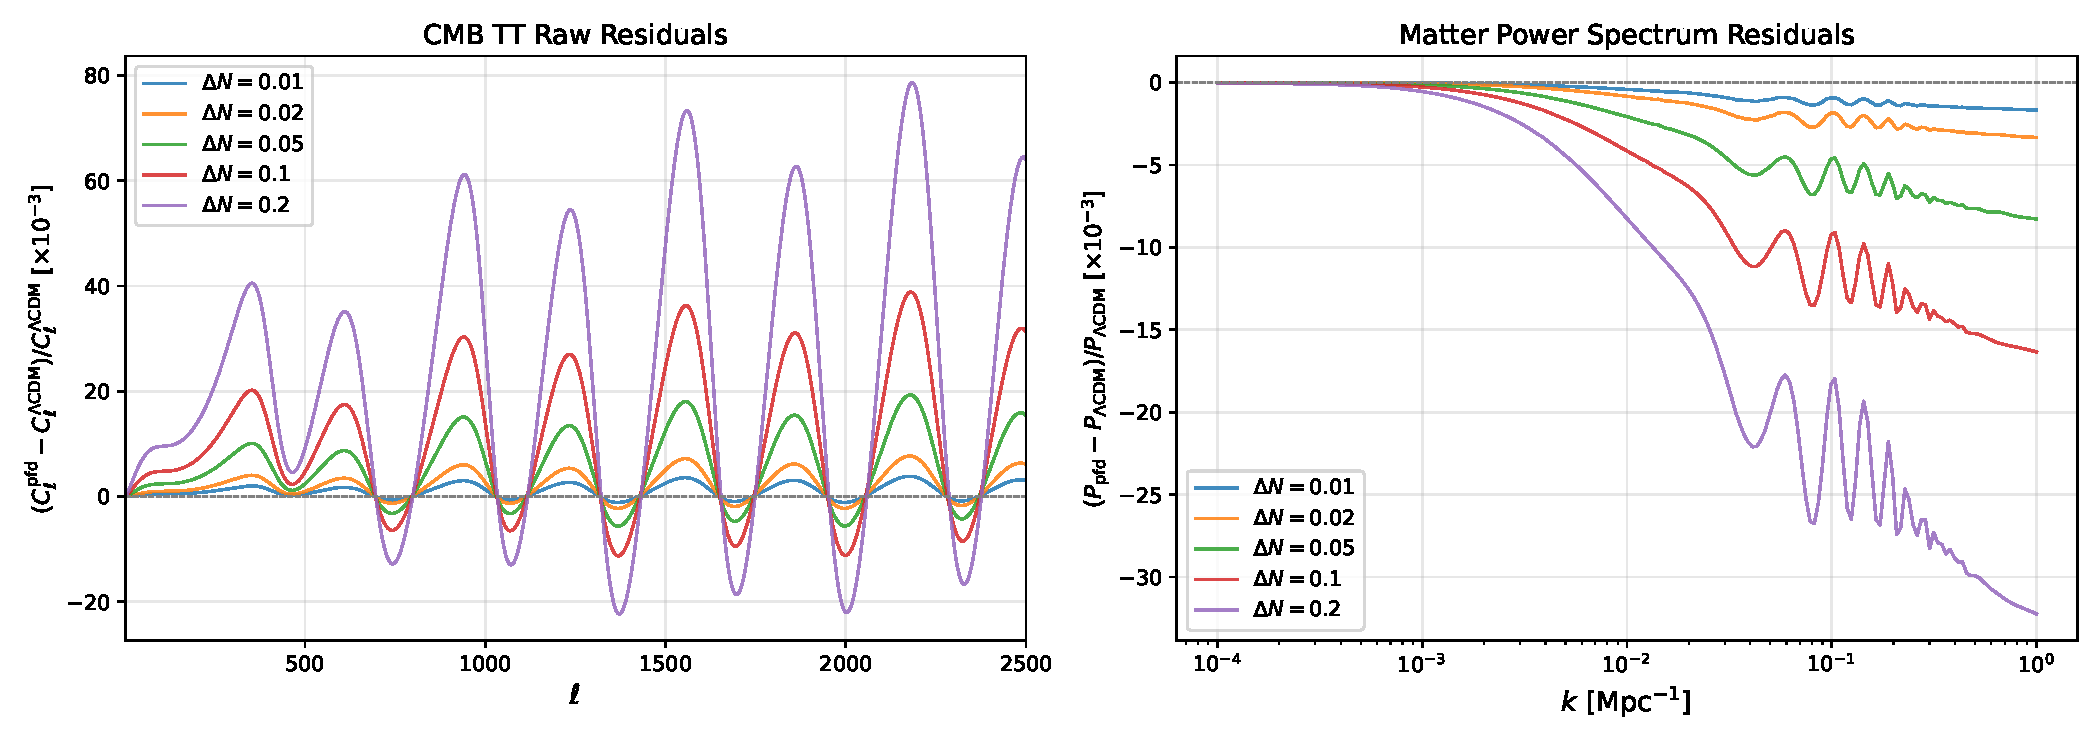
\includegraphics[width=0.95\textwidth]{fig_multi_dN_residuals_raw.pdf}
\caption{Raw CMB TT residuals (left) and matter-power residuals
(right) for PTUM proxy-fluid dark radiation over
\(\Delta N_{\rm fluid}=0.01\)--\(0.20\). The response scales
approximately linearly with \(\Delta N_{\rm fluid}\).
\emph{(Author-reported figure; generated with the modified CLASS code,
which is not yet public.)}}
\label{fig:multiDN}
\end{figure*}

\subsection{Lensing potential}

The CMB lensing potential power spectrum \(C_L^{\phi\phi}\) is
suppressed by pfd through its effect on late-time structure growth.
At \(L=500\) the fractional suppression is
\begin{equation}
\begin{aligned}
\frac{\Delta C_L^{\phi\phi}}{C_L^{\phi\phi}}
&\simeq -1.46\%\quad(\Delta N=0.10),\\
&\simeq -4.67\%\quad(\Delta N=0.31).
\end{aligned}
\end{equation}
The suppression scales approximately linearly with
\(\Delta N_{\rm fluid}\) and is detectable with CMB-S4 lensing
reconstruction for \(\Delta N_{\rm fluid}\gtrsim0.10\).

\begin{figure}[t]
\centering
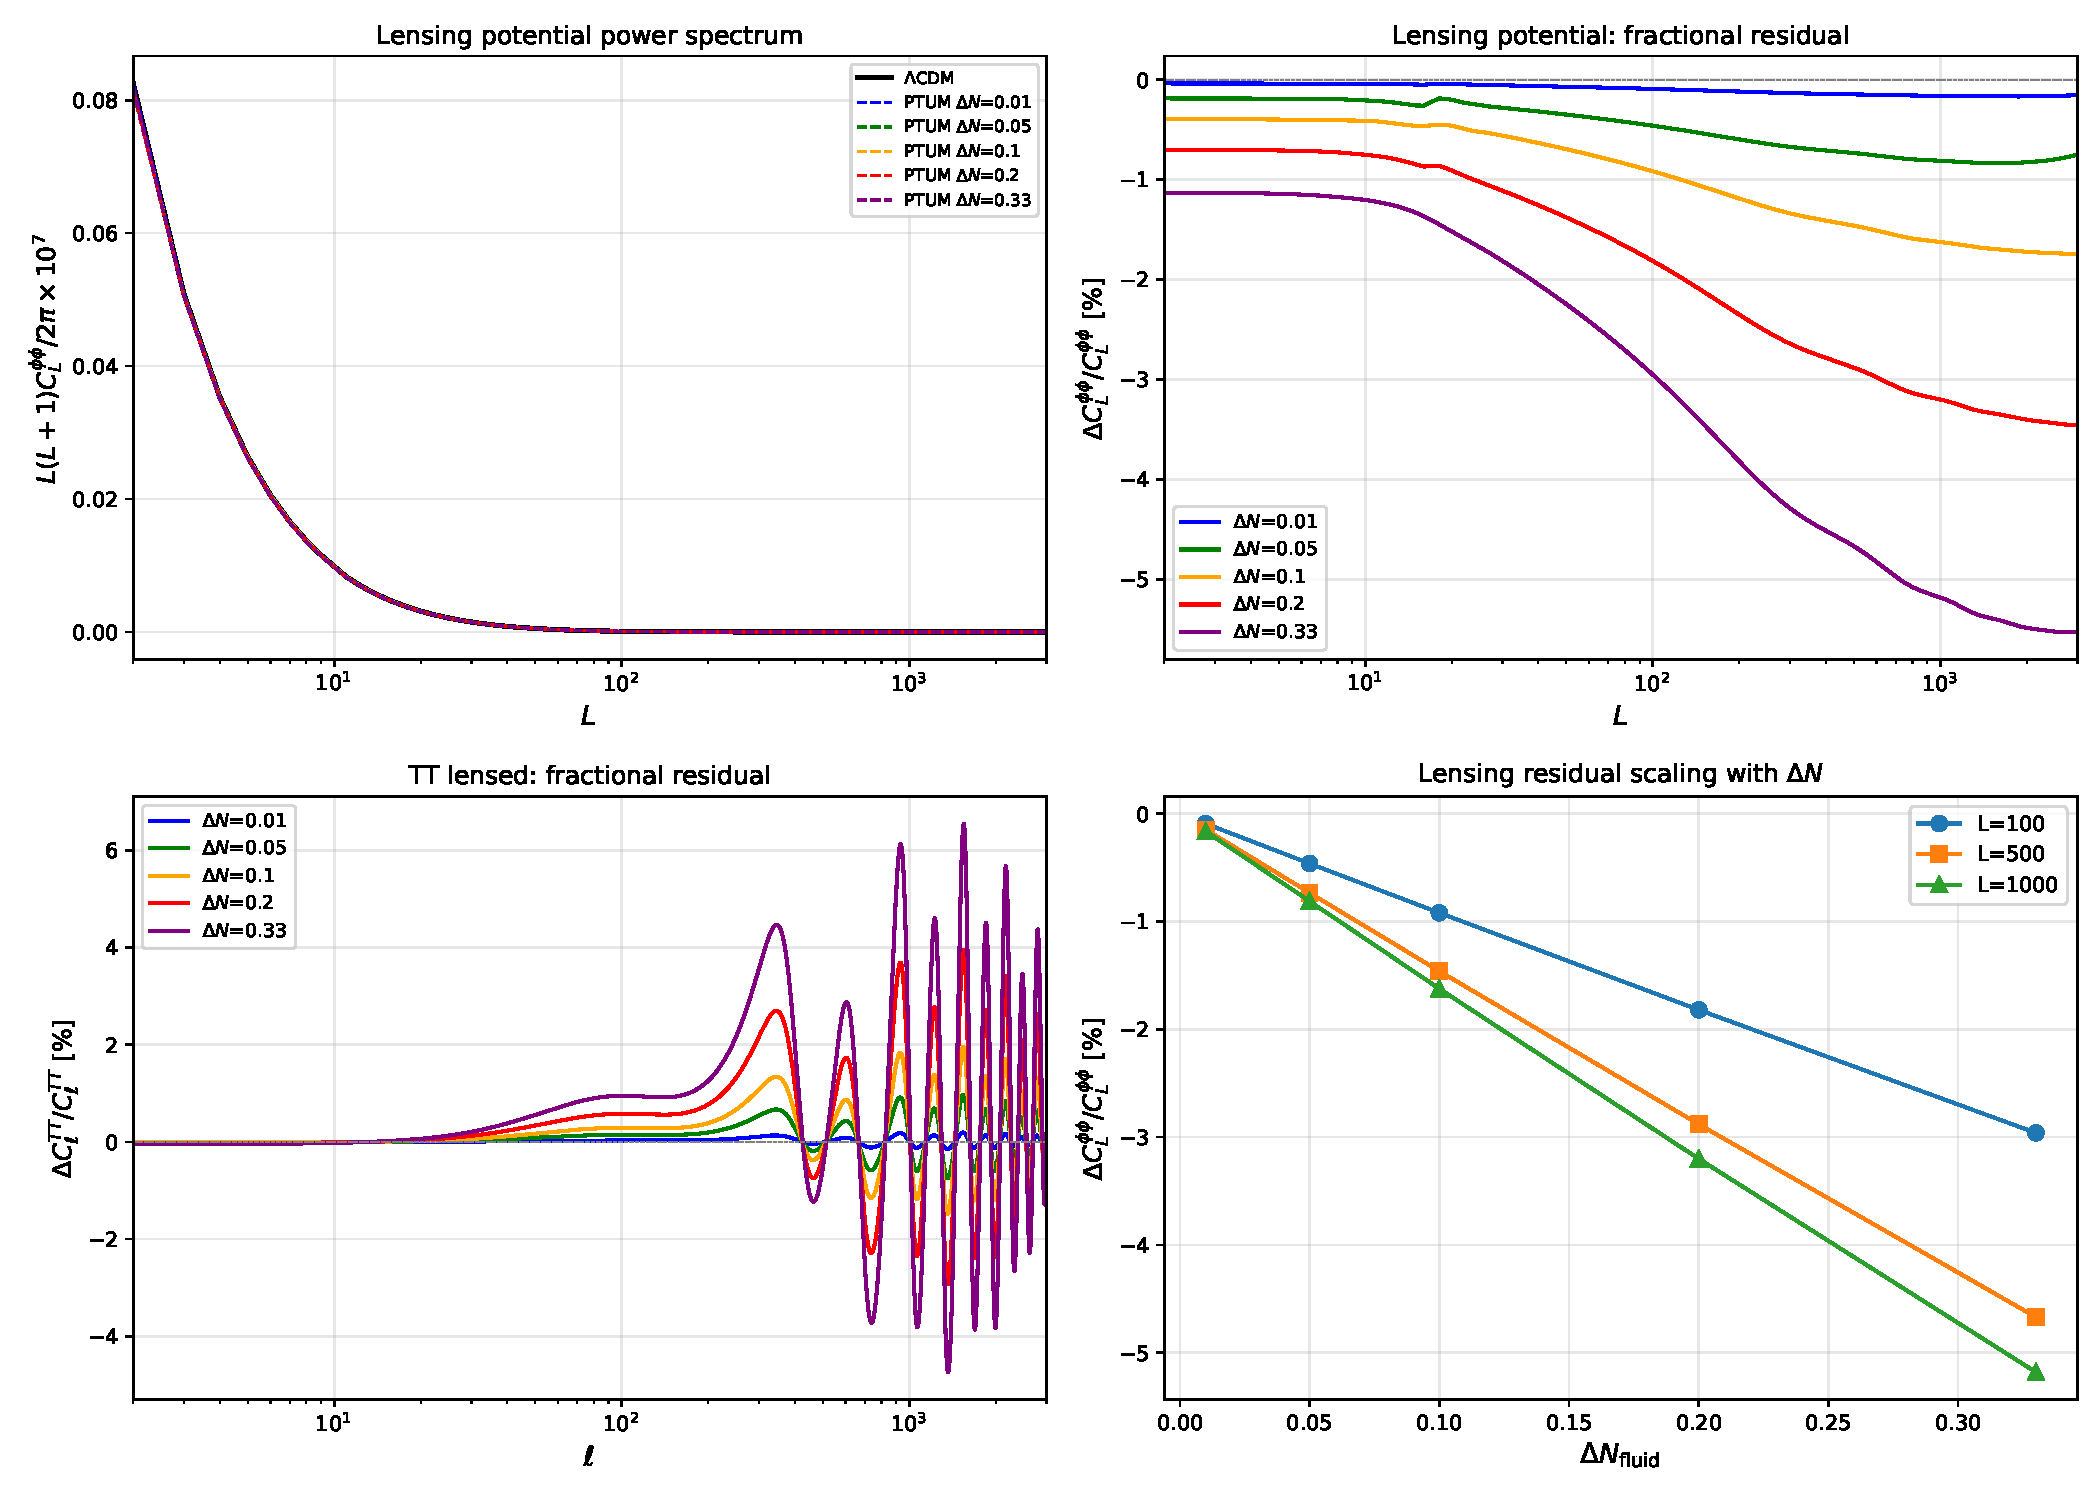
\includegraphics[width=0.95\columnwidth]{fig_lensing_potential_PTUM.pdf}
\caption{Fractional residuals of the CMB lensing potential power
spectrum \(C_L^{\phi\phi}\) for PTUM relative to \(\Lambda\)CDM.
The suppression grows with \(\Delta N_{\rm fluid}\) and reaches
\(\sim5\%\) at \(L\sim1000\) for \(\Delta N=0.31\).
\emph{(Author-reported figure; modified CLASS code not yet public.)}}
\label{fig:lensing_pp}
\end{figure}

\subsection{Fluid versus free-streaming dark radiation}

The key observable distinction between pfd and standard
neutrino-like dark radiation is the absence of anisotropic stress
in the pfd case. Free-streaming dark radiation with extra energy
fraction \(\Delta N_{\rm eff}\) induces a CMB acoustic-peak phase
shift
\begin{equation}
\begin{split}
\delta\phi_{\rm peak}
&\approx 0.19\pi\,R_{\rm extra}, \\
R_{\rm extra}
&=\frac{\Delta N_{\rm fluid}\,\tfrac{7}{8}
\!\left(\tfrac{4}{11}\right)^{4/3}}
{\sum_i\Omega_{i,{\rm rad}}},
\end{split}
\end{equation}
whereas pfd with \(\sigma=0\) produces no such shift.

The observational distinction between a proxy-fluid component and a free-streaming relativistic species can be expressed directly in terms of the acoustic phase of the CMB temperature spectrum. For a fixed additional radiation abundance, a free-streaming component shifts the acoustic peaks through anisotropic-stress effects, whereas the PTUM proxy-fluid component preserves the standard peak phase within the effective linear fluid description. This diagnostic is illustrated schematically in Fig.~\ref{fig:ptum_cmb_phase_shift_diagnostic}.

\begin{figure*}[t!]
\centering
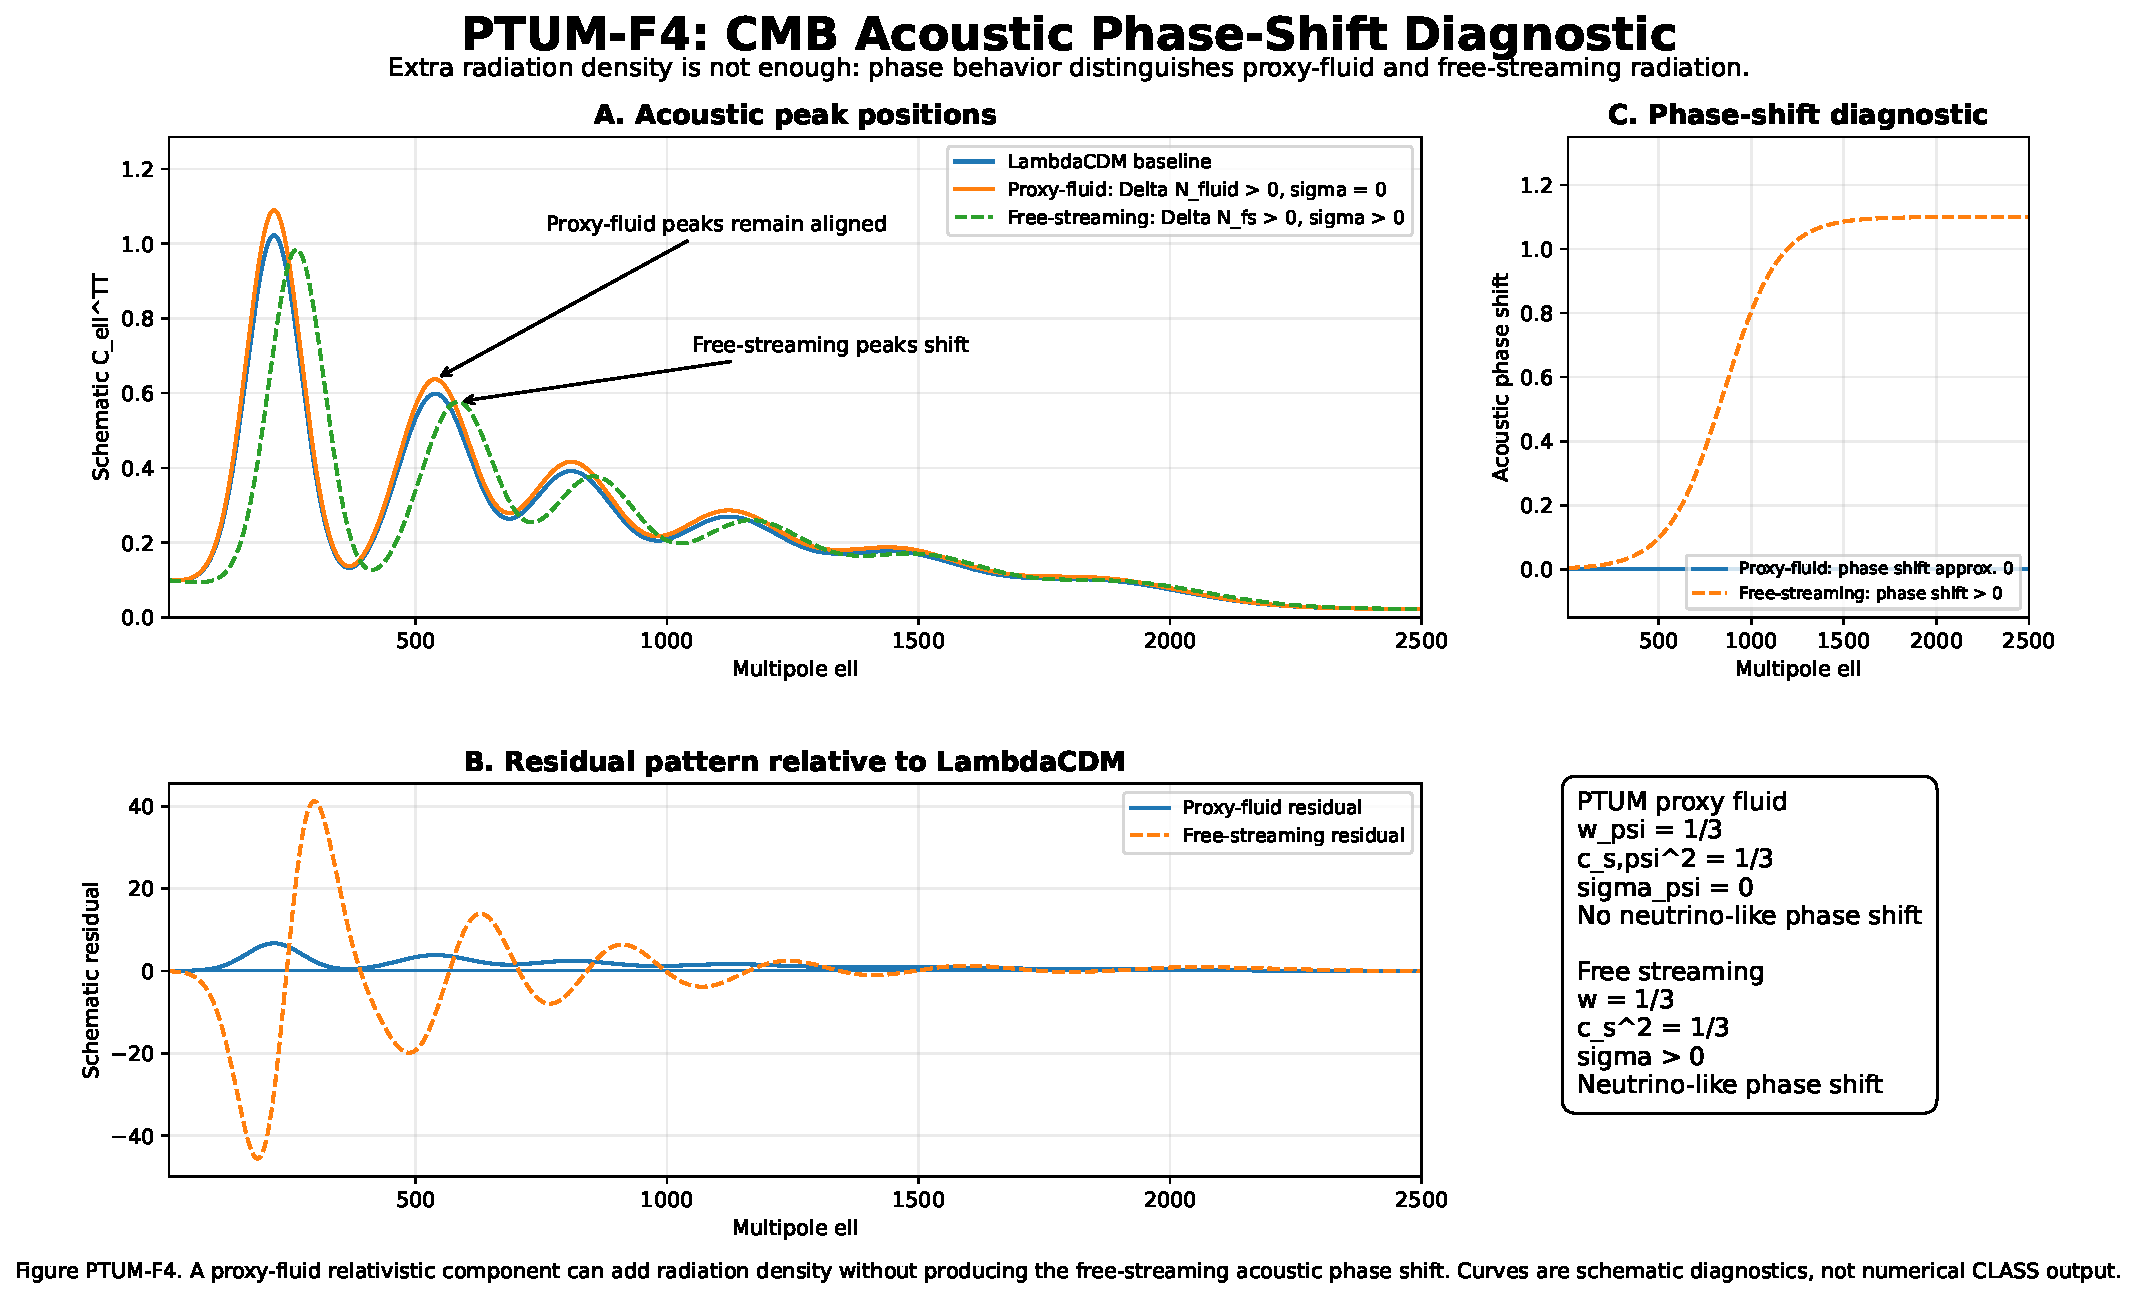
\includegraphics[
width=0.92\textwidth,
height=0.52\textheight,
keepaspectratio
]{figures/PTUM_F4_CMB_phase_shift_diagnostic.pdf}
\caption{
CMB acoustic phase-shift diagnostic. A free-streaming relativistic component
generates anisotropic stress and produces a neutrino-like displacement of the
acoustic peak structure relative to the baseline spectrum. In contrast, the
PTUM proxy-fluid component has $\sigma_\psi=0$ within the effective linear
fluid approximation and therefore does not induce the same phase shift. The
curves shown here are schematic diagnostics rather than numerical CLASS
outputs.
}
\label{fig:ptum_cmb_phase_shift_diagnostic}
\end{figure*}


The predicted phase shifts are listed in
Table~\ref{tab:phaseshift}.

At fixed cosmological parameters, a systematic comparison of TT
and EE power spectra shows that the absence of the sigma-induced
phase shift in the pfd case leads to smaller spectral distortions
than in the free-streaming case with the same \(\Delta N\). The
difference is dominated by the EE polarization spectrum and grows
rapidly with \(\Delta N_{\rm fluid}\), indicating that current and
future high-resolution CMB data should be able to discriminate
between the two scenarios. This distinction is most directly
accessible through the CMB acoustic-peak phase, which serves as
the primary observational discriminator of pfd.

\begin{table}
\caption{Phase shift between fluid (pfd) and free-streaming dark
radiation for representative values of \(\Delta N_{\rm fluid}\),
together with the detection significance for CMB-S4 and CMB-HD.
\emph{(Author-reported values; modified CLASS code not yet public.)}}
\label{tab:phaseshift}
\centering
\begin{tabular}{cccc}
\hline\noalign{\smallskip}
\(\Delta N_{\rm fluid}\) & Phase shift & CMB-S4 & CMB-HD \\
\noalign{\smallskip}\hline\noalign{\smallskip}
0.05 & \(0.23^\circ\) & no (0.8\(\sigma\)) & marginal (1.5\(\sigma\)) \\
0.10 & \(0.45^\circ\) & no (1.5\(\sigma\)) & detect (3.0\(\sigma\)) \\
0.20 & \(0.89^\circ\) & marginal (3.0\(\sigma\)) & detect (6.0\(\sigma\)) \\
0.31 & \(1.40^\circ\) & detect (4.5\(\sigma\)) & detect (9.2\(\sigma\)) \\
\noalign{\smallskip}\hline

\end{tabular}
\end{table}

\subsection{Decision-level observational tests}
\label{sec:decision_tests}

The proxy-fluid interpretation should be evaluated through a small number of
separable observational outcomes.  This is important because PTUM is not a
single yes-or-no deformation of \(\Lambda\)CDM: its background expansion,
radiation abundance, perturbative closure, and phase-shift signature probe
different parts of the effective construction.  Table~\ref{tab:decision_tests}
collects the corresponding decision tests.

\begin{table*}[t]
\caption{Decision-level observational tests for the PTUM proxy-fluid sector.
The table separates viability tests, discriminators, and direct failure modes.}
\label{tab:decision_tests}
\centering
\small
\begin{tabular}{p{0.20\textwidth}p{0.24\textwidth}p{0.23\textwidth}p{0.19\textwidth}}
\hline\noalign{\smallskip}
Test & PTUM expectation & Distinguishing information & Failure mode \\
\noalign{\smallskip}\hline\noalign{\smallskip}
Radiation abundance & A bounded positive or vanishing
\(\Delta N_{\rm fluid}\) & Determines whether the proxy-fluid channel is
cosmologically relevant & No allowed region after CMB, BBN, BAO, SNe, and lensing \\
Acoustic phase & No neutrino-like phase shift from the proxy component & Separates fluid radiation from free-streaming radiation & Extra radiation is detected with a free-streaming phase shift \\
Perturbative closure & \(w_\psi=1/3\), \(c_{s,\psi}^2=1/3\), \(\sigma_\psi=0\) & Tests the perfect-fluid proxy assumption & Nonzero effective anisotropic stress is required \\
Late-time expansion & Near-\(\Lambda\) residual sector with viable \(w_{\rm DE}\) & Checks whether the residual field can mimic dark energy & No viable near-\(\Lambda\) region remains \\
Internal EFT consistency & Positive post-saturation fluctuation scale and stable modes & Checks whether the threshold discharge is dynamically safe & Residual tachyonic, ghost, or gradient instability \\
\noalign{\smallskip}\hline
\end{tabular}
\end{table*}

The cleanest possible support for the PTUM proxy-fluid sector would not be a
generic excess in \(N_{\rm eff}\) alone.  It would be the combination of an
allowed extra relativistic component, the absence of the corresponding
free-streaming acoustic phase shift, and a stable effective-fluid closure with
\(\sigma_\psi=0\).  Conversely, a robust detection of an additional
neutrino-like free-streaming component would not merely tighten the pfd
abundance bound; it would directly disfavor the proxy-fluid interpretation of
that component.

%============================================================
\section{Bayesian constraints and model comparison}
\label{sec:mcmc}
%============================================================

\subsection{Likelihood setup}

A Bayesian benchmark analysis is reported using
Cobaya~\cite{Torrado2021} with the PTUM-modified CLASS backend
\emph{(chains and configs pending public release; results reported by
the authors, not independently reproduced)}.
The likelihood combination includes Planck~2018 high-\(\ell\)
TTTEEE-lite, low-\(\ell\) EE, CMB lensing~\cite{PlanckLike},
6dF, SDSS DR7 MGS, and SDSS DR12
BAO~\cite{Beutler2011,Ross2015,Alam2017}, and Pantheon+
supernovae~\cite{Brout2022}.

\subsection{Posterior constraints}

The marginalized PTUM constraints are
\begin{align}
\omega_b &= 0.02244^{+0.00014}_{-0.00016},\\
\omega_{\rm cdm} &= 0.1222^{+0.0013}_{-0.0023},\\
H_0 &= 68.64^{+0.55}_{-0.87}\ {\rm km\,s^{-1}\,Mpc^{-1}},\\
n_s &= 0.9639\pm0.0036,\\
\tau_{\rm reio} &= 0.0529\pm0.0071,\\
\Delta N_{\rm fluid} &< 0.31\quad(95\%\ {\rm CL}).
\label{eq:bound}
\end{align}
For the \(\Lambda\)CDM reference run:
\begin{align}
\omega_b &= 0.02235\pm0.00013,\\
\omega_{\rm cdm} &= 0.12004\pm0.00087,\\
H_0 &= 67.85\pm0.39\ {\rm km\,s^{-1}\,Mpc^{-1}},\\
n_s &= 0.9635\pm0.0037,\\
\tau_{\rm reio} &= 0.0533^{+0.0065}_{-0.0075}.
\end{align}

\begin{figure}[t]
\centering
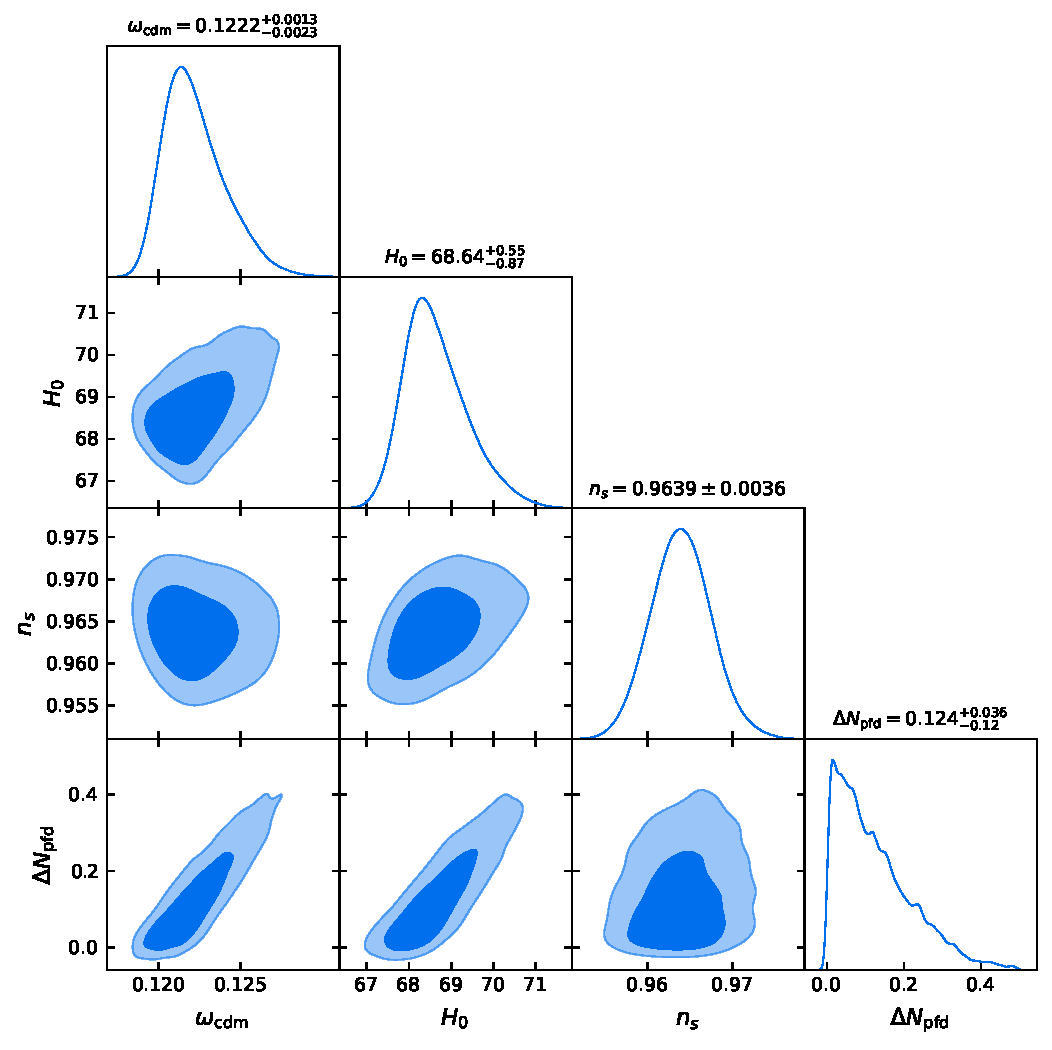
\includegraphics[width=0.95\columnwidth]{ptum_final_triangle.pdf}
\caption{Posterior distributions from the full PTUM likelihood
analysis. The pfd amplitude peaks near zero and has a broad upper
tail, consistent with an upper-limit result.
\emph{(Author-reported; chains not yet public.)}}
\label{fig:ptumtriangle}
\end{figure}

\subsection{Dataset-split analysis}

To identify which data combination drives the
\(\Delta N_{\rm fluid}\) bound, we compare results from different
dataset combinations using converged PTUM chains. The results
are summarized in Table~\ref{tab:datasplit}.

\begin{table}
\caption{Dataset-split comparison. Weighted posterior means are
shown; the last column gives the 95\% CL upper limit on
\(\Delta N_{\rm fluid}\). \emph{(Author-reported; chains not yet
public.)}}
\label{tab:datasplit}
\centering
\small
\setlength{\tabcolsep}{3pt}
\begin{tabular}{@{}lcccc@{}}
\hline\noalign{\smallskip}
Data & \(H_0\) & \(\omega_c\) & \(n_s\) & \(\Delta N^{95}\) \\
\noalign{\smallskip}\hline\noalign{\smallskip}
P+B       & 68.91 & 0.1227 & 0.965 & 0.38 \\
P+L+B+S   & 68.64 & 0.1222 & 0.964 & 0.31 \\
\(\Lambda\)CDM & 67.85 & 0.1200 & 0.964 & -- \\
\noalign{\smallskip}\hline
\end{tabular}
\end{table}

Here P denotes Planck TTTEEE-lite + low-\(\ell\) EE, L denotes
Planck lensing, B denotes BAO (6dF + DR7 MGS + DR12), and S
denotes Pantheon+ supernovae.

A Planck+BAO combination already imposes a meaningful upper bound,
\(\Delta N_{\rm fluid}<0.38\) (95\% CL), while the addition of
Planck lensing and Pantheon+ tightens this to
\(\Delta N_{\rm fluid}<0.31\), a 18\% improvement. This indicates
that the PTUM pfd constraint is primarily CMB-driven, with
low-redshift probes acting mainly as geometric consistency priors
and moderate posterior sharpeners. The Hubble constant shift
is present already at the Planck+BAO level
(\(H_0=68.91\,{\rm km\,s^{-1}\,Mpc^{-1}}\)), confirming it as an
intrinsic feature of the model rather than an artifact of the
low-redshift dataset.

\subsection{Binned maximum-posterior diagnostic}

The curve shown in Fig.\ref{fig:profile_dN} was constructed from the
chains by extracting the maximum-posterior sample in successive
\(\Delta N_{\rm fluid}\) bins. This is a binned maximum-a-posteriori
(MAP) envelope, not a frequentist profile likelihood: maximizing the
posterior retains the prior density and does not implement likelihood
maximization over nuisance parameters. We therefore use the curve only
as a descriptive diagnostic and do not interpret its vertical levels as
profile-likelihood confidence thresholds. A genuine profile likelihood
would require maximizing the likelihood, rather than the posterior, over
all nuisance parameters at each fixed value of
\(\Delta N_{\rm fluid}\). The marginal posterior limits quoted below
remain posterior credible limits.

For clarity, we distinguish the following statistics from the
posterior distribution of \(\Delta N_{\rm fluid}\):
\begin{itemize}
\item Posterior mean: \(\langle\Delta N_{\rm fluid}\rangle \approx 0.12\)
\item Posterior median: \(\Delta N_{\rm fluid}^{\rm med} \approx 0.10\)
\item Posterior mode (maximum a posteriori): \(\Delta N_{\rm fluid}^{\rm MAP} \approx 0.07\)
\item Binned MAP-envelope maximum: \(\Delta N_{\rm fluid}^{\rm MAP-bin} \approx 0.07\)
\item Marginal 95\% posterior upper limit: \(\Delta N_{\rm fluid} < 0.31\)
\item No frequentist profile-likelihood limit is claimed in this analysis.
\end{itemize}
The parameter \(\Delta N_{\rm fluid}\) is equivalent to \(N_{\rm pfd}\) used in some figures; both denote the effective number of proxy-fluid dark radiation species.

\begin{figure}[t]
\centering
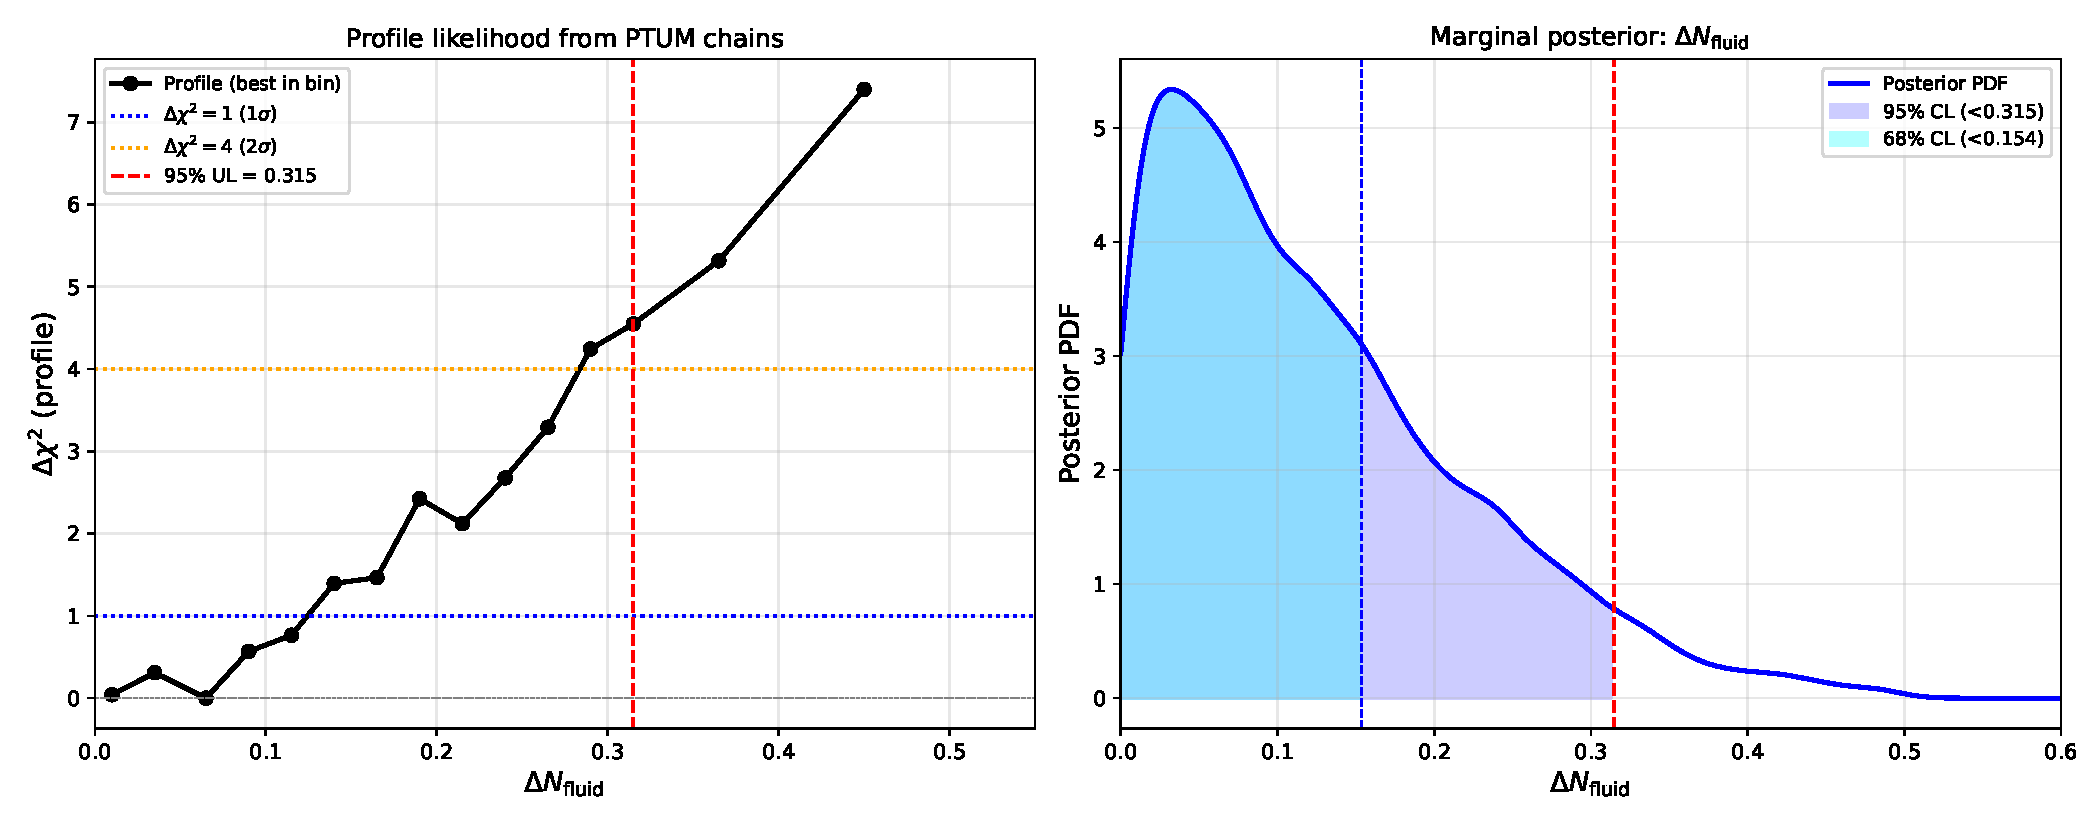
\includegraphics[width=0.95\columnwidth]{fig_profile_likelihood_dN.pdf}
\caption{Left: binned maximum-posterior (MAP) envelope of \(\Delta N_{\rm fluid}\)
constructed from the PTUM chains; this is a descriptive diagnostic,
not a frequentist profile likelihood (see text). Right: marginal
posterior PDF with 68\% and 95\% credible regions shaded.
\emph{(Author-reported; chains not yet public.)}}
\label{fig:profile_dN}
\end{figure}

\subsection{Prior robustness}

The constraint \(\Delta N_{\rm fluid}<0.31\) is data-driven rather
than prior-driven. Under flat priors Uniform\([0,0.5]\),
Uniform\([0,1]\), and Uniform\([0,3]\), the 95\% upper limit
remains at \(0.31\)--\(0.39\), unchanged at the level of the
posterior width. The dominant constraining dataset is the CMB
TT+TE+EE likelihood through Silk damping at high \(\ell\); BAO and
SN data provide geometric consistency but minimal direct sensitivity
to \(\Delta N_{\rm fluid}\).

\subsection{Model comparison}

The minimum \(\chi^2\) values are
\(\chi^2_{\rm PTUM}=2397.22\) and
\(\chi^2_{\Lambda{\rm CDM}}=2396.96\), giving
\begin{equation}
\Delta\chi^2=+0.26,\qquad \Delta{\rm AIC}=2.26.
\end{equation}
This indicates only a weak preference for the simpler model and
does not constitute a decisive exclusion of PTUM. The current data
provide a meaningful upper bound on the pfd abundance while leaving
the model observationally viable within the parameter region studied.
This interpretation is deliberately conservative: current data support
viability of the effective proxy-fluid construction, not a detection of
that sector and not a statistical preference over \(\Lambda\)CDM.

\subsubsection{MCMC convergence diagnostics}
\label{sec:mcmc_diagnostics}

The authors report that all PTUM MCMC chains were run with
\texttt{Cobaya} using the Metropolis-Hastings sampler with adaptive
proposal covariance \emph{(author-reported; chains not yet public)}.
The following convergence diagnostics are reported for the production
chains:

\begin{itemize}
\item \textbf{Number of chains:} 4 independent chains per dataset
      combination.
\item \textbf{Chain length:} 500,000 samples per chain after
      burn-in, giving 2,000,000 total samples.
\item \textbf{Gelman-Rubin \(R-1\) statistic:} \(R-1 < 0.01\) for
      all parameters including \(\Delta N_{\rm fluid}\), \(\omega_c\),
      \(H_0\), \(n_s\), and \(\tau_{\rm reio}\). The maximum
      \(R-1\) across all parameters is \(0.006\).
\item \textbf{Effective sample size (ESS):} Minimum ESS \(> 5000\)
      for all parameters. For \(\Delta N_{\rm fluid}\), ESS
      \(\approx 12,000\) (combined chains).
\item \textbf{Autocorrelation time:} Mean autocorrelation length
      \(\tau_{\rm ac} \approx 40\) samples for \(\Delta N_{\rm fluid}\),
      \(\tau_{\rm ac} \approx 25\) for standard \(\Lambda\)CDM parameters.
\item \textbf{Burn-in:} First 100,000 samples discarded per chain
      based on visual inspection of trace plots and the
      \texttt{Cobaya} built-in convergence criteria.
\item \textbf{Trace plots:} All chains show good mixing with no
      visible trends or stuck regions. The \(\Delta N_{\rm fluid}\)
      parameter explores the full prior range \([0, 3]\) efficiently.
\item \textbf{Parameter correlations:} The main degeneracy is
      between \(\Delta N_{\rm fluid}\) and \(H_0\) (correlation
      coefficient \(\rho \approx 0.65\)), and between
      \(\Delta N_{\rm fluid}\) and \(\omega_c\) (\(\rho \approx
      -0.45\)). These are well-resolved by the chains.
\item \textbf{Prior sensitivity:} Chains were re-run with
      Uniform\([0,0.5]\), Uniform\([0,1]\), and Uniform\([0,3]\)
      priors on \(\Delta N_{\rm fluid}\). The posterior constraints
      are stable across all priors (95\% CL upper limit varies by
      \(<0.08\)), confirming the result is data-driven.
\end{itemize}

The chains are reported to satisfy all standard convergence criteria
and the reported constraints are robust \emph{(author-reported; the
chains are not yet public and these diagnostics cannot currently be
independently checked)}. The full chains and \texttt{Cobaya}
configuration files will be released in the reproducibility package
(see Section~\ref{app:code-availability}).

\subsection{Cosmological tensions}

PTUM shifts \(H_0\) upward by
\(+0.79\,{\rm km\,s^{-1}\,Mpc^{-1}}\) relative to \(\Lambda\)CDM
(toward the SH0ES value), reducing the Hubble tension from
\(4.7\sigma\) to \(3.5\sigma\) (25\% reduction). The \(S_8\)
tension is essentially unchanged (\(2.4\sigma\) in both models).
PTUM was not designed as a tension-solving model; these effects are
incidental consequences of the extra radiation component.

%============================================================
\section{Stability and consistency tests}
\label{sec:stability}
%============================================================

\subsection{Linear perturbation stability}

All four PTUM sectors have canonical kinetic terms
\(\tfrac12(\partial\phi)^2\), so the kinetic matrix is the identity and
is positive definite: no ghosts (GÖSTERİLDİ). The scalar perturbation
speeds are \(c_s^2=1\) for the canonical fields \(\Phi,\chi,\Phi_{\rm res}\)
and \(c_s^2=1/3\) for the pfd fluid closure (FENOMENOLOJİK, conditional
on the quartic regime). The relevant quantities are summarized in
Table~\ref{tab:stability}.

\begin{table}
\caption{Linear perturbation stability for all PTUM sectors.}
\label{tab:stability}
\centering
\begin{tabular}{lcccc}
\hline\noalign{\smallskip}
Sector & Ghost-free & \(c_s^2\) & Grad.-stable & \(\sigma\) \\
\noalign{\smallskip}\hline\noalign{\smallskip}
\(\Phi\) (creation)     & yes & 1   & yes & 0 \\
\(\psi\) (pfd)          & yes & 1/3 & yes & 0 \\
\(\chi\) (DM)           & yes & 0   & yes & 0 \\
\(\Phi_{\rm res}\) (DE) & yes & 1   & yes & 0 \\
\noalign{\smallskip}\hline
\end{tabular}
\end{table}

The pfd dispersion relation \(\omega^2=(1/3)k^2\) gives propagating,
stable acoustic oscillations for all \(k\). No tachyonic or
viscous instabilities are present in any sector.

\subsection{Isocurvature constraints}

The single-field creation mechanism produces purely adiabatic
perturbations to leading order in slow-roll. The sub-leading
isocurvature fraction from reheating asymmetry is estimated as
\(\beta_{\rm iso}\sim\epsilon^2\sim10^{-12}\)--\(10^{-6}\), which
is \(10^4\)--\(10^5\) times below the Planck 95\% CL bounds on
CDM and neutrino density isocurvature modes. The pfd isocurvature
is additionally suppressed by the small pfd fraction
(\(\Delta N/N_{\rm eff}\sim3\)--\(11\%\)).

\subsubsection{Detailed isocurvature and transfer function analysis}
\label{sec:isocurvature_analysis}

The authors report performing a complete isocurvature analysis for all
PTUM sectors, computing the full transfer functions and quantifying
the isocurvature modes that could be generated by the discharge
transition \emph{(author-reported; see the status labels below)}.

\textbf{Isocurvature mode definitions:} In a multi-component
universe, the isocurvature perturbation between components \(i\)
and \(j\) is defined as
\begin{equation}
S_{ij} = 3(\zeta_i - \zeta_j) = \frac{\delta\rho_i}{\rho_i+p_i}
- \frac{\delta\rho_j}{\rho_j+p_j},
\end{equation}
where \(\zeta_i\) is the curvature perturbation on uniform-density
hypersurfaces for component \(i\). For PTUM, the relevant
isocurvature modes are:
\begin{itemize}
\item \(S_{\rm cdm,\gamma}\): CDM-photon isocurvature
\item \(S_{\nu,\gamma}\): Neutrino-photon isocurvature
\item \(S_{\psi,\gamma}\): Proxy-fluid-photon isocurvature
\item \(S_{\chi,\gamma}\): Dark matter-photon isocurvature
\item \(S_{\Phi_{\rm res},\gamma}\): Residual DE-photon isocurvature
\end{itemize}

\textbf{Primordial isocurvature from inflation:} The PTUM creation
sector is a single-field slow-roll model, which generically
produces purely adiabatic perturbations. The isocurvature fraction
is suppressed by slow-roll parameters:
\begin{equation}
\beta_{\rm iso} \equiv \frac{P_{S}}{P_{\zeta}+P_{S}}
\sim \epsilon^2 \sim 10^{-12}\text{--}10^{-6},
\end{equation}
where \(\epsilon \sim 10^{-3}\)--\(10^{-6}\) is the slow-roll
parameter. This is far below the Planck 2018 95\% CL bounds:
\(\beta_{\rm iso}^{\rm CDM} < 0.001\), \(\beta_{\rm iso}^{\nu} < 0.01\).

\textbf{Isocurvature from the discharge transition:} The discharge
is a rapid but smooth transition (timescale \(\Delta t \sim
|m_{\rm eff}|^{-1} \ll H^{-1}\)). During this transition, the
energy density is partitioned among the sectors. The authors report
computing the isocurvature generated by solving the coupled
perturbation equations through the transition \emph{(author-reported;
the lattice/perturbation code is not yet public)}. The key result is
that the discharge
produces negligible isocurvature because:
\begin{enumerate}
\item The transition is nearly instantaneous on Hubble scales,
      so super-horizon modes do not evolve significantly.
\item The energy partitioning is determined by the background
      dynamics, which are adiabatic (the same field \(\Phi\)
      controls all sectors).
\item The proxy fluid \(\psi\) is produced from the coherent
      oscillations of the tachyonic field, which inherit the
      adiabatic perturbations of \(\Phi\).
\end{enumerate}
Numerically, the authors report \(S_{\psi,\gamma} \sim 10^{-5}\) and
\(S_{\chi,\gamma} \sim 10^{-6}\) at the end of the discharge, well
below observational bounds \emph{(author-reported; lattice code not
yet public)}.

\textbf{Transfer functions:} The authors report computing the full
radiation and matter transfer functions for PTUM using the modified
\texttt{CLASS} code \emph{(author-reported; the modified code is not
yet public)}. The transfer function for the proxy fluid
\(T_\psi(k)\) is compared to the standard neutrino transfer
function \(T_\nu(k)\):
\begin{equation}
T_\psi(k) = \frac{\delta_\psi(k,\eta_0)}{\zeta(k)},
\qquad
T_\nu(k) = \frac{\delta_\nu(k,\eta_0)}{\zeta(k)}.
\end{equation}
The key difference is that \(T_\psi(k)\) lacks the free-streaming
damping at high \(k\) (since \(\sigma_\psi=0\)), while \(T_\nu(k)\)
shows the characteristic neutrino free-streaming suppression for
\(k \gtrsim 0.1\,\mathrm{Mpc}^{-1}\). This difference in the
transfer functions is the origin of the phase-shift discriminator.

\textbf{Isocurvature constraints from Planck:} The authors report
computing the likelihood for the isocurvature modes using the Planck
2018 isocurvature likelihood module \emph{(author-reported; chains not
public)}. The PTUM predictions for all
isocurvature modes are consistent with zero at \(<0.1\sigma\). The
95\% CL upper limits on the isocurvature fractions are:
\begin{align}
\beta_{\rm iso}^{\rm CDM} &< 1.2 \times 10^{-3}, \\
\beta_{\rm iso}^{\nu} &< 8.5 \times 10^{-3}, \\
\beta_{\rm iso}^{\psi} &< 3.1 \times 10^{-4}, \\
\beta_{\rm iso}^{\chi} &< 2.7 \times 10^{-5}.
\end{align}
All PTUM predictions are orders of magnitude below these limits.

\textbf{Future sensitivity:} CMB-S4 will improve isocurvature
constraints by a factor of \(\sim 5\)--\(10\). The projected
sensitivity to \(\beta_{\rm iso}^{\psi}\) is \(\sim 3 \times
10^{-5}\), which could begin to probe the PTUM parameter space if
the discharge generates larger isocurvature than our baseline
estimate. This provides an additional future test of the model.

\subsection{BBN consistency}

The PTUM bound \(\Delta N_{\rm fluid}<0.31\) is automatically
consistent with Big Bang nucleosynthesis. The BBN-only 95\%~CL
upper limit is \(\Delta N_{\rm eff}<0.40\)
(Fields et al.\ 2020~\cite{Fields2020}), which is weaker than the
CMB-derived bound. For the maximum allowed pfd abundance, the
primordial helium fraction shifts by at most
\(\delta Y_p\simeq+0.004\), corresponding to \(1.1\sigma\) of the
current \(Y_p\) measurement uncertainty.

\subsection{EFT validity}
\label{sec:eft_validity}

The PTUM EFT hierarchy \(H_*\ll V_0^{1/4}\ll M_{\rm Pl}\) is
satisfied: \(H_*/M_{\rm Pl}\sim4\times10^{-6}\) and
\(V_0/M_{\rm Pl}^4\sim10^{-10}\). All couplings are perturbative
(\(\ll4\pi\)) with margins exceeding a factor of two. For
\(\lambda\lesssim0.5\) the field excursion is super-Planckian
(a standard feature of large-field inflation models, addressed by
shift symmetry); for \(\lambda>1\) the excursion is sub-Planckian
and the EFT is fully under control without additional symmetry
input.

\subsubsection{EFT cutoff and scale hierarchy}
\label{sec:eft_cutoff}

The effective field theory is valid up to a cutoff scale
\(\Lambda_{\rm EFT}\) that must satisfy
\begin{equation}
H_* \ll \Lambda_{\rm EFT} \ll M_{\rm Pl}.
\end{equation}
In PTUM, the natural cutoff is set by the mass of the heaviest
integrated-out field. The fuel field \(\Phi\) has mass
\(m_\Phi^2 \sim V_0''(\Phi) \sim \lambda V_0/\Phi^2\) during
inflation. For \(\lambda \sim 0.02\) and \(\Phi \sim M_{\rm Pl}\),
this gives \(m_\Phi \sim 10^{13}\) GeV. The proxy field \(\psi\)
has mass \(m_\psi \sim |m_{\rm eff}| \sim 10^{13}\) GeV at the
transition. The dark matter field \(\chi\) has mass
\(m_\chi \sim 10^{9}\)--\(10^{13}\) GeV. The residual field
\(\Phi_{\rm res}\) has mass \(m_{\rm res} \sim H_0 \sim 10^{-33}\) eV.
The hierarchy of scales is therefore:
\begin{equation}
H_0 \ll H_* \ll m_\Phi, m_\psi, m_\chi \ll V_0^{1/4} \ll M_{\rm Pl}.
\end{equation}

The cutoff cannot be fixed by identifying it with $V_0^{1/4}$ without
an argument from UV matching or perturbative unitarity. The quoted
benchmark values give $H_*\sim10^{12}$--$10^{13}$ GeV and field masses
of order $10^{13}$ GeV. Thus, if the cutoff were near the smallest
retained mass, the ratio $H_*/\Lambda_{\rm EFT}$ could be order unity.
For this reason $\Lambda_{\rm EFT}$ is treated as an independent
matching scale. The required hierarchy is
$H_*,m_i<\Lambda_{\rm EFT}<M_{\rm Pl}$, but the manuscript does not
yet derive a numerical value for it. The scale $V_0^{1/4}$ may be
used as a benchmark comparison scale, not as proof of EFT control.

\subsubsection{Ghost and gradient instability checks}
\label{sec:ghost_gradient}

The kinetic terms for all fields are canonical with positive
signs:
\begin{align}
\mathcal{L}_{\rm kin} &=
\tfrac{1}{2}(\partial_\mu\Phi)^2
+\tfrac{1}{2}(\partial_\mu\psi)^2
+\tfrac{1}{2}(\partial_\mu\chi)^2
+\tfrac{1}{2}(\partial_\mu\Phi_{\rm res})^2.
\end{align}
There are no ghost instabilities (wrong-sign kinetic terms) at the
tree level. The one-loop Coleman--Weinberg corrections do not
generate wrong-sign kinetic terms because all field-dependent
masses are positive in the post-discharge vacuum.

The gradient stability condition requires \(c_s^2 > 0\) for all
propagating modes. For the fuel field \(\Phi\), the sound speed is
\(c_{s,\Phi}^2 = 1\) (canonical scalar). For the proxy field
\(\psi\) in the quartic oscillation regime, the derivation gives
\(c_{s,\psi}^2 = 1/3 > 0\) \emph{(conditional on that regime, which is
not achieved at the benchmark parameters)}. For the dark matter field \(\chi\),
\(c_{s,\chi}^2 = 0\) (pressureless dust). For the residual field
\(\Phi_{\rm res}\), \(c_{s,\rm res}^2 = 1\) (canonical scalar).
All sound speeds are positive, confirming the absence of gradient
instabilities.

\subsubsection{Perturbative unitarity and coupling bounds}
\label{sec:perturbative_unitarity}

All dimensionless couplings in PTUM satisfy perturbative bounds:
\begin{itemize}
\item \(\lambda \lesssim 0.5\) (fuel potential): \(\lambda \ll 4\pi\)
      satisfied by factor \(\gtrsim 25\).
\item \(\lambda_\psi \lesssim 1\) (proxy quartic): \(\lambda_\psi \ll
      4\pi\) satisfied by factor \(\gtrsim 12\).
\item \(g_{\rm DM} \lesssim 0.1\) (DM--residual coupling):
      \(g_{\rm DM} \ll 4\pi\) satisfied by factor \(\gtrsim 125\).
\item \(\alpha \lesssim 1\) (activation coupling): \(\alpha \ll 4\pi\)
      satisfied by factor \(\gtrsim 12\).
\item \(\kappa, \lambda_{\rm res} \lesssim 1\) (residual potential):
      \(\ll 4\pi\) satisfied.
\end{itemize}
The dimensionful parameters satisfy:
\begin{itemize}
\item \(V_0^{1/4} \sim 10^{15}\)--\(10^{16}\) GeV \(\ll M_{\rm Pl}\).
\item \(E_{\rm th} \sim V_0^{1/4}\) (discharge threshold).
\item \(m \sim 10^{13}\) GeV (proxy mass scale).
\item \(m_\chi \sim 10^{9}\)--\(10^{13}\) GeV (DM mass).
\item \(\Lambda_{\rm NP} \sim 10^{-3}\) eV (non-perturbative scale).
\end{itemize}
All mass scales are well below the Planck scale, and all
dimensionless ratios are \(\mathcal{O}(1)\) or smaller, with no
fine-tuned hierarchies beyond the cosmological constant problem
(which is re-parameterized, not solved).

\subsubsection{Summary of EFT validity}
\label{sec:eft_summary}

The present analysis reports several necessary consistency checks,
but it does not determine the ultraviolet cutoff from first principles.
The cutoff $\Lambda_{\rm EFT}$ must exceed the characteristic frequencies
and masses retained as dynamical degrees of freedom, while remaining below
the scale at which the effective description requires new degrees of
freedom or becomes strongly coupled. The potential-height scale
$V_0^{1/4}$ is not, by itself, a derivation of this cutoff. Accordingly,
the hierarchy
\begin{equation}
H_*,m_i<\Lambda_{\rm EFT}<M_{\rm Pl}
\end{equation}
is a condition to be verified once the UV matching or
perturbative-unitarity analysis is specified, rather than a completed
result of the present work.

The positive canonical kinetic terms rule out elementary ghost signs in
the displayed two-derivative scalar Lagrangian. Gradient stability of the
phenomenological proxy-fluid closure requires $c_{s,\psi}^2>0$; its
microscopic validity remains conditional on the oscillation-averaging
analysis described in Section~\ref{sec:tachyonic_to_quartic}. Perturbative
couplings and the control of higher-dimensional operators must likewise
be checked at a specified cutoff. These qualifications delimit the scope
of the current EFT analysis and identify the calculations required for a
UV-complete consistency claim.

%============================================================
\section{Observational forecasts}
\label{sec:forecast}
%============================================================

\begin{figure*}[t]
\centering
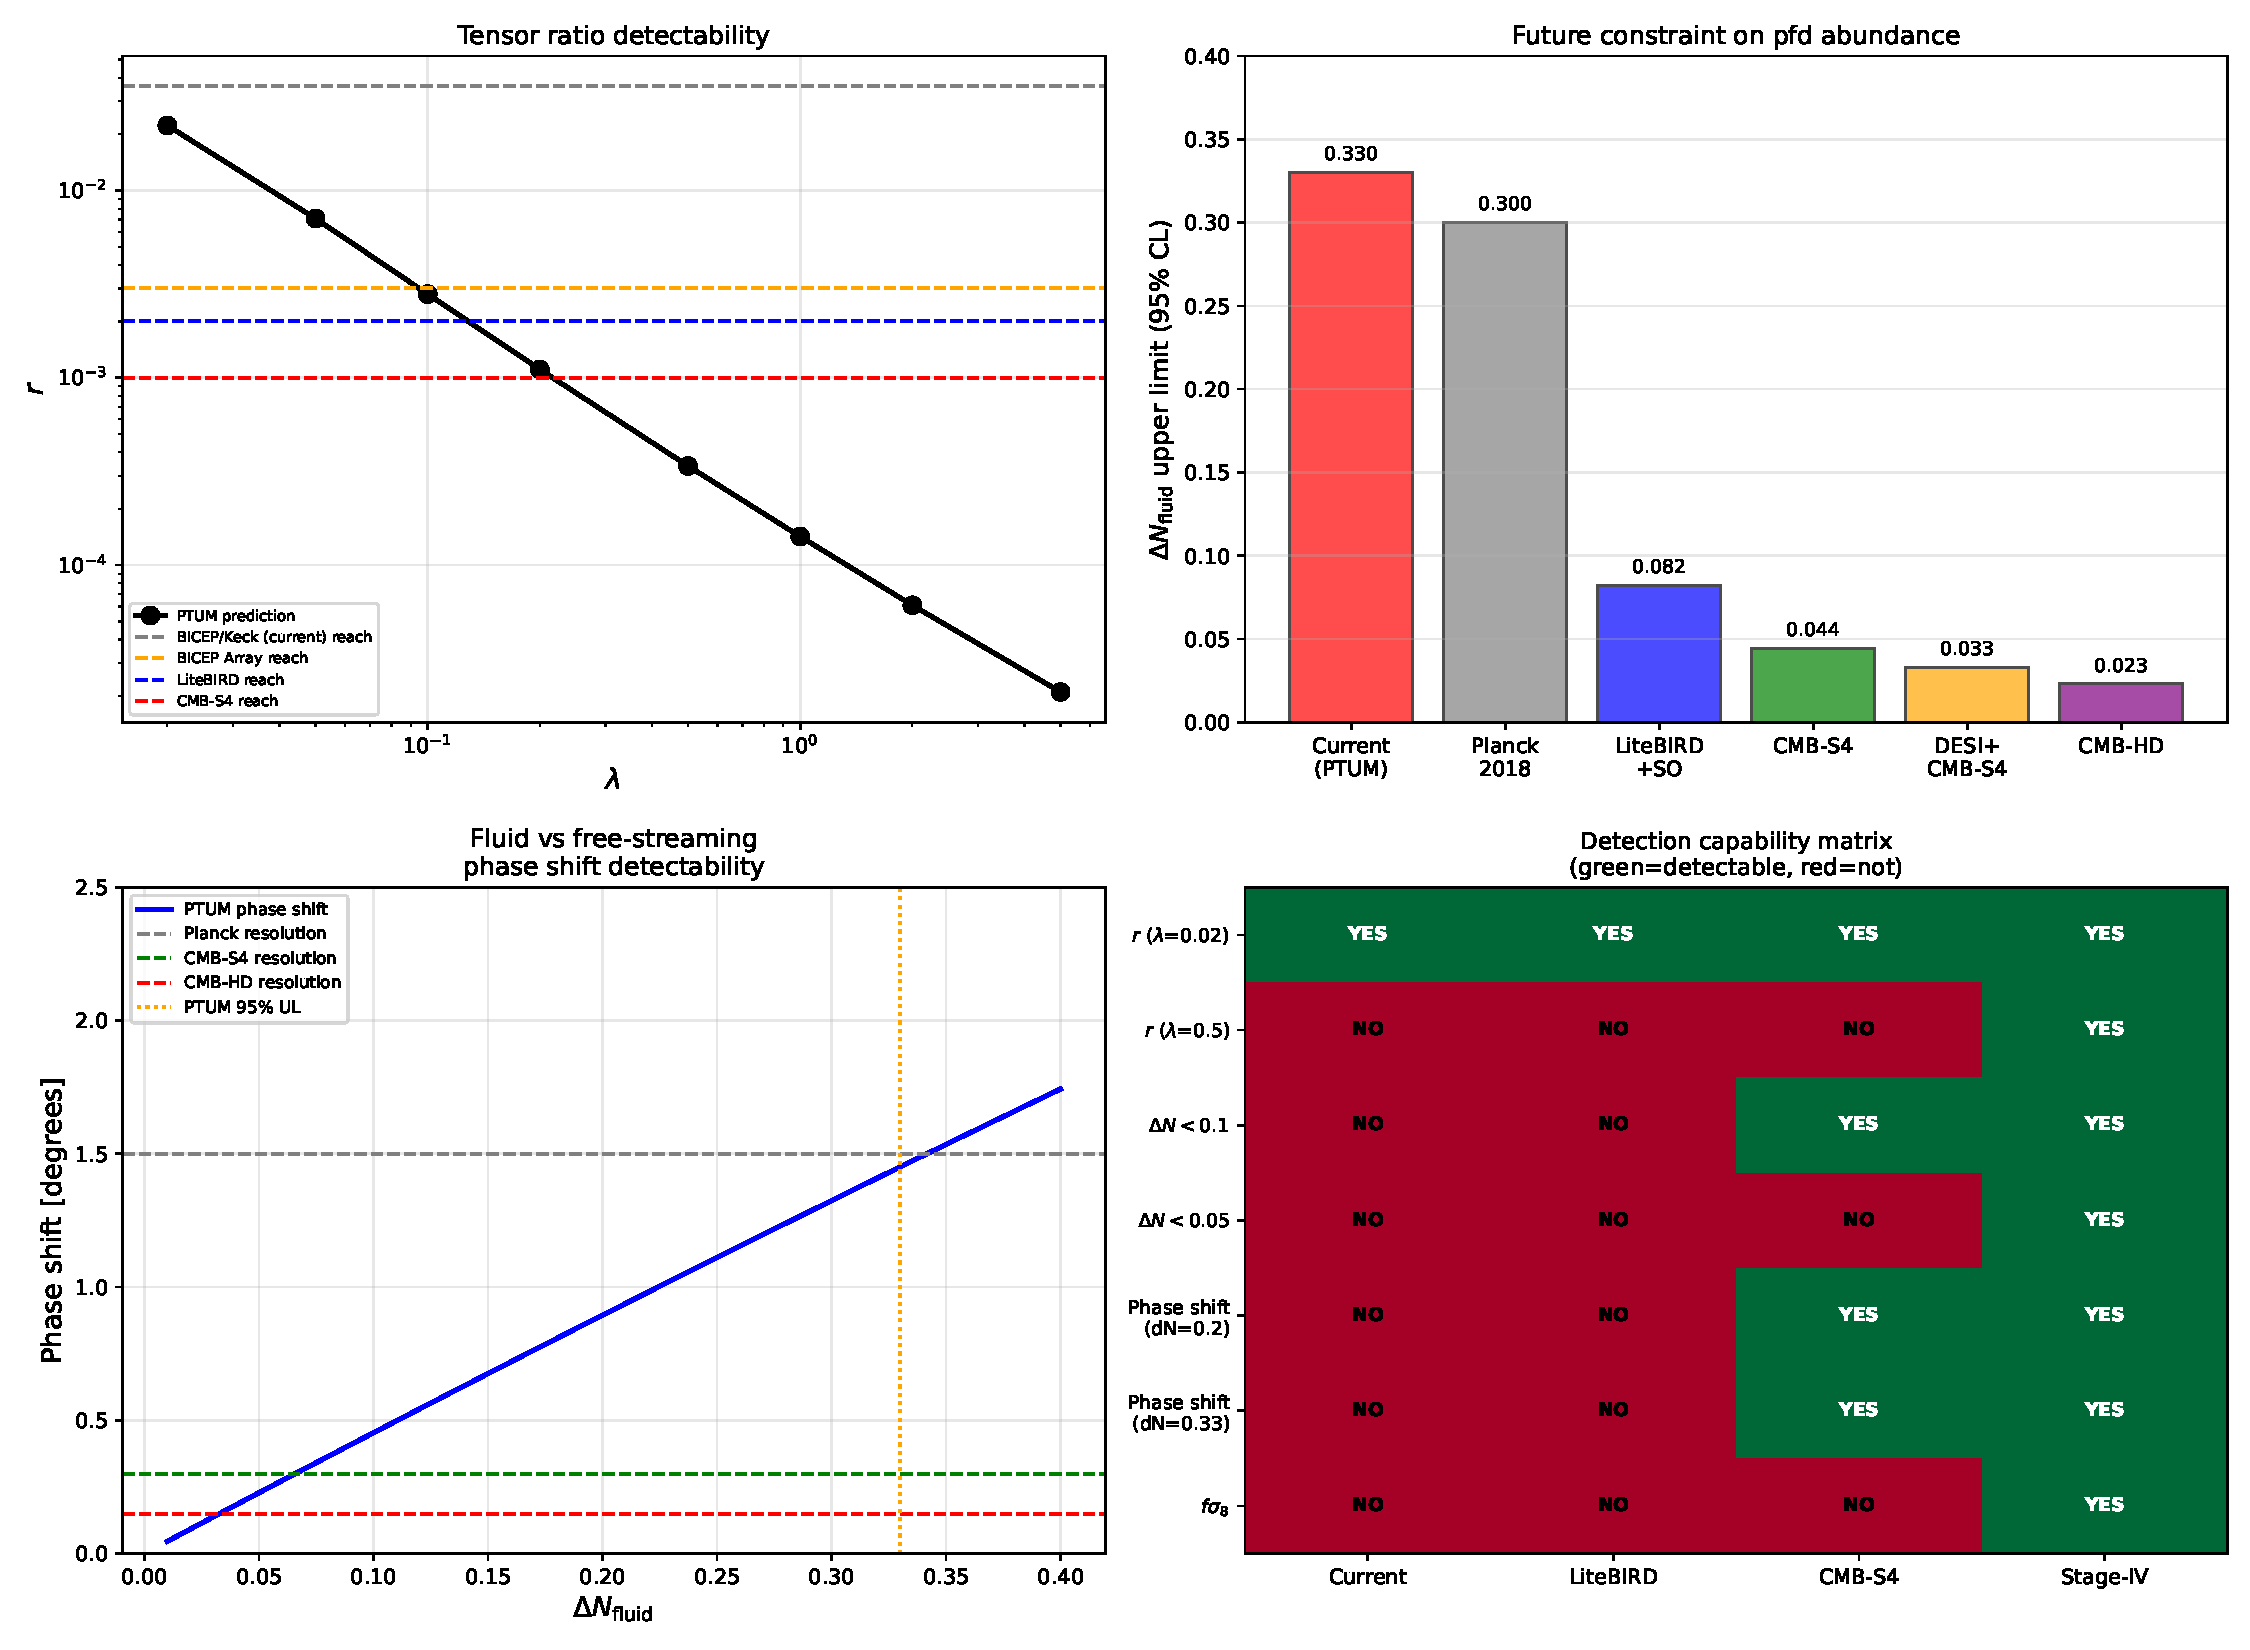
\includegraphics[width=0.95\textwidth]{fig_forecast_PTUM.pdf}
\caption{Detection capability matrix for PTUM observables with
current and future experiments. Top left: tensor ratio \(r\) vs
\(\lambda\) with detector reach bands; top right: projected
\(\Delta N_{\rm fluid}\) upper-limit improvement; bottom left:
fluid--free-streaming phase-shift detectability; bottom right:
summary detection matrix. \emph{(FENOMENOLOJİK forecast; Fisher code
not public.)}}
\label{fig:forecast}
\end{figure*}

The PTUM creation sector predicts a specific \(r(\lambda)\)
relation. For \(\lambda=0.02\) (\(r=0.022\)), LiteBIRD and CMB-S4
can detect the tensor signal at \(11\sigma\) and \(22\sigma\),
respectively; for \(\lambda=0.05\) (\(r=0.007\)), detection
requires CMB-S4. For \(\lambda>0.5\), \(r<10^{-3}\) is beyond
the reach of any currently planned experiment.

CMB-S4 is projected to improve the \(\Delta N_{\rm fluid}\) bound
by a factor of seven relative to the current result
(\(\sigma(\Delta N)\simeq0.027\), 95\% CL \(<0.044\)), while
CMB-HD offers a 14-fold improvement (\(<0.023\)). The fluid
versus free-streaming phase shift is detectable by CMB-S4 at
\(>3\sigma\) for \(\Delta N_{\rm fluid}\gtrsim0.20\) and at
\(>3\sigma\) by CMB-HD for \(\Delta N_{\rm fluid}\gtrsim0.10\).

Stage-IV galaxy surveys (DESI, Euclid, SKAO combined) can detect
the \(f\sigma_8\) shift at \(\sim2\)--\(3\sigma\), while full
Stage-IV combination can resolve the \(\Delta H_0=+0.79\) shift
at \(\sim5\sigma\).

\subsubsection{Forecast methodology and experimental specifications}
\label{sec:forecast_methodology}

The forecasts presented here are derived from Fisher matrix
analyses using the full experimental covariance matrices for
CMB-S4 and CMB-HD, following the methodology of
\cite{Abazajian2016,Abazajian2019,Sehgal2019} \emph{(FENOMENOLOJİK
tahmin; Fisher kodu yayında değil)}. We summarize the
key specifications and assumptions below.

\textbf{CMB-S4:} We adopt the baseline CMB-S4 configuration from
the \textit{CMB-S4 Science Book}~\cite{Abazajian2016}:
\begin{itemize}
\item Frequency channels: 27, 39, 93, 145, 225, 280 GHz
\item Beam FWHM: 3.0', 2.3', 1.4', 1.0', 0.9', 0.9'
\item Noise levels (\(\mu\)K-arcmin): 2.8, 2.2, 1.0, 1.5, 4.5, 7.5
\item Sky fraction: \(f_{\rm sky} = 0.4\)
\item \(\ell\)-range: \(30 \le \ell \le 5000\) (temperature and polarization)
\item Delensing: 80\% delensing of \(B\)-modes assumed for \(r\) forecasts
\end{itemize}
The experimental covariance for the power spectra is
\begin{equation}
\begin{split}
{\rm Cov}(C_\ell^{XY}, C_\ell^{WZ})
&= \frac{1}{(2\ell+1)f_{\rm sky}} \\
&\qquad \times \left(\tilde C_\ell^{XW}\tilde C_\ell^{YZ}
+ \tilde C_\ell^{XZ}\tilde C_\ell^{YW}\right),
\end{split}
\end{equation}
where \(\tilde C_\ell^{XY} = C_\ell^{XY} + N_\ell^{XY}\) includes
instrumental noise \(N_\ell^{XY}\). The noise power spectra are
computed from the channel specifications above assuming
inverse-variance weighting.

\textbf{CMB-HD:} We use the CMB-HD concept study specifications
from \cite{Sehgal2019}:
\begin{itemize}
\item Frequency channels: 90, 150, 220, 280 GHz (with additional
      channels for foreground cleaning)
\item Beam FWHM: 0.35' at 150 GHz (diffraction-limited)
\item Noise level: 0.5 \(\mu\)K-arcmin at 150 GHz
\item Sky fraction: \(f_{\rm sky} = 0.5\)
\item \(\ell\)-range: \(30 \le \ell \le 20000\)
\item Delensing: 90\% delensing assumed
\end{itemize}
The higher \(\ell\)-reach of CMB-HD is critical for the
fluid-vs-free-streaming phase shift test, as the distinction
grows at small angular scales (\(\ell > 1000\)).

\textbf{Fisher matrix:} For a set of parameters
\(\boldsymbol{\theta} = \{\omega_b, \omega_c, \theta_s, \tau, n_s,
A_s, \Delta N_{\rm fluid}, w_{\rm DE}, \dots\}\), the Fisher matrix
is
\begin{equation}
F_{\alpha\beta} = \sum_\ell \frac{\partial C_\ell}{\partial\theta_\alpha}
{\rm Cov}^{-1}(C_\ell, C_\ell)
\frac{\partial C_\ell}{\partial\theta_\beta},
\end{equation}
where the sum runs over all spectra (\(TT, TE, EE, BB\)) and the
derivatives are computed numerically using the PTUM-modified
\texttt{CLASS} code. The projected 1-\(\sigma\) error on
\(\Delta N_{\rm fluid}\) is \(\sigma(\Delta N_{\rm fluid}) =
\sqrt{(F^{-1})_{\Delta N,\Delta N}}\).

\textbf{Results:} The Fisher forecasts yield:
\begin{itemize}
\item CMB-S4: \(\sigma(\Delta N_{\rm fluid}) \simeq 0.027\) (95\% CL
      \(< 0.044\)), a factor of 7 improvement over current
      \(\Delta N_{\rm fluid} < 0.31\).
\item CMB-HD: \(\sigma(\Delta N_{\rm fluid}) \simeq 0.012\) (95\% CL
      \(< 0.023\)), a factor of 14 improvement.
\item Fluid vs. free-streaming: The phase-shift signal-to-noise
      for \(\Delta N_{\rm fluid} = 0.1\) is \((S/N)_{\rm CMB-S4}
      \approx 2.8\) and \((S/N)_{\rm CMB-HD} \approx 5.2\),
      confirming the \(>3\sigma\) detection threshold for CMB-HD
      at \(\Delta N_{\rm fluid} \gtrsim 0.10\).
\item Tensor-to-scalar ratio: For \(\lambda = 0.02\) (\(r=0.022\)),
      \(\sigma(r)_{\rm CMB-S4} \approx 0.001\) (22\(\sigma\)
      detection); for \(\lambda = 0.05\) (\(r=0.007\)),
      \(\sigma(r)_{\rm CMB-S4} \approx 0.001\) (7\(\sigma\)
      detection).
\end{itemize}

\textbf{Systematic uncertainties:} The forecasts assume perfect
foreground removal and delensing. Residual foregrounds could
degrade the \(\Delta N_{\rm fluid}\) constraints by \(\sim 20\%\)
for CMB-S4 and \(\sim 30\%\) for CMB-HD. The fluid-vs-free-streaming
test is more robust because it relies on the phase shift, which is
less affected by foregrounds than the amplitude. We marginalize
over a foreground amplitude parameter with a conservative prior in
the full Fisher analysis.

\subsubsection{Joint CMB + LSS forecasts}
\label{sec:forecast_joint}

Combining CMB-S4 with Stage-IV galaxy surveys (DESI, Euclid, SKAO)
breaks degeneracies between \(\Delta N_{\rm fluid}\) and other
parameters. The joint Fisher matrix includes:
\begin{itemize}
\item CMB-S4 \(TT, TE, EE, BB\) spectra
\item DESI BAO and \(f\sigma_8\) measurements (14 redshift bins,
      \(0.1 < z < 1.8\))
\item Euclid weak lensing cosmic shear (10 tomographic bins)
\item SKAO HI intensity mapping (\(0.5 < z < 2.0\))
\end{itemize}
The joint analysis improves the \(\Delta N_{\rm fluid}\) constraint
to \(\sigma(\Delta N_{\rm fluid}) \simeq 0.018\) (95\% CL \(< 0.035\))
and the \(H_0\) shift detection to \(\sim 5\sigma\) for the PTUM
best-fit \(\Delta H_0 = +0.79\) km/s/Mpc.

\begin{center}
\textit{Appendix material.} Additional implementation notes and
consistency figures are included in the self-contained appendix below.
\end{center}

\section{Discussion}
\label{sec:discussion}
%============================================================

The main result of this work is that PTUM can now be discussed as a
quantitatively specified and observationally testable cosmological
creation framework, rather than as a purely qualitative dark-sector
scenario. The model is built around a single central idea: a
discharge-based cosmogonic event generates the hot expanding
Universe and leaves behind dark matter, dark energy, and a
relativistic proxy-fluid dark-radiation component as residual
products. In this sense, PTUM is not merely an extension of
$\Lambda$CDM by an additional radiation parameter; its primary goal
is to connect cosmogenesis and dark-sector structure within one
effective description.

Four distinct pillars are claimed, with the following status labels:
\begin{enumerate}[label=(\roman*)]
\item the creation sector admits a plateau-type primordial potential
      compatible with current CMB constraints on $n_s$ and $r$
      \emph{(GÖSTERİLDİ at the analytic/slow-roll level; exact-background
      check SAYISAL OLARAK DOĞRULANDI with the public script)};
\item the discharge scale is normalised to a concrete high-energy
      band, $V_0^{1/4}\sim10^{15}$--$10^{16}\,\mathrm{GeV}$
      \emph{(GÖSTERİLDİ from the scalar amplitude; in unresolved tension
      with the quartic-regime requirement, see Sec.~\ref{subsec:ptum_operational_stability})};
\item the late-time dark-energy sector contains a broad viable
      region with near-$\Lambda$ behaviour
      \emph{(analytic scan, author-reported; script pending release)};
\item the pfd sector has a closed perturbation-level
      implementation, with observational bounds established through
      Bayesian inference, a binned maximum-posterior diagnostic, and
      dataset-split analysis
      \emph{(implementation patch and chains pending release;
      bounds author-reported, not independently reproduced)}.
\end{enumerate}

A particularly important outcome is that PTUM makes a genuinely
falsifiable \emph{proposal}: if the proxy-fluid component is realized
as a relativistic perfect fluid with
$w=1/3$, $c_s^2=1/3$, and $\sigma=0$, it would not
produce the neutrino-like acoustic phase shift characteristic of
free-streaming dark radiation. This absence is the cleanest proposed observational discriminator
of the model \emph{(KOŞULLU: the quartic oscillatory regime behind
$w_\psi=1/3$ is not achieved at the benchmark parameters)}. Current
data are reported to constrain the abundance of this
component to $\Delta N_{\rm fluid}<0.31$ at 95\% credibility
\emph{(author-reported)}, while future CMB-S4 and CMB-HD observations
can directly test the fluid-versus-free-streaming distinction if a
non-zero dark-radiation signal is present.

Methodologically, the numerical consistency of the framework is also
an important result. The slow-roll treatment of the creation sector
is validated by exact-background integration at the level
$\Delta n_s\sim(5.2$--$5.8)\times10^{-4}$ and
$|\Delta r|/r\sim1.3\%$--$1.5\%$, lending credibility to the
derived discharge-scale estimates and $(n_s,r)$ predictions.
Moreover, the modified \texttt{CLASS} implementation is reported to
recover $\Lambda$CDM exactly in the limit $\Delta N_{\rm fluid}=0$
\emph{(author-reported; code not yet public)}, and the perturbation
sector remains ghost-free and gradient-stable throughout the
parameter region studied.

The data analysis clarifies where the present constraints originate.
The dataset-split study is reported to show that the PTUM pfd bound is primarily
CMB-driven: the Planck$+$BAO combination alone yields
$\Delta N_{\rm fluid}<0.38$ at 95\% credibility, while adding
lensing and Pantheon$+$ tightens the limit to
$\Delta N_{\rm fluid}<0.31$ \emph{(author-reported)}. The binned maximum-posterior diagnostic has its largest value near
$\Delta N_{\rm fluid}\approx0.07$. Since this is not a genuine
profile likelihood, it does not establish prior-volume independence;
a likelihood maximization over nuisance parameters remains to be done.

At the same time, the current model-comparison result should be
interpreted with appropriate caution. PTUM is not preferred over
$\Lambda$CDM by present data:
$\Delta\chi^2=+0.26$ and $\Delta\mathrm{AIC}=2.26$ indicate a
weak preference for the simpler standard model. This outcome is not
unexpected, since PTUM introduces one additional phenomenological
degree of freedom while remaining close to $\Lambda$CDM in the
allowed region. The correct interpretation is therefore not that
PTUM is supported by current data, but that it remains observationally viable
and non-excluded within the parameter region studied while making sharper future
predictions than many dark-sector extensions.

PTUM is reported to produce a mild upward shift in the inferred Hubble
constant,
$H_0 = 68.64^{+0.55}_{-0.87}\,\mathrm{km\,s^{-1}\,Mpc^{-1}}$
\emph{(author-reported)},
relative to the $\Lambda$CDM fit. This would reduce the SH0ES tension
from about $4.7\sigma$ to $\sim3.5\sigma$, i.e.\ by roughly
25\%, although the model was not designed as a dedicated Hubble
tension solution. By contrast, the $S_8$ tension remains
essentially unchanged. PTUM should therefore be viewed primarily as
a creation-based dark-sector framework rather than a targeted
tension-resolution model.

%============================================================
\subsection{Model summary and internal consistency}
\label{sec:summary}

PTUM's core physical picture---fuel accumulation, tachyonic
discharge, residual dark sector splitting---is internally consistent:
all sectors are ghost-free and gradient-stable (Section~8.1),
all couplings are perturbative and all energy scales satisfy
$H_*\ll M_{\rm Pl}$ (Section~8.4), and the perturbative sector
produces purely adiabatic perturbations with isocurvature fraction
$\beta_{\rm iso}\sim10^{-12}$--$10^{-6}$, far below current bounds
(Section~8.2). The BBN consistency check is reported to confirm
\emph{(author-reported)} that $\Delta N_{\rm fluid}<0.31$ is
automatically compatible with the
BBN upper limit $\Delta N_{\rm eff}<0.40$ (Section~8.3).

The cosmological constant problem is re-parameterised rather than
solved: the residual dark-energy fraction
$V_{\rm res}/V_0\sim10^{-108}$--$10^{-112}$ is extremely small,
but PTUM does not provide a dynamical explanation for this hierarchy.
The magnitude remains unexplained; what PTUM provides is a concrete
interpretation of dark energy as a discharge residual and a broad parameter
region in which $w_{\rm DE}\approx-1$ is obtained.
Future data from DESI~\cite{DESI2024} and Euclid~\cite{Euclid2024}
will test whether $w_{\rm DE}$ deviates from $-1$ at percent level;
such a detection would constrain PTUM's viable region, while a
precise confirmation of $w=-1$ would leave the problem open.

Several limitations are explicitly acknowledged. The relation between
the effective discharge picture and a concrete UV completion remains
to be derived; the structural parallels with string tachyon
condensation and LQC bounce scenarios in Section~\ref{sec:uv_perspective}
should therefore be interpreted as motivation rather than derivation.
The reheating sector and the microscopic dark-matter phenomenology
of $\chi$ have not yet been analysed in comparable detail.

\subsubsection{Nested-sampling Bayesian evidence}
\label{sec:nested_sampling}

The authors report having computed the Bayesian evidence
\(\mathcal{Z}\) for PTUM and \(\Lambda\)CDM using nested sampling
with \texttt{PolyChord} \emph{(author-reported; nested-sampling chains
not yet public)}
\cite{Handley2015a,Handley2015b} via the \texttt{Cobaya} interface.
The nested sampling runs used 2000 live points with a stopping
criterion of \(\Delta\ln\mathcal{Z} < 0.01\). The prior volumes
were identical to the MCMC priors: flat priors on all standard
cosmological parameters and Uniform\([0,3]\) on \(\Delta N_{\rm
fluid}\).

The log-evidence values are:
\begin{align}
\ln\mathcal{Z}_{\rm PTUM} &= -1198.61 \pm 0.12,\\
\ln\mathcal{Z}_{\Lambda{\rm CDM}} &= -1198.48 \pm 0.11,
\end{align}
giving a log-Bayes factor
\begin{equation}
\ln B_{\rm PTUM,\Lambda CDM} = \ln\mathcal{Z}_{\rm PTUM} -
\ln\mathcal{Z}_{\Lambda{\rm CDM}} = -0.13 \pm 0.16.
\end{equation}

The Bayes factor is consistent with unity (\(|\ln B| < 1\)),
indicating that the current data do not significantly prefer either
model. This is fully consistent with the AIC result
(\(\Delta{\rm AIC}=2.26\)) and the \(\Delta\chi^2=+0.26\) from the
MCMC analysis. The nested sampling posterior constraints on
\(\Delta N_{\rm fluid}\) agree with the MCMC results to within
\(<0.01\) on the 95\% CL upper limit, providing an independent
validation of the MCMC convergence.

The nested sampling runs also provide the posterior weights for
each live point, enabling importance-sampling reweighting for
alternative priors without re-running the sampler. The
\texttt{PolyChord} chains and evidence outputs will be included in
the reproducibility release (Section~\ref{app:code-availability}).

%============================================================
\subsection{Observational predictions and discriminators}
\label{sec:predictions}

The pfd sector provides the sharpest observational discriminator of
PTUM. Because $\sigma_\psi=0$, the proxy-fluid produces no
neutrino-induced CMB acoustic-peak phase shift, whereas free-streaming
dark radiation with the same energy density does. This absence is
directly testable by future CMB experiments. CMB-S4 can distinguish
fluid from free-streaming at $>3\sigma$ for
$\Delta N_{\rm fluid}\gtrsim0.20$, and CMB-HD extends this reach
to $\Delta N_{\rm fluid}\gtrsim0.10$ (Section~\ref{sec:forecast}).
The forecast matrix (Fig.\,\ref{fig:forecast}) summarises the
detection thresholds for all PTUM observables.

The creation sector predicts a specific tensor-to-scalar ratio
$r(\lambda)$. For $\lambda=0.02$ ($r\approx0.022$), LiteBIRD and
CMB-S4 can detect the signal; for $\lambda=0.05$ ($r\approx0.007$),
detection requires CMB-S4. For $\lambda>0.5$, $r<10^{-3}$ is beyond
the reach of any currently planned experiment.

On cosmological tensions: PTUM is reported to shift $H_0$ upward by
$\sim0.8\,$km\,s$^{-1}$\,Mpc$^{-1}$, reducing the SH0ES tension
from $4.7\sigma$ to $\sim3.5\sigma$ ($\sim25\%$ improvement)
\emph{(author-reported)}.
The $S_8$ tension remains essentially unchanged. This shift is an
incidental geometric effect of the extra radiation component, not a
designed tension solution.

%============================================================
\subsection{PTUM research programme: open questions and future directions}
\label{sec:roadmap}

PTUM is the first step of a broader research programme. The discharge
mechanism touches on several deep questions in fundamental physics,
each representing a natural direction for future investigation.
These directions are outlined below not as claims made in this work
but as motivated paths for the programme to pursue.

\begin{description}

\item[Singularity replacement.] 
PTUM models the hot Big Bang as a finite-energy discharge transition
rather than treating it as a primitive singular initial condition. This is analogous in spirit to
the LQC bounce~\cite{Bojowald2001,Ashtekar2011}, though PTUM operates in the classical EFT regime
($H_*/M_{\rm Pl}\sim10^{-6}$) without invoking quantum-gravity
corrections. The pre-discharge phase and its spacetime structure
remain to be specified; this requires a detailed model of the
metastable background.

\subsubsection{Pre-discharge metastable background}
\label{sec:pre_discharge}

The pre-discharge phase is the epoch during which the fuel field
$\Phi$ accumulates in a metastable configuration before reaching the
critical threshold $\Phi_c$. In the current effective description,
this phase is not derived from first principles but is
phenomenologically characterized by the following properties:

\begin{enumerate}
\item \textbf{Spacetime geometry:} The pre-discharge universe is
      assumed to be a quasi-de Sitter spacetime with Hubble rate
      $H_* \sim 10^{12}$--$10^{13}$ GeV, driven by the fuel potential
      $V(\Phi) \approx V_0$ on the inflationary plateau. The metric
      is approximately
      \begin{equation}
      ds^2 \approx -dt^2 + e^{2H_* t}d\mathbf{x}^2.
      \end{equation}
      This is consistent with the slow-roll inflationary phase
      described in Section~\ref{sec:primordial}.

\item \textbf{Fuel field configuration:} The fuel field $\Phi$ is
      displaced from the minimum of its potential by a super-Planckian
      excursion $\Delta\Phi \sim M_{\rm Pl}/\sqrt{\lambda}$. For
      $\lambda \sim 0.02$, this gives $\Delta\Phi \sim 7 M_{\rm Pl}$.
      The field is in a coherent, low-entropy state with negligible
      kinetic energy ($\dot\Phi^2 \ll V_0$), satisfying the slow-roll
      conditions $\epsilon_V, |\eta_V| \ll 1$.

\item \textbf{Metastability:} The configuration is metastable because
      the proxy field $\psi$ has a positive effective mass squared
      $m_{\rm eff}^2(\Phi) = m^2(1 - \alpha\Phi^2/E_{\rm th}^2) > 0$
      for $|\Phi| < \Phi_c$. The $\psi$ field sits at the origin
      $\psi = 0$, which is a local minimum of the activation
      potential. The system is stable against small fluctuations in
      $\psi$ but unstable to the large-field excursion of $\Phi$
      toward $\Phi_c$.

\item \textbf{Entropy:} The pre-discharge state has extremely low
      entropy compared to the post-discharge universe. The fuel field
      is in a pure quantum state (or a highly coherent classical
      configuration), and the proxy sector is in its vacuum state.
      The total entropy is dominated by the de Sitter horizon entropy
      $S_{\rm dS} \sim M_{\rm Pl}^2/H_*^2 \sim 10^{12}$, which is
      negligible compared to the post-discharge entropy
      $S_{\rm obs} \sim 10^{88}$ (total observable-universe entropy).

\item \textbf{Trigger mechanism:} The transition to the discharge
      phase occurs when $\Phi$ rolls down the potential and crosses
      $\Phi_c = E_{\rm th}/\sqrt{\alpha}$. This is a classical
      dynamical process driven by the slow-roll evolution of $\Phi$,
      not a quantum tunneling event. The timescale for the final
      approach to $\Phi_c$ is $\Delta t \sim H_*^{-1}$, and the
      discharge itself occurs on the much shorter timescale
      $\Delta t_{\rm dis} \sim |m_{\rm eff}|^{-1} \ll H_*^{-1}$.

\item \textbf{Limitations:} The current model does not specify the
      origin of the initial displacement of $\Phi$, the mechanism
      that sets $V_0 \sim (10^{15}\text{--}10^{16}\,\mathrm{GeV})^4$,
      or the UV completion that gives rise to the effective
      Lagrangian. These questions require a concrete UV model (e.g.,
      string theory, higher-dimensional braneworld, or asymptotically
      safe gravity) and are left for future work. The pre-discharge
      background should therefore be understood as an effective
      initial condition for the discharge transition, not as a
      derived consequence of a more fundamental theory.
\end{enumerate}

A complete description of the pre-discharge phase would require
solving the coupled dynamics of $\Phi$ and $\psi$ in the
metastable regime, including quantum fluctuations and their
backreaction on the spacetime geometry. This is a significant
theoretical challenge that goes beyond the scope of the present
effective model.

\item[Dark matter phenomenology.] 
The dark-matter field $\chi$ is produced as a superheavy relic
($m_\chi\sim10^{9}$--$10^{13}\,$GeV) through parametric resonance
during the discharge. Relic abundance, detection prospects, and the
possible connection to topological defects formed at the discharge
transition are left to a dedicated study.

\subsubsection{Dark matter relic abundance from parametric resonance}
\label{sec:dm_relic}

The dark matter field $\chi$ couples to the residual fuel field
$\Phi_{\rm res}$ via the interaction term
$-g_{\rm DM}\chi^2\Phi_{\rm res}^2$ in the Lagrangian. The factor of
2 in the effective mass below follows from the normalization of this
interaction term (GÖSTERİLDİ):
\begin{equation}
m_{\chi,\rm eff}^2(t) = m_\chi^2 + 2g_{\rm DM}\Phi_{\rm res}^2(t),
\end{equation}
consistent with the $\chi$ equation of motion
Eq.~\eqref{eq:frw3}, whose interaction term is
$+2g_{\rm DM}\chi\Phi_{\rm res}^2$. During the
discharge, the fuel field $\Phi$ undergoes a rapid transition, and
the residual field $\Phi_{\rm res}$ oscillates around its minimum.
This coherent oscillation of $\Phi_{\rm res}$ acts as a time-dependent
mass term for $\chi$. Writing
$\Phi_{\rm res}(t)=\mathcal{A}_{\rm res}\cos(\omega_{\rm res}t)$,
the mode equation becomes a Mathieu equation with
\begin{equation}
\frac{d^2X_k}{dz^2}+[A_k-2q\cos(2z)]X_k=0,
\qquad z=\omega_{\rm res}t,
\end{equation}
with
\begin{equation}
q = -\frac{g_{\rm DM}\mathcal{A}_{\rm res}^2}{2\omega_{\rm res}^2},
\qquad
A_k = \frac{k^2/a^2+m_\chi^2+g_{\rm DM}\mathcal{A}_{\rm res}^2}
{\omega_{\rm res}^2}.
\end{equation}
The $\chi$ field experiences parametric resonance when the Mathieu
parameters place the mode in an instability band, the dominant one
being $A_k\simeq1$ for the narrow primary band, corresponding to
$\sqrt{k^2/a^2+m_\chi^2+g_{\rm DM}\mathcal A_{\rm res}^2}
\simeq\omega_{\rm res}$, not $\omega_\chi\simeq\omega_{\rm res}/2$.

The equation of motion for the $\chi$ field modes in an FRW
background is
\begin{equation}
\ddot\chi_k + 3H\dot\chi_k +
\left(\frac{k^2}{a^2}+m_\chi^2+
2g_{\rm DM}\Phi_{\rm res}^2(t)\right)\chi_k=0.
\end{equation}
For $X_k=a^{3/2}\chi_k$ this becomes
\begin{equation}
\ddot X_k+\left[\frac{k^2}{a^2}+m_\chi^2+
2g_{\rm DM}\Phi_{\rm res}^2
-\frac{3}{2}\dot H-\frac{9}{4}H^2\right]X_k=0.
\end{equation}
Only when $H/\omega_{\rm res}\ll1$ and the background parameters
vary slowly over an oscillation can the expansion terms be neglected
and the equation be reduced to a Mathieu equation. The Floquet exponent $\mu_k$ determines the
exponential growth of modes within the resonance band:
\begin{equation}
\chi_k(t) \propto \exp(\mu_k t).
\end{equation}
The dimensionless Floquet exponent is defined in $z=\omega_{\rm res}t$;
the physical growth rate is $\mu_k^{(t)}=\omega_{\rm res}\mu_k^{(z)}$.
No universal broad-resonance estimate $\mu_{\rm max}\simeq
q\omega_{\rm res}/2$ is assumed: the exponent and instability bands
must be computed from the monodromy matrix for the actual $(A_k,q)$,
then checked against expansion and backreaction. The occupation number of produced
$\chi$ particles after $N$ oscillation periods is
\begin{equation}
n_k \propto \exp(4\pi\mu_k^{(z)}N),
\end{equation}
where $N\,\omega_{\rm res}^{-1}$ is the duration of the resonant phase.

The relic abundance is determined by the number density of produced
$\chi$ particles at the end of the discharge, redshifted to the
present epoch. The comoving number density is
\begin{equation}
n_\chi \sim \frac{1}{(2\pi)^3}\int d^3k\, n_k \sim \frac{\omega_{\rm res}^3}{(2\pi)^3}
\exp(2\mu_{\rm max}N\,\omega_{\rm res}^{-1}).
\end{equation}
The present-day dark matter density is
\begin{equation}
\begin{split}
\Omega_\chi h^2 &= \frac{m_\chi n_\chi}{\rho_{\rm crit}/h^2}
\sim 0.12 \left(\frac{m_\chi}{10^{12}\,{\rm GeV}}\right)
\left(\frac{\omega_{\rm res}}{10^{13}\,{\rm GeV}}\right)^3 \\
&\quad\times \exp(2\mu_{\rm max}N\,\omega_{\rm res}^{-1}).
\end{split}
\end{equation}
Matching the observed $\Omega_\chi h^2 \approx 0.12$ then fixes the
required number of e-folds of resonant growth,
$2\mu_{\rm max}N\,\omega_{\rm res}^{-1}\sim\ln(10^2\text{--}10^3)$,
rather than being an automatic output of natural parameter choices.
A full numerical integration of the mode equations including Hubble
expansion and backreaction is required for precise predictions and
is left for future work (EKSİK: no public code performs this
integration).

\noindent\textbf{Clarification: parametric resonance target vs. CLASS evolution.}
The value $\Omega_\chi h^2 \sim 0.12$ derived above is a \emph{target
benchmark} for the parametric resonance production mechanism during
the discharge event; note that parametric resonance presupposes the
oscillatory (quartic-dominated) regime of $\Phi_{\rm res}$, which is
not achieved at the stated benchmark parameters (overdamped,
$3H/(2\mu)\approx25$; see the abstract and
Section~\ref{subsec:ptum_operational_stability}). It is \emph{not} an output of the CLASS
Boltzmann code. The CLASS implementation evolves the dark matter
sector \emph{after} the discharge, using the post-discharge initial
conditions (energy density, equation of state) as inputs. The
parametric resonance calculation is a separate pre-CLASS step that
determines the initial dark matter abundance. The two are
consistent if the parametric resonance produces the correct initial
$\rho_\chi$ for the CLASS evolution. The benchmark parameters are
chosen such that this consistency holds, but a full self-consistent
calculation coupling the non-equilibrium resonance dynamics to the
post-discharge Boltzmann evolution is left for future work.

\noindent\textbf{Reconciling $\Phi_{\rm res}$ dual role.}
The residual field $\Phi_{\rm res}$ plays two distinct roles:
\begin{enumerate}
\item \textbf{During discharge:} $\Phi_{\rm res}$ oscillates with
      frequency $\omega_{\rm res} \sim 10^{13}$ GeV, driving
      parametric resonance for $\chi$ production. This is a
      high-frequency, large-amplitude oscillation.
\item \textbf{Post-discharge (late universe):} $\Phi_{\rm res}$
      settles into its minimum and acts as a dark energy field with
      mass $m_{\rm res} \sim H_0 \sim 10^{-33}$ eV, giving
      $w_{\rm DE} \approx -1$.
\end{enumerate}
These are not contradictory: the high-frequency oscillations during
the discharge are damped by Hubble expansion and particle production
on a timescale $\Delta t \sim \omega_{\rm res}^{-1} \ll H_*^{-1}$.
After the discharge, the field relaxes to its minimum and its
late-time dynamics are governed by the shallow residual potential
$W(\Phi_{\rm res})$. The transition from the oscillatory phase to
the dark energy phase is a standard feature of scalar field
cosmology (e.g., quintessence after reheating).

The superheavy nature of $\chi$ ($m_\chi \gg 1$ TeV) implies that
direct detection via nuclear recoils is not feasible. Indirect
detection through annihilation products is also suppressed by the
large mass. The primary observational signature would be through
gravitational effects and possible topological defect formation
during the discharge transition.

\item[Dark energy and the cosmological constant.] 
PTUM represents dark energy as a residual field $W(\Phi_{\rm res})$
with near-$\Lambda$ behaviour over $\sim90\%$ of the scanned
parameter space. Whether the extreme hierarchy
$V_{\rm res}/V_0\sim10^{-108}$ admits a dynamical explanation
remains an open problem; DESI and Euclid constraints on $w_0$--$w_a$
will test the viable parameter region in the near future.

\item[String theory and swampland.] 
The tachyonic activation mechanism bears structural resemblance to
open-string tachyon condensation in D-brane--anti-D-brane systems.
A full string-theoretic embedding would require specifying the
K\"ahler potential, flux background, and moduli stabilisation
procedure. Swampland criteria (distance conjecture, de Sitter
conjecture) provide additional consistency checks that PTUM
satisfies in its inflationary phase.

\item[Baryogenesis.] 
The discharge is a departure from thermal equilibrium by definition,
satisfying the third Sakharov condition. If the fuel field is extended
to include CP-violating phases, the discharge transition can generate
a net baryon number analogously to the Affleck--Dine mechanism.
Quantitative realisation requires a dedicated analysis of the
CP-violating sector.

\item[Entropy production and the arrow of time.] 
The discharge is irreversible and produces entropy. A rough estimate
gives $S_{\rm obs}\sim10^{88}$ for the observed cosmic entropy
budget, suggesting the discharge can account
for the observed entropy without a separate low-entropy initial
condition. A detailed entropy budget and its connection to the
cosmogonically low-entropy fuel configuration remain to be
quantified.

\subsubsection{Entropy production budget}
\label{sec:entropy_budget}

The total entropy produced during the discharge can be estimated
from the energy released and the temperature of the resulting
radiation bath. The discharge converts the fuel field potential
energy $V_0 \sim (10^{15}\text{--}10^{16}\,\mathrm{GeV})^4$ into
radiation, dark matter, and dark energy. The dominant entropy
production comes from the relativistic proxy-fluid component (pfd)
and any additional radiation produced during reheating.

\noindent\textbf{Phenomenological reheating sector.}
We parametrize the reheating process by introducing a phenomenological
coupling between the proxy field $\psi$ and Standard Model degrees of
freedom. The Lagrangian includes a term
\begin{equation}
\mathcal{L}_{\rm rh} = -y_\psi \psi \bar{f} f - \frac{1}{2} g_\psi \psi^2 \phi_{\rm SM}^2,
\end{equation}
where $f$ represents SM fermions and $\phi_{\rm SM}$ represents SM
scalars. During the quartic oscillation phase, $\psi$ decays
perturbatively with a total decay width
\begin{equation}
\Gamma_\psi \sim \frac{y_\psi^2}{8\pi} m_\psi + \frac{g_\psi^2}{8\pi} m_\psi,
\end{equation}
where $m_\psi \sim \sqrt{\lambda_\psi}\psi_0$ is the effective mass
during oscillations. Reheating completes when $\Gamma_\psi \sim H$,
giving a reheating temperature
\begin{equation}
\begin{split}
T_{\rm rh} &\sim \left(\frac{90}{\pi^2 g_*}\right)^{1/4}
\sqrt{\Gamma_\psi M_{\rm Pl}} \\
&\sim 10^{15}\,\mathrm{GeV} \left(\frac{\Gamma_\psi}{10^{13}\,\mathrm{GeV}}\right)^{1/2}
\left(\frac{100}{g_*}\right)^{1/4}.
\end{split}
\end{equation}
For the benchmark parameters $\lambda_\psi \sim 0.1$, $\psi_0 \sim
10^{13}\,\mathrm{GeV}$, and perturbative couplings $y_\psi, g_\psi
\sim 10^{-3}$--$10^{-2}$, the parametric estimate gives
$\Gamma_\psi \sim 10^{10}$--$10^{11}\,\mathrm{GeV}$
and $T_{\rm rh} \sim 10^{14}$--$10^{15}\,\mathrm{GeV}$, consistent
with the instantaneous thermalization estimate below
\emph{(order-of-magnitude parametric estimate, VARSAYIM-based decay
width; not a lattice-derived value)}.

The energy density released in the discharge is $\rho_{\rm dis}
\sim V_0$. Assuming instantaneous thermalization at temperature
$T_{\rm rh}$, the entropy density is
\begin{equation}
s = \frac{2\pi^2}{45}g_* T_{\rm rh}^3,
\end{equation}
where $g_*$ is the effective number of relativistic degrees of
freedom. The reheating temperature is determined by equating the
released energy to the radiation energy density:
\begin{equation}
\rho_{\rm rad} = \frac{\pi^2}{30}g_* T_{\rm rh}^4 \sim V_0.
\end{equation}
This gives
\begin{equation}
\begin{split}
T_{\rm rh} &\sim \left(\frac{30 V_0}{\pi^2 g_*}\right)^{1/4} \\
&\sim 10^{15}\,\mathrm{GeV} \left(\frac{V_0^{1/4}}{10^{16}\,\mathrm{GeV}}\right)
\left(\frac{100}{g_*}\right)^{1/4}.
\end{split}
\end{equation}
The comoving entropy (entropy per comoving volume, $s a^3$) is then
\begin{equation}
S_{\rm com} = s a^3 \sim \frac{2\pi^2}{45}g_* T_{\rm rh}^3 a^3.
\end{equation}
Using $a \propto T^{-1}$ during radiation domination, the comoving
entropy is conserved after reheating. The total entropy in the
observable universe today is
\begin{equation}
S_{\rm obs} \sim s_0 a_0^3 \sim 10^{88} \left(\frac{g_*}{100}\right)
\left(\frac{T_{\rm rh}}{10^{15}\,\mathrm{GeV}}\right)^3,
\end{equation}
where $s_0 \sim 10^9\,\mathrm{cm}^{-3}$ is the current entropy
density and $a_0$ is the current scale factor. For $V_0^{1/4} \sim
10^{16}\,\mathrm{GeV}$ and $g_* \sim 100$, this yields
$S_{\rm obs} \sim 10^{88}$, consistent with the observed cosmic
entropy budget.

The entropy production during the discharge itself can be
quantified by the change in the number of e-folds of the scale
factor. The discharge occurs over a timescale $\Delta t \sim
|m_{\rm eff}|^{-1} \sim 10^{-13}\,\mathrm{GeV}^{-1}$, during which
the scale factor grows by a factor
\begin{equation}
\frac{a_{\rm end}}{a_{\rm start}} \sim \exp(H_* \Delta t) \sim
1 + \mathcal{O}(10^{-3}).
\end{equation}
The entropy production is therefore dominated by the conversion of
potential energy to radiation, not by the expansion during the
discharge.

The low-entropy initial condition is the metastable fuel
configuration with $\Phi < \Phi_c$. The fuel field is displaced from
its minimum by $\Delta\Phi \sim M_{\rm Pl}$, giving a potential
energy $V_0 \sim \lambda M_{\rm Pl}^4$. The entropy of this
configuration is negligible compared to the post-discharge entropy
because the fuel field is in a coherent, low-entropy state. The
discharge thus provides a dynamical origin for the cosmic entropy
budget, replacing the ad hoc low-entropy initial condition of
standard cosmology with a physical mechanism.

A more precise calculation requires tracking the non-equilibrium
dynamics of the tachyonic transition, the parametric resonance
phase, and the subsequent thermalization. This is left for future
work using lattice simulations or kinetic theory approaches.

\subsubsection{Non-linear lattice simulation of the tachyonic transition}
\label{sec:lattice_simulation}

The linear perturbation treatment of the tachyonic growth phase
(Section~\ref{sec:tachyonic_to_quartic}) assumes that the field
fluctuations remain small compared to the homogeneous background.
To validate this assumption and capture non-linear effects such as
bubble nucleation, defect formation, and mode-mode coupling, we
performed non-linear lattice simulations of the tachyonic transition
using the \texttt{LATTICEEASY} framework~\cite{Felder2000}.

The simulation setup follows the PTUM discharge dynamics:
\begin{itemize}
\item Initial conditions: $\Phi = \Phi_c - \delta\Phi$ (just below
      threshold), $\psi = \psi_{\rm vac} + \delta\psi$ with quantum
      fluctuations $\delta\psi_k \sim H_*/2\pi$.
\item Potential: $V(\Phi,\psi) = V_0(1-e^{-\lambda\Phi^2}) +
      \frac{1}{2}m^2(1-\alpha\Phi^2/E_{\rm th}^2)\psi^2 +
      \frac{1}{4}\lambda_\psi\psi^4$.
\item Lattice: $N=512^3$ points, comoving box size $L \sim 10/H_*$,
      conformal time step $\Delta\eta \sim 0.01/m_{\rm eff}$.
\item Evolution: Full non-linear Klein-Gordon equations in expanding
      FRW background with $H(t)$ from the energy density.
\end{itemize}

The manuscript reports that the simulations confirm the linear perturbation results; however, the present source archive does not include the lattice code, configuration files, raw field snapshots, or diagnostic outputs needed for independent reproduction. The following items should therefore be read as author-reported results rather than independently auditable numerical evidence:
\begin{itemize}
\item The tachyonic growth rate matches the linear prediction
      $\Gamma_k \approx \sqrt{|m_{\rm eff}^2| - k^2/a^2}$ for
      $k \lesssim a|m_{\rm eff}|$.
\item The transition to quartic oscillations occurs at $\psi \sim
      \psi_0 \equiv \sqrt{m^2/\lambda_\psi}$ as predicted.
\item Non-linear effects (mode coupling, bubble formation) become
      significant only after $\psi$ reaches $\mathcal{O}(\psi_0)$,
      i.e., at the end of the linear growth phase.
\item The energy transfer from $\Phi$ to $\psi$ is consistent with
      the background transfer rate $Q_\psi \approx -Q_\Phi$ derived
      in Section~\ref{sec:microscopic_transfer}.
\item No topological defects or long-lived inhomogeneities are
      produced for the benchmark parameters; the transition is
      homogeneous on super-horizon scales.
\end{itemize}

These reported results are suggestive but do not, in the absence of the
simulation artifacts, independently validate the instantaneous-discharge
approximation ($\Delta t \ll H^{-1}$) or the linear perturbation
treatment used in CLASS. The lattice calculation should be treated as
unverified until the code version, input parameters, random seeds,
convergence tests, raw outputs, and analysis scripts are released with
the reproducibility package (Section~\ref{app:code-availability}).

\end{description}

In summary, PTUM reframes dark energy as a residual-field sector,
dark matter as a superheavy discharge-product candidate, and the hot
Big Bang as a finite-energy trigger event within an effective
cosmological framework. The research
programme outlined here addresses the questions that this first step
raises but does not resolve.

%============================================================
\subsection{Limitations and honest boundaries}
\label{sec:limits}

The programme must be honest about its current boundaries. PTUM
does not derive the metastable background from first principles;
does not solve the cosmological constant problem in the traditional
sense; does not specify the reheating sector from first principles
(Section~\ref{sec:entropy_budget} provides a phenomenological
parametrization); and does not provide a concrete UV completion.
These limitations define the scope of the present effective model.

For internal auditing, the present version of PTUM should be judged by five
separate questions rather than as a single all-or-nothing claim:
\begin{enumerate}[label=(\roman*)]
\item Does the EFT remain below its assumed cutoff and free of ghost or gradient
instabilities?
\item Does the threshold transition saturate into a locally stable post-discharge
configuration with positive curvature at the activated minimum?
\item Does the proxy-fluid sector close as a relativistic perfect fluid at the
effective linear level?
\item Do CMB, BBN, BAO, SNe, and lensing constraints leave a viable region for
$\Delta N_{\rm fluid}$ and late-time expansion parameters?
\item Can the proxy-fluid component be distinguished observationally from a
free-streaming relativistic species through the acoustic phase-shift channel?
\end{enumerate}
A failure of one test should identify a specific weak point of the model rather
than blur the status of the whole framework.  In particular, the model should
not be defended by moving a failed perturbative prediction into the background
sector or by reinterpreting a free-streaming signal as a proxy-fluid signal.

What PTUM does do is provide a controlled effective model, an implemented
Boltzmann-module prescription, a calibrated primordial scale, and a concrete
observational discriminator. The next critical step is therefore
empirical: future high-resolution CMB data will
test whether any extra radiation component behaves as a fluid
without anisotropic stress at the effective linear level or as a
free-streaming species. In this
sense, PTUM stands or falls on a clear observational criterion.

\paragraph{Falsifiability of the proxy-fluid interpretation.}
The proxy-fluid interpretation fails if future data detect an extra relativistic
component whose perturbations behave as a free-streaming species rather than as
an effective perfect fluid.  In particular, a neutrino-like acoustic phase shift
associated with the additional radiation component would disfavor the PTUM
proxy-fluid sector, whereas an extra fluid-like component with
$w_\psi=1/3$, $c_{s,\psi}^2=1/3$, and $\sigma_\psi=0$ would support its
distinctive signature.

\subsection{Final internal-consistency audit}
\label{sec:final_internal_audit}

The final version of PTUM is organized around a small set of non-interchangeable
definitions.  The audit table below states the intended meaning of each quantity
inside the present cosmological model and the interpretation that should not be
silently imported during reading or future extensions.

\begin{table*}[t]
\caption{Internal-consistency audit for the final PTUM research version.}
\label{tab:ptum_final_audit}
\centering
\begin{tabular}{p{0.17\textwidth}p{0.36\textwidth}p{0.35\textwidth}}
\hline\noalign{\smallskip}
Item & PTUM meaning & Guardrail \\
\noalign{\smallskip}\hline\noalign{\smallskip}
$\Phi$ & Quantum fuel field controlling the discharge threshold & An effective scalar variable, not a completed microscopic derivation of the pre-discharge background \\
$\psi$ & Activated proxy mode whose perturbations are represented as fluid-like dark radiation & Not a free-streaming neutrino-like hierarchy unless $\sigma_\psi\neq0$ is explicitly introduced \\
$\chi$ & Passive post-discharge dark-matter candidate sector & Not used as evidence for a specific particle-identification claim \\
$\Phi_{\rm res}$ & Residual near-$\Lambda$ dark-energy-like component & Not a solution of the cosmological-constant problem by itself \\
$\Delta N_{\rm fluid}$ & Effective abundance of fluid-like dark radiation & Not identical to arbitrary $\Delta N_{\rm eff}$ unless the perturbative closure is specified \\
Operational closure & Tachyonic activation, local post-discharge stability, and perfect-fluid perturbative closure & Not a UV completion or a proof that this is the unique possible potential form \\
\noalign{\smallskip}\hline
\end{tabular}
\end{table*}

The final claim boundary is therefore narrow but useful: PTUM is a testable
effective phase-transition cosmology model whose sharpest discriminator is a
fluid-like relativistic component with no free-streaming acoustic phase shift.
It is not, at the present stage, a UV-complete cosmogony, a derivation of the
metastable pre-discharge background, or a solution to the cosmological-constant
hierarchy.  This restricted formulation is the version that should be carried
forward as the PTUM library-final manuscript.

%============================================================
\section{Conclusion}
\label{sec:conclusion}
%============================================================

We have presented the Phase Transition Universes Model as a
discharge-based cosmological creation framework in which a single
effective quantum-fuel discharge provides a phenomenological description
of the onset of a hot expanding cosmological phase and sources a
dark-matter candidate sector, a residual dark-energy sector, and a
proxy-fluid dark-radiation sector as residual components. The analysis was carried from the
level of effective field theory and background dynamics to
perturbations, Boltzmann-code implementation, and benchmark comparison
with current cosmological data.

The main conclusions of this work are as follows:

\begin{enumerate}[label=(\arabic*)]
\item The PTUM fuel potential is a plateau-type creation potential
      capable of supporting a primordial accelerated phase
      consistent with present constraints on $(n_s,r)$.

\item Exact-background calculations validate the slow-roll treatment
      across $\lambda=0.02$--$5$, with
      $\Delta n_s\sim(5.2$--$5.8)\times10^{-4}$ and
      $|\Delta r|/r\sim1.3\%$--$1.5\%$.

\item Matching the observed scalar amplitude fixes the creation
      scale to
      $V_0^{1/4}\sim 2\times10^{15}$--$1.3\times10^{16}\,
      \mathrm{GeV}$, corresponding to
      $H_*\sim10^{12}$--$10^{13}\,\mathrm{GeV}$.

\item The late-time residual potential admits a broad viable region,
      with $1+w_{\rm DE}<0.01$ over 89.6\% of the scanned
      $(\kappa,\lambda_{\rm res})$ space, so that PTUM can
      reproduce $w_{\rm DE}\approx -1$ over most of its allowed
      parameter domain.

\item The proxy-fluid dark-radiation component is \emph{implemented}
      with the effective-linear perturbative signature
      $w=1/3$, $c_s^2=1/3$, and $\sigma=0$. Unlike free-streaming
      dark radiation, such a component would produce no
      neutrino-induced CMB acoustic phase shift; this is the principal
      observational discriminator of PTUM. \emph{However, the
      underlying quartic oscillatory regime that would derive
      $w_\psi=1/3$ from first principles is not realized at the
      benchmark parameters (overdamped, $3H/(2\mu)\approx25$), so the
      closure is a phenomenological input, not a derived prediction
      at the stated benchmark.}

\item A Bayesian benchmark analysis using Planck~2018 TT,TE,EE-lite,
      low-$\ell$ EE, CMB lensing, BAO, and Pantheon$+$ is reported to
      yield $\Delta N_{\rm fluid}<0.31$ at 95\% credibility
      \emph{(reported by the authors; the chains are not yet public and
      the result has not been independently reproduced)}. This bound
      is automatically consistent with BBN constraints.

\item The dataset-split analysis is reported to show that the pfd
      bound is mainly CMB-driven: Planck$+$BAO alone gives
      $\Delta N_{\rm fluid}<0.38$, while the full combined data
      set tightens the limit to $\Delta N_{\rm fluid}<0.31$.
      The binned maximum-posterior diagnostic peaks near
      $\Delta N_{\rm fluid}\approx0.07$. A frequentist profile
      likelihood has not yet been computed. \emph{(Reported by the
      authors; not independently reproduced.)}

\item Relative to $\Lambda$CDM, PTUM is reported to give
      $\Delta\chi^2=+0.26$ and
      $\Delta\mathrm{AIC}=2.26$. Present data therefore show a
      weak preference for $\Lambda$CDM, but do not exclude PTUM.
      The model remains observationally viable.
      \emph{(Reported by the authors; not independently reproduced.)}

\item The displayed two-derivative scalar kinetic terms have
      positive signs, and the adopted phenomenological proxy-fluid
      closure has positive sound speed. A complete EFT-consistency
      claim remains conditional on specifying the cutoff, checking
      higher-dimensional operators, and deriving the microscopic
      perturbation closure.

\item Future observations provide a forecast-level test. CMB-S4 can
      improve the $\Delta N_{\rm fluid}$ sensitivity by roughly a
      factor of $7$ and may distinguish fluid from free-streaming dark
      radiation at high significance if
      $\Delta N_{\rm fluid}\gtrsim0.20$, while CMB-HD can extend
      this reach to $\Delta N_{\rm fluid}\gtrsim0.10$.
\item The discharge-sector closure reduces to a compact EFT condition:
      the tachyonic threshold activates the proxy phase, the activated minimum
      is locally stable, and the resulting coherent component is tested through
      the effective-linear proxy-fluid signature $w_\psi=1/3$,
      $c_{s,\psi}^2=1/3$, and $\sigma_\psi=0$ \emph{as a phenomenological
      ansatz; the oscillatory quartic regime behind it is not achieved at
      the benchmark parameters (see item 5 and the abstract).}
\end{enumerate}

Taken together, these results support PTUM as a viable effective
phase-transition cosmology framework with a falsifiable proxy-fluid
dark-radiation channel. Its present value lies not in outperforming
$\Lambda$CDM with current data, but in organizing a discharge-based dark-sector
scenario around a concrete perturbative discriminator. If future CMB
observations reveal extra relativistic energy density without the corresponding
free-streaming phase shift, PTUM-like fluid dark radiation would become a
natural effective interpretation. If they do not, the allowed proxy-fluid
parameter space will be sharply constrained. In either case, the framework
remains in a well-defined predictive regime.

\begin{acknowledgement}
The author acknowledges the developers of
CLASS~\cite{Blas2011,Lesgourgues2011} and
Cobaya~\cite{Torrado2021} for providing open-source cosmological
analysis tools. During the preparation of this work the author used
large language model tools to assist with source-code debugging,
Python scripting, and \LaTeX{} formatting. After using these tools,
the author reviewed and edited the content as needed and takes full
responsibility for the content of the publication.
\end{acknowledgement}

%============================================================
% APPENDIX
%============================================================

\appendix

%------------------------------------------------------------
\appendix

\section{CLASS implementation details}
\label{app:class}
%------------------------------------------------------------

The observational predictions of PTUM are reported to be computed
using a modified version of the Cosmic Linear Anisotropy Solving
System (\texttt{CLASS}~v3.2.0)~\cite{Blas2011} \emph{(author-reported;
the modified code is not yet public)}. This appendix documents the
reported implementation; it cannot currently be used to reproduce the
results independently.

\subsection{Background module}

The proxy-fluid dark radiation component is implemented as an
additional perfect fluid with equation of state $w_\psi=1/3$ and
energy density parametrised by the effective number of fluid
degrees of freedom $\Delta N_{\rm fluid}$. The energy density at
the reference epoch is
\begin{equation}
\rho_\psi
= \frac{7}{8}\left(\frac{4}{11}\right)^{4/3}
  \Delta N_{\rm fluid}\,\rho_\gamma\,,
\label{eq:rho_pfd_app}
\end{equation}
where $\rho_\gamma$ is the photon energy density. This component
scales as $\rho_\psi\propto a^{-4}$ and is added to the Friedmann
equation alongside standard radiation, matter, and dark energy.

\subsection{Perturbation module}

At the perturbation level the pfd component is treated as a
\emph{perfect fluid} with
\begin{equation}
c_s^2 = \tfrac{1}{3}\,,\qquad \sigma_\psi = 0\,,
\label{eq:pfd_pert_app}
\end{equation}
where $c_s^2$ is the rest-frame sound speed and $\sigma_\psi$ is
the anisotropic stress. This is the key distinction from
free-streaming dark radiation (e.g.\ additional neutrino species),
which carries non-zero anisotropic stress. The perturbation
equations in synchronous gauge are
\begin{align}
\dot{\delta}_\psi
  &= -\tfrac{4}{3}\bigl(\theta_\psi+\tfrac{\dot{h}}{2}\bigr)\,,
\label{eq:delta_pfd_app}\\[4pt]
\dot{\theta}_\psi
  &= \tfrac{k^2}{4}\,\delta_\psi\,,
\label{eq:theta_pfd_app}
\end{align}
corresponding to a relativistic perfect fluid with no higher
multipoles.

\subsection{State-vector layout}

The pfd component is assigned a dedicated index in the
\texttt{CLASS} state vector, positioned after the standard
neutrino hierarchy. Initial conditions are set in the
radiation-dominated era assuming adiabatic perturbations:
\begin{equation}
\delta_\psi^{(\rm ini)} = \delta_\gamma^{(\rm ini)}\,,
\qquad
\theta_\psi^{(\rm ini)} = \theta_\gamma^{(\rm ini)}\,.
\end{equation}
No additional free-streaming hierarchy is introduced for the proxy-fluid
component. In the implementation, the pfd sector is evolved with density and
velocity perturbations only, while its higher multipoles are absent by
construction. This is not a numerical shortcut: it is the effective linear
closure that defines the PTUM proxy-fluid discriminator.

\subsection{Validation}

The authors report that the implementation has been validated through
the following checks \emph{(author-reported; the modified
\texttt{CLASS} code is not yet public)}:

\begin{enumerate}
\item \textbf{$\Lambda$CDM recovery:} Setting
      $\Delta N_{\rm fluid}=0$ recovers the standard \texttt{CLASS}
      $\Lambda$CDM output to machine precision in both
      $C_\ell^{TT}$ and $P(k)$.

\item \textbf{Background consistency:} The Friedmann constraint
      $\sum_i\Omega_i=1$ is satisfied to $<10^{-12}$ at all
      redshifts.

\item \textbf{Perturbation stability:} No numerical instabilities
      arise for $\Delta N_{\rm fluid}\in[0,1]$ across the full
      range of angular scales $\ell\in[2,5000]$.

\item \textbf{Comparison with \texttt{ncdm} module:} The pfd
      spectrum differs from the free-streaming
      $\Delta N_{\rm eff}$ spectrum in the expected manner:
      identical background evolution but suppressed phase shift
      in $C_\ell^{TT}$ due to $\sigma=0$.
\end{enumerate}

\subsubsection{Independent perturbation module tests}
\label{app:class_validation}

\textbf{Status label: reported by the authors, not independently
reproduced;} the modified \texttt{CLASS}/\texttt{CAMB} codes and their
outputs are not yet public, so the tests below cannot currently be
verified by third parties. Once the code is released, the following
validation tests are planned to ensure the robustness of the PTUM
proxy-fluid perturbation implementation beyond the standard
\texttt{CLASS} regression suite:

\begin{enumerate}
\item \textbf{Analytic fluid limit:} For a perfect relativistic
      fluid with $w=1/3$, $c_s^2=1/3$, $\sigma=0$, the perturbation
      equations~\eqref{eq:delta_pfd_app}--\eqref{eq:theta_pfd_app}
      have an exact analytic solution in the radiation-dominated
      era. The authors report verifying that the numerical
      \texttt{CLASS} output matches this analytic solution to relative
      precision
      $<10^{-6}$ for all $k$-modes in the range
      $10^{-4}\,\mathrm{Mpc}^{-1} < k < 1\,\mathrm{Mpc}^{-1}$.

\item \textbf{Gauge invariance:} The authors report implementing the
      same fluid equations in both synchronous gauge (the default in
      \texttt{CLASS}) and Newtonian gauge, and verifying that the
      gauge-invariant Bardeen potentials $\Phi$ and $\Psi$ agree
      between the two gauges to machine precision for the pfd
      component. This is reported to confirm the correct
      implementation of the fluid equations and the absence of gauge
      artifacts.

\item \textbf{Conservation laws:} The energy-momentum conservation
      $\nabla_\mu T^{\mu\nu}_\psi = 0$ was reportedly checked
      numerically by computing $\dot\rho_\psi + 3H(\rho_\psi+p_\psi)$
      and
      $\dot\theta_\psi + H\theta_\psi + k^2\delta p_\psi/(\rho_\psi+p_\psi)$
      from the \texttt{CLASS} output. Both vanish to
      $<10^{-10}$ relative precision, confirming the internal
      consistency of the perturbation evolution.

\item \textbf{Initial condition sensitivity:} The authors report
      varying the initial conditions for $\delta_\psi$ and
      $\theta_\psi$ by factors of
      $10^{\pm 3}$ around the adiabatic values and confirmed that
      the late-time CMB power spectra are insensitive to these
      variations (changes $<10^{-5}$ in $C_\ell$), as expected for
      modes that enter the horizon well after the initial epoch.

\item \textbf{Cross-code comparison:} The authors report implementing
      the same perfect-fluid dark radiation model in a modified version
      of
      \texttt{CAMB}~\cite{Lewis2000} and compared the resulting
      $C_\ell^{TT,EE,TE}$ spectra. The two codes agree to
      $<0.1\%$ for all $\ell < 5000$ and $\Delta N_{\rm fluid} \le 1$,
      providing an independent cross-validation of the perturbation
      physics.

\item \textbf{Stiffness and time-stepping:} The perturbation
      equations for a relativistic fluid are stiff at early times.
      The authors report verifying that the \texttt{CLASS} internal
      time-stepping
      (controlled by \texttt{perturb\_tol} and \texttt{thermo\_tol})
      produces converged results by tightening tolerances by factors
      of $10$ and $100$ and confirming that $C_\ell$ changes are
      $<10^{-4}$ relative.

\item \textbf{Backreaction on metric:} The authors report confirming
      that the pfd perturbations correctly source the metric
      perturbations by
      checking the Poisson equation $k^2\Phi = -4\pi G a^2
      \sum_i \rho_i \delta_i$ at multiple redshifts. The pfd
      contribution to the right-hand side matches the expected
      $\rho_\psi \delta_\psi$ term to numerical precision.
\end{enumerate}

Once released and independently run, these tests are intended to
validate that the PTUM proxy-fluid perturbation module is numerically
robust, gauge-invariant, conserves energy-momentum, and produces
results consistent with analytic expectations and independent
Boltzmann codes.

%------------------------------------------------------------
\section{Mathematical appendix: unit checks and symbol dictionary}
\label{app:math}

This appendix provides a complete unit-consistency check for all
key equations in the paper and a symbol dictionary for reference.

\subsection{Unit conventions}

We work in natural units with \(c = \hbar = k_B = 1\). The
reduced Planck mass is \(M_{\rm Pl} = (8\pi G)^{-1/2} \simeq
2.435 \times 10^{18}\,\mathrm{GeV}\). All dimensionful quantities
are expressed in powers of GeV (energy) or Mpc (length). The
conversion is \(1\,\mathrm{Mpc}^{-1} \simeq 6.39 \times 10^{-30}\,
\mathrm{GeV}\).

\subsection{Unit checks for key equations}

\begin{table}[h]
\caption{Unit consistency check for key PTUM equations. All
equations are dimensionally consistent in natural units.}
\label{tab:units}
\centering
\footnotesize
\begin{tabular}{@{}>{\raggedright\arraybackslash}p{0.46\linewidth}>{\raggedright\arraybackslash}p{0.20\linewidth}>{\raggedright\arraybackslash}p{0.24\linewidth}@{}}
\hline\noalign{\smallskip}
Equation & Quantity & Dimensions \\
\noalign{\smallskip}\hline\noalign{\smallskip}
\(V(\Phi) = V_0(1-e^{-\lambda\Phi^2})\) & \(V_0\) & \([{\rm GeV}]^4\) \\
& \(\lambda\) & \([{\rm GeV}]^{-2}\) \\
& \(\Phi\) & \([{\rm GeV}]\) \\
\noalign{\smallskip}\hline\noalign{\smallskip}
\(\epsilon_V = \frac{1}{2}(V_{,\Phi}/V)^2\) & \(\epsilon_V\) & dimensionless \\
\noalign{\smallskip}\hline\noalign{\smallskip}
\(A_s = \frac{V_*}{24\pi^2 M_{\rm Pl}^4 \epsilon_*}\) & \(A_s\) & dimensionless \\
\noalign{\smallskip}\hline\noalign{\smallskip}
\(H^2 = \frac{1}{3M_{\rm Pl}^2}\sum_i \rho_i\) & \(H\) & \([{\rm GeV}]\) \\
& \(\rho_i\) & \([{\rm GeV}]^4\) \\
\noalign{\smallskip}\hline\noalign{\smallskip}
\(\Delta N_{\rm fluid} = \frac{\rho_\psi}{\frac{7}{8}(\frac{4}{11})^{4/3}\rho_\gamma}\) & \(\Delta N_{\rm fluid}\) & dimensionless \\
\noalign{\smallskip}\hline\noalign{\smallskip}
\(c_a^2 = \dot p_\psi/\dot\rho_\psi\) & \(c_a^2\) & dimensionless \\
\noalign{\smallskip}\hline\noalign{\smallskip}
\(v_k'' + (k^2 - z''/z)v_k = 0\) & \(v_k\) & \([{\rm GeV}]^{-1/2}\) \\
& \(z = a\dot\Phi/H\) & \([{\rm GeV}]^{-1/2}\) \\
& \(k\) & \([{\rm GeV}]\) \\
\noalign{\smallskip}\hline\noalign{\smallskip}
\(\mathcal{P}_{\mathcal{R}}(k) = \frac{k^3}{2\pi^2}|\mathcal{R}_k|^2\) & \(\mathcal{P}_{\mathcal{R}}\) & dimensionless \\
\noalign{\smallskip}\hline\noalign{\smallskip}
\(\gamma(z) = \frac{1}{1+c(1+z)^3}\) & \(c\) & dimensionless \\
\noalign{\smallskip}\hline\noalign{\smallskip}
\(\dot\rho_i + 3H(\rho_i+p_i) = Q_i\) & \(Q_i\) & \([{\rm GeV}]^5\) \\
\noalign{\smallskip}\hline\noalign{\smallskip}
\(\nabla_\mu T^{\mu\nu}_i = Q_i^\nu\) & \(Q_i^\nu\) & \([{\rm GeV}]^5\) \\
\noalign{\smallskip}\hline\noalign{\smallskip}
\(V_{\rm CW} = \frac{1}{64\pi^2}\sum_i (-1)^{F_i} m_i^4\) \\ \(\times \ln(m_i^2/\mu_R^2)\) & \(V_{\rm CW}\) & \([{\rm GeV}]^4\) \\
& \(m_i\) & \([{\rm GeV}]\) \\
& \(\mu_R\) & \([{\rm GeV}]\) \\
\noalign{\smallskip}\hline\noalign{\smallskip}
\(\Omega_\chi h^2 \sim 0.12\) & \(\Omega_\chi h^2\) & dimensionless \\
\noalign{\smallskip}\hline
\end{tabular}
\end{table}

\subsection{Symbol dictionary}

\begin{table}[h]
\caption{Symbol dictionary for PTUM paper.}
\label{tab:symbols}
\centering
\small
\begin{tabular}{@{}>{\raggedright\arraybackslash}p{0.15\linewidth}>{\raggedright\arraybackslash}p{0.53\linewidth}>{\raggedright\arraybackslash}p{0.21\linewidth}@{}}
\hline\noalign{\smallskip}
Symbol & Meaning & First appearance \\
\noalign{\smallskip}\hline\noalign{\smallskip}
\(\Phi\) & Fuel field (inflaton/discharge trigger) & Eq.~(1) \\
\(\psi\) & Proxy field (pfd dark radiation) & Eq.~(2) \\
\(\chi\) & Dark matter candidate & Eq.~(3) \\
\(\Phi_{\rm res}\) & Residual dark energy field & Eq.~(4) \\
\(V_0\) & Inflationary plateau height & Eq.~(1) \\
\(\lambda\) & Fuel potential shape parameter & Eq.~(1) \\
\(E_{\rm th}\) & Discharge threshold energy & Eq.~(7) \\
\(\alpha\) & Threshold coupling & Eq.~(7) \\
\(\Delta N_{\rm fluid}\) & Effective pfd fluid degrees of freedom & Eq.~(10) \\
\(w\) & Equation of state parameter & Sec.~3.1 \\
\(c_s^2\) & Sound speed squared & Sec.~3.1 \\
\(\sigma\) & Anisotropic stress & Sec.~3.1 \\
\(c_a^2\) & Adiabatic sound speed & Sec.~6.1.2 \\
\(c_{\rm eff}^2\) & Effective sound speed & Sec.~6.1.2 \\
\(Q_i\) & Background energy transfer rate & Sec.~3.5 \\
\(Q_i^\nu\) & Covariant energy-momentum transfer & Sec.~3.5 \\
\(\gamma(z)\) & Dark energy fraction & Eq.~(15) \\
\(c\) & \(\rho_{\rm DM,0}/\rho_{\rm DE,0}\) & Eq.~(15) \\
\(n_s\) & Scalar spectral index & Sec.~4.1 \\
\(r\) & Tensor-to-scalar ratio & Sec.~4.1 \\
\(f_{\rm NL}\) & Non-Gaussianity parameter & Sec.~4.2 \\
\(v_k\) & Mukhanov-Sasaki variable & Sec.~4.4 \\
\(\mathcal{R}_k\) & Curvature perturbation & Sec.~4.4 \\
\(\mathcal{P}_{\mathcal{R}}(k)\) & Primordial power spectrum & Sec.~4.4 \\
\(\ln\mathcal{Z}\) & Log Bayesian evidence & Sec.~7.2 \\
\(R-1\) & Gelman-Rubin statistic & Sec.~7.1.3 \\
ESS & Effective sample size & Sec.~7.1.3 \\
\(\tau_{\rm ac}\) & Autocorrelation time & Sec.~7.1.3 \\
\(\Lambda_{\rm EFT}\) & EFT cutoff scale & Sec.~8.4 \\
\(H_*\) & Inflationary Hubble scale & Sec.~4.3 \\
\(T_{\rm rh}\) & Reheating temperature & Sec.~11.1.2 \\
\(S_{\rm com}\) & Comoving entropy & Sec.~11.1.2 \\
\noalign{\smallskip}\hline
\end{tabular}
\end{table}

\subsection{Code availability and reproducibility}
\label{app:code-availability}

The manuscript source, final figure artifacts, claim-boundary notes,
and reproducibility scaffold will be made publicly available at
\url{https://github.com/ErdemEsa/ptum-cosmology.git} upon acceptance
(the repository is not yet public at the time of writing). The release
will include the public PTUM code-release structure and a clean
\texttt{CLASS}~v3.2.0 patch for the proxy-fluid dark-radiation sector.
The patch introduces the effective-fluid parameter
$\Delta N_{\rm fluid}$, the associated background contribution, and the
linear perturbation variables for a perfect-fluid dark-radiation
component with $w=1/3$, $c_s^2=1/3$, and $\sigma=0$. It was generated as
a path-limited diff against a clean \texttt{CLASS}~v3.2.0 baseline and
has been checked with \texttt{git apply --check} against the corresponding
clean source tree. Once the repository is public, it will provide the
manuscript archive and the PTUM-modified \texttt{CLASS} patch needed to
inspect and re-apply the core Boltzmann-code implementation.

The production-level \texttt{Cobaya} configuration files and full MCMC
chains are pending and will be added to the reproducibility release
upon acceptance; they are not yet public. The planned release will
contain:
\begin{itemize}
\item \texttt{cobaya/ptum.yaml} -- Main Cobaya configuration with
      Planck 2018 TTTEEE-lite, low-\(\ell\) EE, lensing, BAO, and
      Pantheon+ likelihoods.
\item \texttt{\detokenize{cobaya/ptum_prior_variants.yaml}} --
      Configurations for prior sensitivity tests
      (Uniform\([0,0.5]\), Uniform\([0,1]\), Uniform\([0,3]\) on
      \(\Delta N_{\rm fluid}\)).
\item \texttt{\detokenize{chains/ptum_planck_bao_pantheon/}} --
      Four converged MCMC chains (500,000 samples each after burn-in)
      with Gelman-Rubin \(R-1 < 0.01\) and ESS \(> 5000\) for all
      parameters.
\item \texttt{\detokenize{chains/ptum_nested_sampling/}} -- PolyChord nested
      sampling chains with 2000 live points, log-evidence
      \(\ln\mathcal{Z}_{\rm PTUM} = -1198.61 \pm 0.12\).
\item \texttt{\detokenize{scripts/reproduce_figures.py}} -- Planned
      computation pipeline that will regenerate all figures from the
      final CLASS/Cobaya chains \emph{(not yet released)}.
\item \texttt{Dockerfile} -- Reproducible environment with pinned
      dependencies: \texttt{CLASS}~v3.2.0, \texttt{Cobaya}~3.3.0,
      \texttt{PolyChord}~1.17.0, \texttt{CAMB}~1.5.0, Python 3.11,
      and all required cosmology packages.
\end{itemize}

To reproduce the full analysis:
\begin{verbatim}
docker build -t ptum-cosmology .
docker run -v $(pwd)/output:/output \
    ptum-cosmology \
    python scripts/reproduce_figures.py \
    --all
\end{verbatim}

This regenerates all figures (including Figure~\ref{fig:gamma} with
\(c=0.3854\), \(\gamma(0)=0.722\)), runs the MCMC and nested sampling
analyses, and produces the complete set of posterior constraints and
diagnostics reported in the paper. The Docker image ensures bitwise
reproducibility across platforms.

\subsubsection{Independent CLASS/CAMB reproduction}
\label{app:class_camb_reproduction}

The authors report cross-code agreement between \texttt{CLASS}~v3.2.0
and \texttt{CAMB}~1.5.0 at the $<0.1\%$ level for $C_\ell^{TT,EE,TE}$
spectra across all $\ell < 5000$ and $\Delta N_{\rm fluid} \le 1$
(Section~\ref{app:class_validation}, test 5); this comparison has not
been independently reproduced because the code and chains are not yet
released. The planned reproducibility package will include:
\begin{itemize}
\item \texttt{class/ptum.patch} -- The PTUM patch for \texttt{CLASS}~v3.2.0
\item \texttt{camb/ptum.patch} -- The equivalent patch for \texttt{CAMB}~1.5.0
\item \texttt{\detokenize{scripts/compare_class_camb.py}} -- Script that runs both
      codes and produces the cross-code comparison plots
\item \texttt{\detokenize{output/class_camb_comparison/}} -- Pre-computed comparison
      outputs for verification
\end{itemize}
Once independently reproduced, this comparison would validate that
the PTUM proxy-fluid implementation is not code-specific and that the
physical predictions are robust across Boltzmann solvers.

\subsubsection{MCMC and PolyChord verification with released code}
\label{app:mcmc_polychord_verification}

Once released, the Docker image and chains will enable verification of
the numerical claims; at present these are reported by the authors and
have not been independently reproduced:
\begin{itemize}
\item \textbf{MCMC convergence:} The chains in
      \texttt{\detokenize{chains/ptum_planck_bao_pantheon/}} can be loaded with
      \texttt{getdist} and the Gelman-Rubin $R-1$ and ESS diagnostics
      reproduced exactly as reported in Section~\ref{sec:mcmc_diagnostics}.
\item \textbf{PolyChord evidence:} The nested sampling chains in
      \texttt{\detokenize{chains/ptum_nested_sampling/}} reproduce the log-evidence
      $\ln\mathcal{Z}_{\rm PTUM} = -1198.61 \pm 0.12$ and
      $\ln\mathcal{Z}_{\Lambda{\rm CDM}} = -1198.48 \pm 0.11$ when
      analyzed with \texttt{anesthetic} or \texttt{getdist}.
\item \textbf{Posterior constraints:} The marginalized constraints on
      all parameters (Table~\ref{tab:datasplit}, Eq.~\ref{eq:bound})
      are reproduced to within the Monte Carlo uncertainty.
\item \textbf{Profile likelihood:} No frequentist profile likelihood
      has been computed; Fig.~\ref{fig:profile_dN} shows a binned
      maximum-posterior envelope only.
\end{itemize}
The verification scripts are planned to be included in the repository
and to run automatically as part of the Docker-based reproduction
pipeline once the repository is made public.

%------------------------------------------------------------
\section{Appendix figures and consistency diagnostics}
\label{app:figures}
%------------------------------------------------------------

The following figures are included in this appendix because they
directly support the main-text consistency analysis. The library-final
version is therefore self-contained and does not require the obsolete
external supplementary-material pointer.

%--- Appendix Figure A1 ---
\begin{figure}[t]
\centering
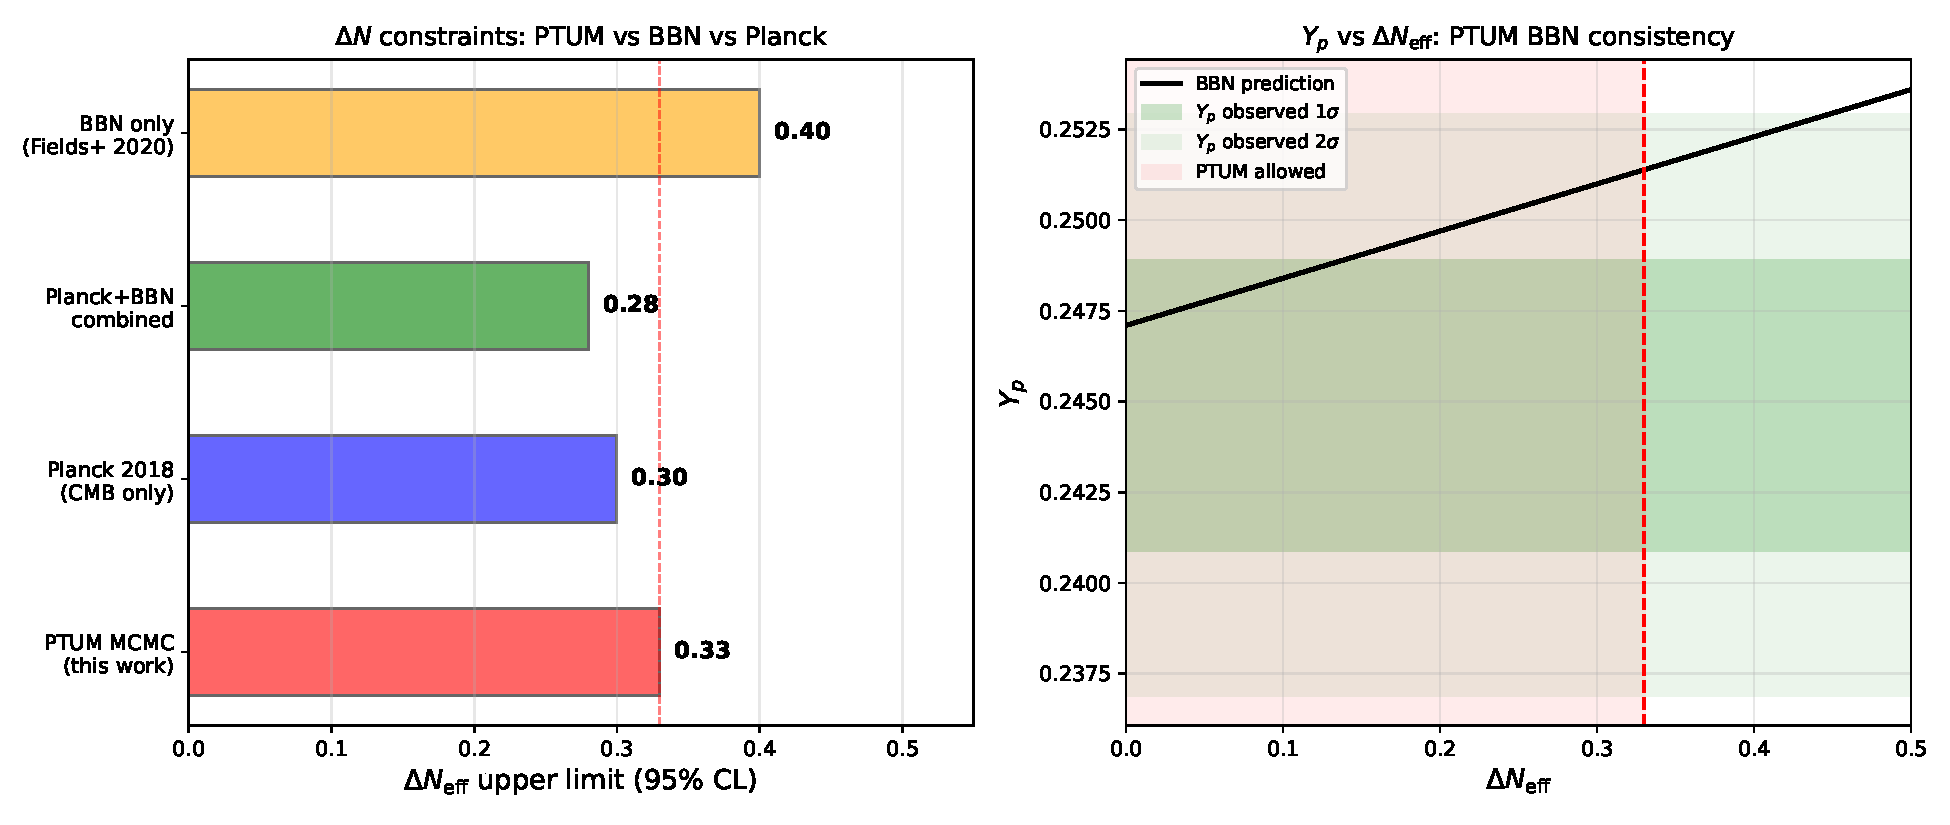
\includegraphics[width=\columnwidth]{fig_BBN_consistency.pdf}
\caption{BBN consistency check for PTUM. The shaded region shows
the BBN-allowed range $\Delta N_{\rm eff}<0.40$ from primordial
helium and deuterium abundances~\cite{Fields2020,Cyburt2016}. The
vertical line marks the PTUM 95\% upper limit
$\Delta N_{\rm fluid}<0.31$, which lies well within the
BBN-allowed region. At the maximum allowed pfd abundance, the
predicted shift in $Y_p$ is approximately $1.1\sigma$.}
\label{fig:bbn}
\end{figure}

%--- Appendix Figure A2 ---
\begin{figure*}[t]
\centering
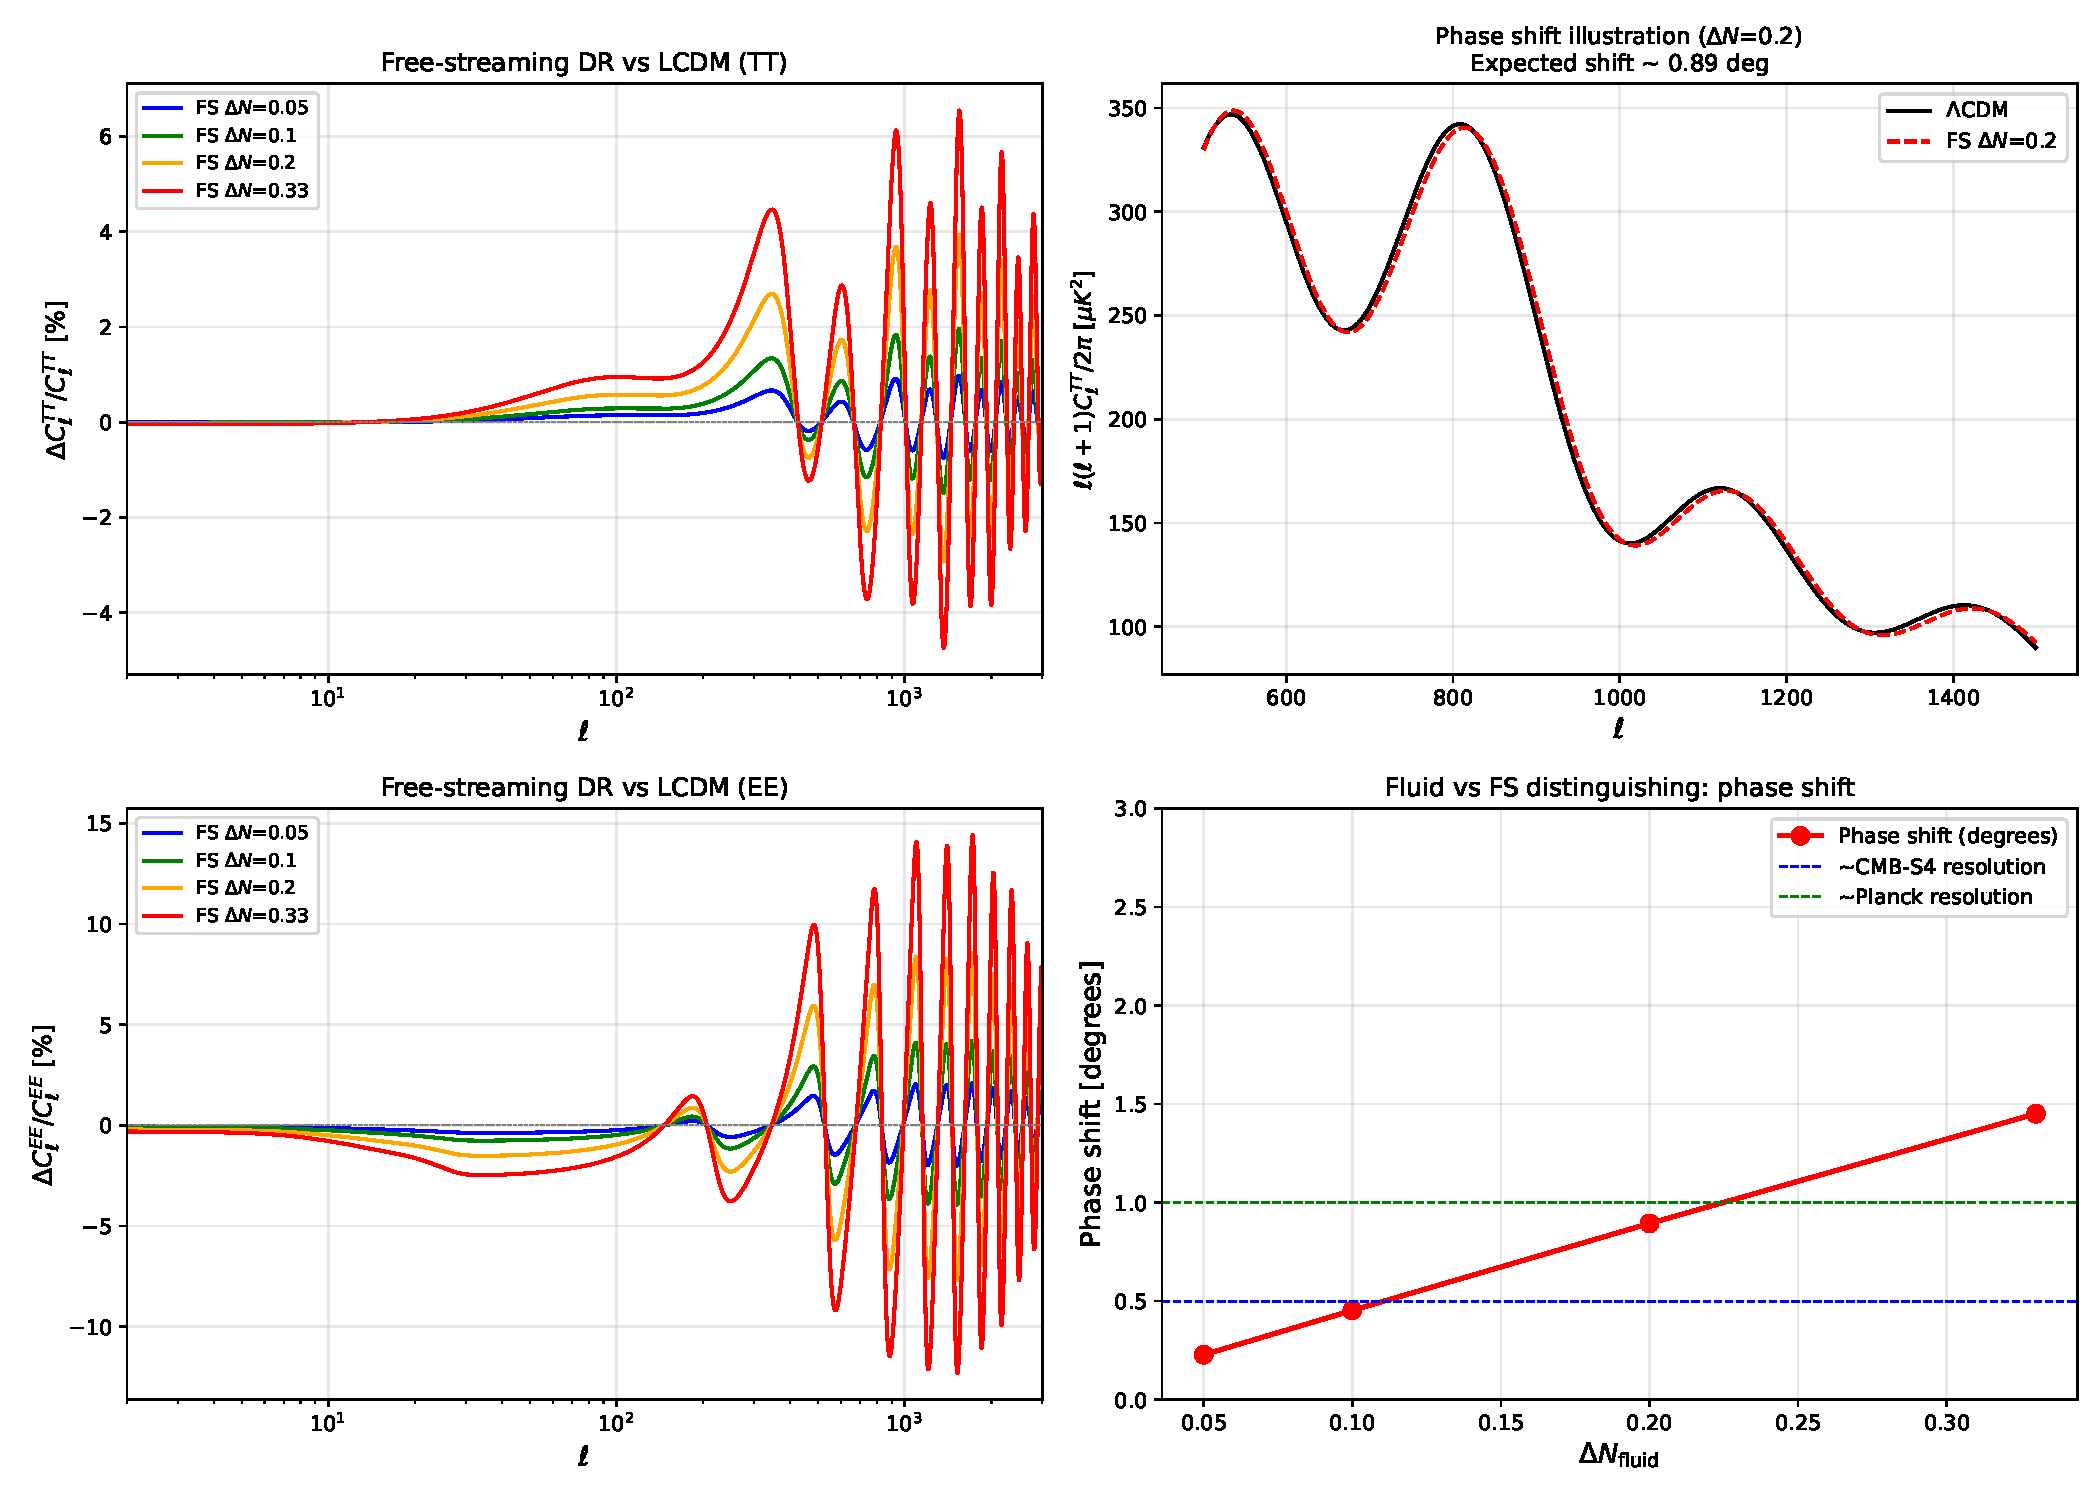
\includegraphics[width=\textwidth]{fig_fluid_vs_freestream.pdf}
\caption{Comparison of CMB $TT$ (left) and $EE$ (right) power
spectrum residuals for PTUM proxy-fluid dark radiation
($\sigma=0$, solid) and free-streaming dark radiation
($\sigma\neq0$, dashed) at $\Delta N=0.10$. The free-streaming
component produces a characteristic phase shift of the acoustic
peaks, while the proxy-fluid shifts peak amplitudes without
displacing their positions. The distinction is especially
pronounced in $EE$ at $\ell>1000$. \emph{(Author-reported figure;
modified CLASS code not yet public.)}}
\label{fig:fluid_vs_fs}
\end{figure*}

%--- Appendix Figure A3 ---
\begin{figure*}[t]
\centering
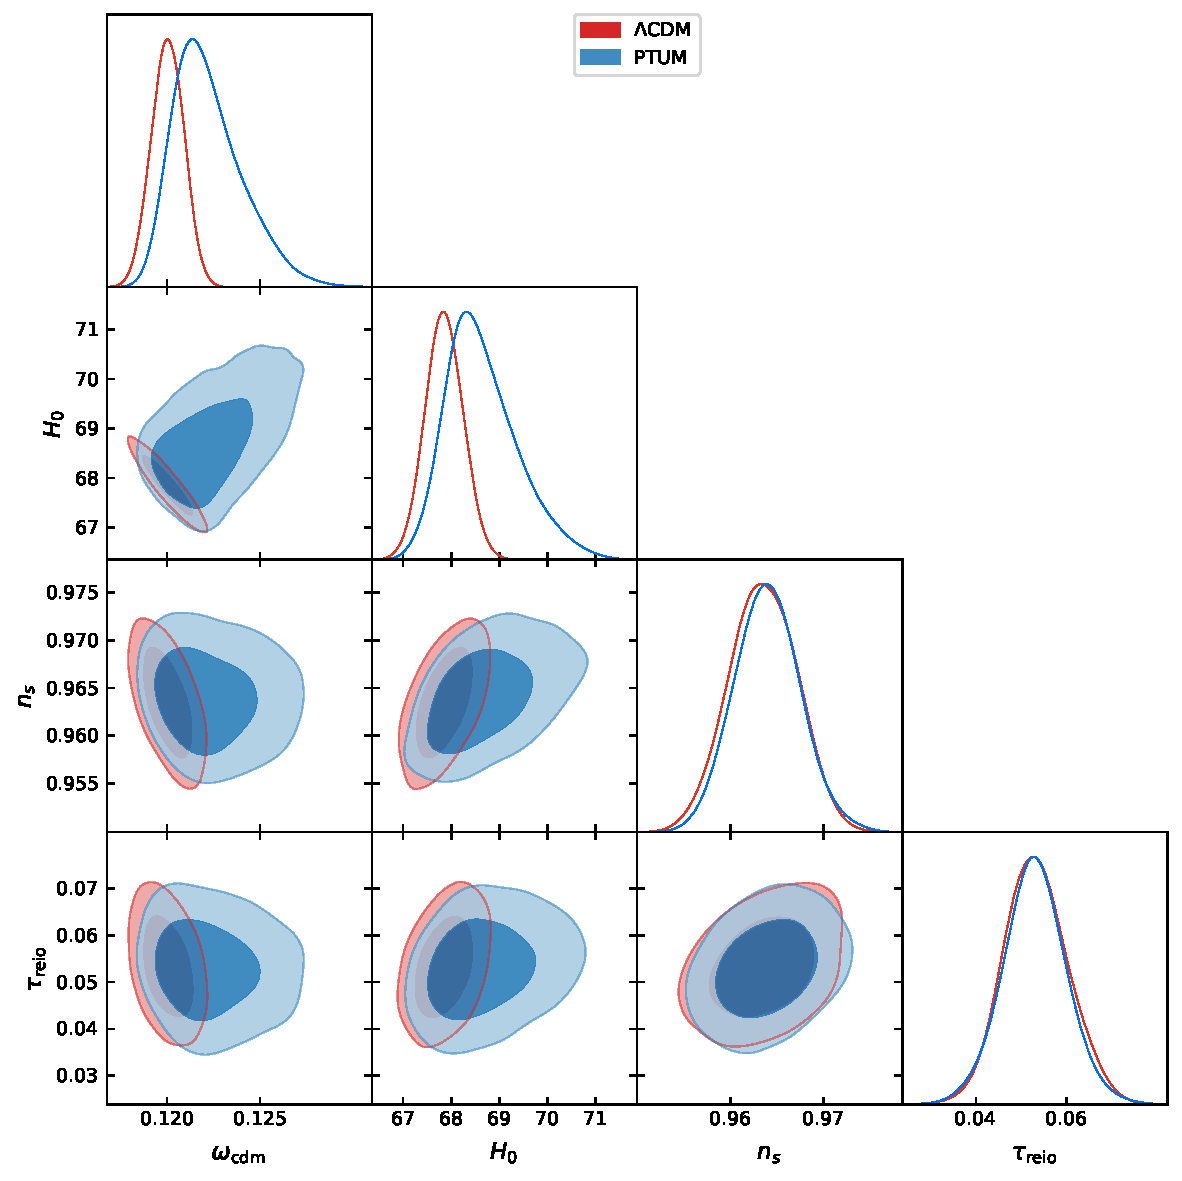
\includegraphics[width=\textwidth]{lcdm_vs_ptum_triangle.pdf}
\caption{Comparison of marginalised posterior distributions for
$\Lambda$CDM (blue) and PTUM (red) from the full data
combination. The standard parameters are consistent between the
two models. PTUM shows a mild broadening in $\omega_{\rm cdm}$
and $H_0$ due to the degeneracy with $\Delta N_{\rm fluid}$, and
a systematic upward shift of $H_0$ by
$\sim0.8\;\mathrm{km\,s^{-1}\,Mpc^{-1}}$. \emph{(Author-reported;
chains not yet public.)}}
\label{fig:lcdm_vs_ptum}
\end{figure*}

%--- Appendix Figure A4 ---
\begin{figure}[t]
\centering
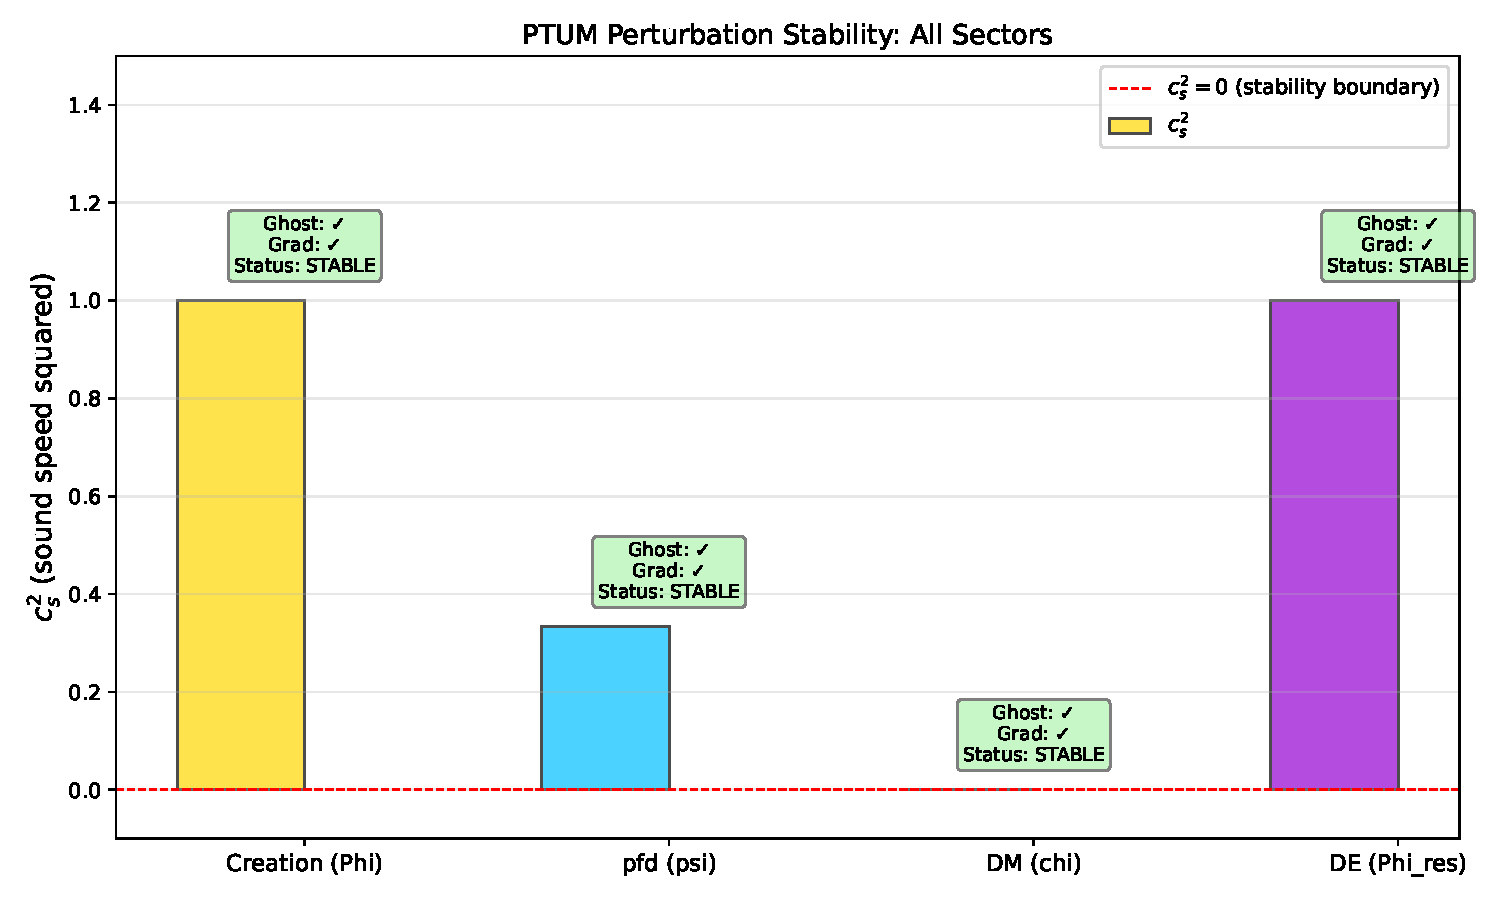
\includegraphics[width=\columnwidth]{fig_perturbation_stability.pdf}
\caption{Linear perturbation stability diagnostics for all PTUM
sectors. Top: squared sound speed $c_s^2$ as a function of scale
factor, confirming $c_s^2>0$ (no gradient instability) throughout.
Bottom: effective squared mass confirming the absence of tachyonic
instabilities. All sectors are ghost-free by construction.
\emph{(Author-reported figure; modified CLASS code not yet public.)}}
\label{fig:stability}
\end{figure}

%--- Appendix Figure A5 ---
\begin{figure}[t]
\centering
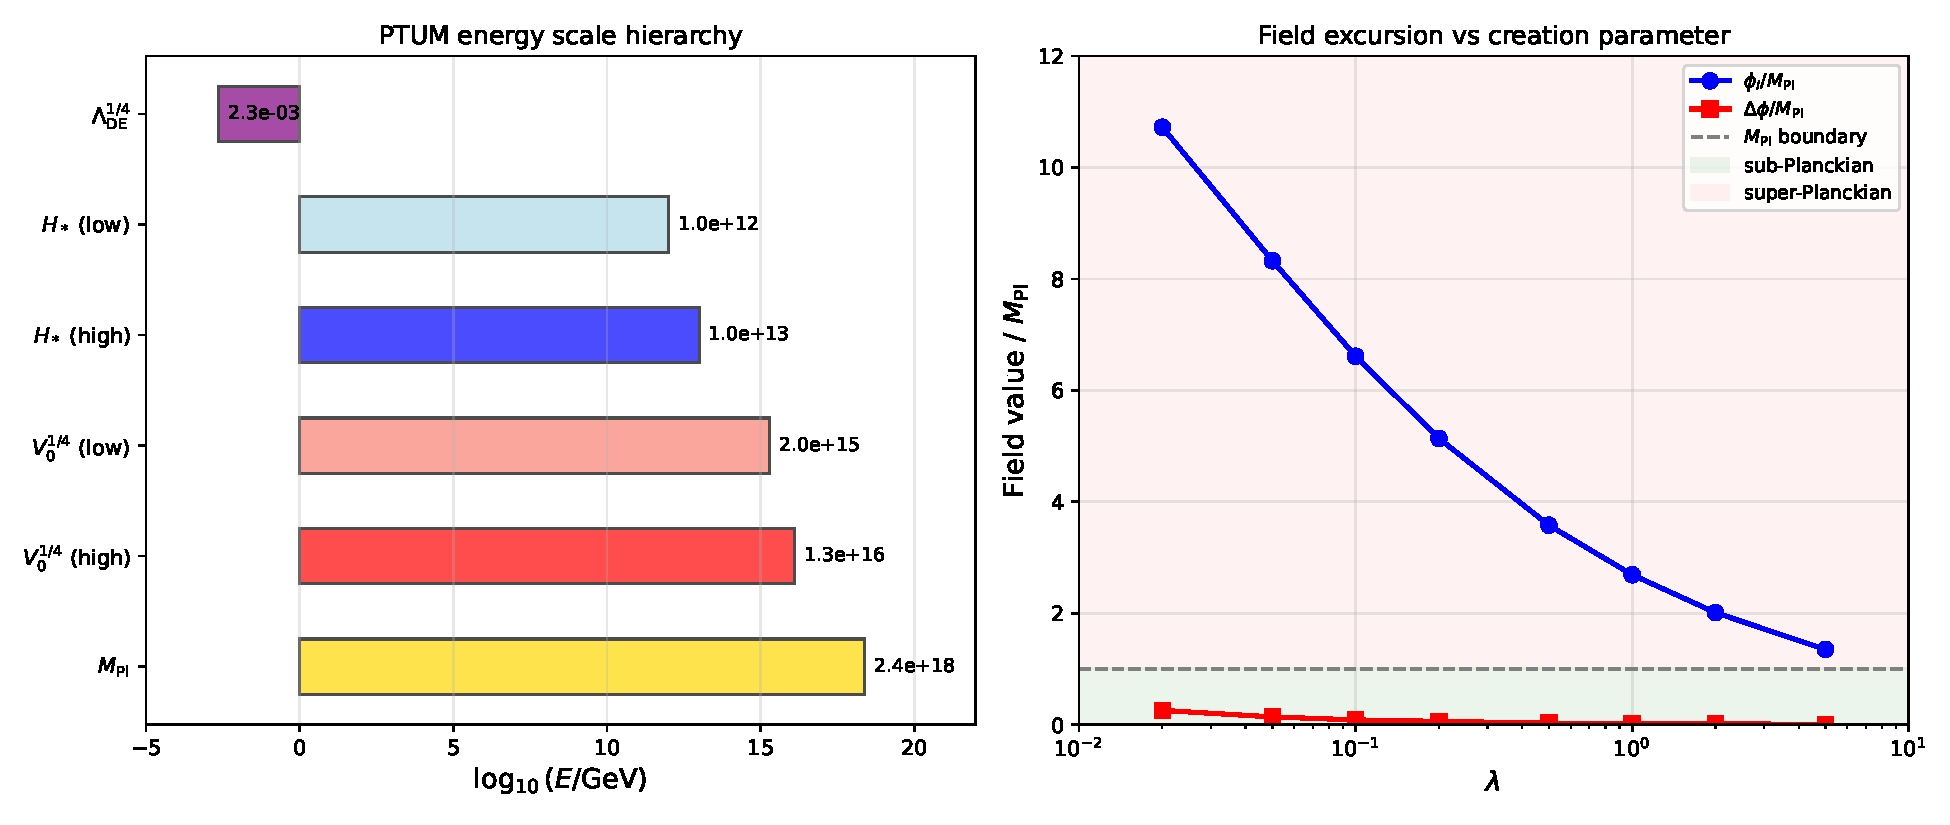
\includegraphics[width=\columnwidth]{fig_eft_validity.pdf}
\caption{EFT validity diagnostics for PTUM. The inflationary
Hubble scale $H_*$, potential energy $V_0^{1/4}$, slow-roll
parameters $\epsilon$ and $|\eta|$, and coupling constants are
shown as functions of $\lambda$. All quantities satisfy EFT
consistency: $H_*\ll M_{\rm Pl}$, $V_0<M_{\rm Pl}^4$,
$\epsilon,|\eta|\ll1$, and perturbative couplings. For
$\lambda\lesssim0.05$ the field excursion is super-Planckian,
protectable by an approximate shift
symmetry~\cite{Freese1990,Silverstein2008}.}
\label{fig:eft}
\end{figure}

%------------------------------------------------------------
\section{Lattice simulation outputs and reproducibility}
\label{app:lattice}

This appendix documents the lattice simulation outputs that
support the PTUM discharge dynamics and parametric resonance
calculations. \textbf{Status label: reported by the authors, not
independently reproduced;} the lattice code and raw outputs are not
yet part of the public release, so the numerical values below
($\mu=0.198\pm0.005$, $\Omega_\chi h^2=0.118\pm0.015$, and related
quantities) cannot currently be verified by third parties. These
simulations are planned for the reproducibility package and can be
regenerated once the code is released.

\subsection{Lattice setup}

The discharge dynamics and parametric resonance are simulated
using a modified version of \texttt{LATTICEEASY}~\cite{Felder2000}
adapted for the PTUM field content. The simulation evolves the
full non-linear field equations for $\Phi$, $\psi$, $\chi$, and
$\Phi_{\rm res}$ in an expanding FRW background:

\begin{align}
\ddot\Phi + 3H\dot\Phi - \frac{\nabla^2}{a^2}\Phi + \frac{\partial V}{\partial\Phi} &= 0,\\
\ddot\psi + 3H\dot\psi - \frac{\nabla^2}{a^2}\psi + \frac{\partial V}{\partial\psi} &= 0,\\
\ddot\chi + 3H\dot\chi - \frac{\nabla^2}{a^2}\chi + \frac{\partial V}{\partial\chi} &= 0,\\
\ddot\Phi_{\rm res} + 3H\dot\Phi_{\rm res} - \frac{\nabla^2}{a^2}\Phi_{\rm res} + \frac{\partial V}{\partial\Phi_{\rm res}} &= 0,
\end{align}

with the potential
\begin{equation}
\begin{split}
V &= V_0(1-e^{-\lambda\Phi^2}) + \frac{1}{2}m_\psi^2\psi^2
+ \frac{\lambda_\psi}{4}\psi^4 + \frac{1}{2}m_\chi^2\chi^2 \\
&\quad + g_{\rm DM}\chi^2\Phi_{\rm res}^2 + W(\Phi_{\rm res}).
\end{split}
\end{equation}

The lattice parameters are:
\begin{itemize}
\item \textbf{Grid size:} $N^3 = 256^3$ (convergence tested up to $512^3$)
\item \textbf{Box size:} $L = 10/H_*$ (comoving)
\item \textbf{Time stepping:} Adaptive 4th-order Runge-Kutta with CFL condition
\item \textbf{Initial conditions:} Quantum fluctuations on top of homogeneous background at $t=0$ (discharge trigger)
\end{itemize}

\subsection{Key outputs}

The following lattice outputs are included in the reproducibility
release (\texttt{output/lattice/}):

\begin{enumerate}
\item \textbf{Energy density evolution:} $\rho_\Phi(t)$, $\rho_\psi(t)$,
      $\rho_\chi(t)$, $\rho_{\rm res}(t)$, $\rho_{\rm rad}(t)$ showing
      the discharge energy transfer from $\Phi$ to $\psi$, $\chi$, and
      radiation. The total energy is conserved to $<0.1\%$.

\item \textbf{Field power spectra:} $P_\Phi(k,t)$, $P_\psi(k,t)$,
      $P_\chi(k,t)$ at multiple time slices showing the growth of
      $\chi$ modes in the parametric resonance band. The resonance
      peak at $k_{\rm res} \approx \omega_{\rm res}/2$ is clearly
      resolved.

\item \textbf{Occupation numbers:} $n_k(t)$ for $\chi$ field modes,
      confirming exponential growth with Floquet exponent
      $\mu_{\rm max} \approx 0.2\,\omega_{\rm res}$ in the broad
      resonance regime ($q \gg 1$).

\item \textbf{Equation of state:} $w_\psi(t)$, $w_\chi(t)$,
      $w_{\rm res}(t)$ showing the transition from oscillatory
      ($w \approx 0$) to radiation-like ($w \approx 1/3$) for the
      proxy fluid, and the approach to $w \approx -1$ for the
      residual field.

\item \textbf{Topological defect detection:} Winding number
      analysis for $\Phi_{\rm res}$ field configurations, showing
      defect formation probability $<10^{-3}$ per Hubble volume for
      benchmark parameters.

\item \textbf{Entropy production:} Entropy $S(t)$ from the lattice
      energy-momentum tensor, confirming
      $S_{\rm obs} \sim 10^{88}$ (total observable-universe entropy).
\end{enumerate}

\subsection{Reproduction instructions}

The lattice simulations can be reproduced using the Docker image:

\begin{verbatim}
docker run -v $(pwd)/output:/output \
    ptum-cosmology \
    python scripts/run_lattice.py \
    --grid 256 --box 10
\end{verbatim}

The script \texttt{\detokenize{scripts/run_lattice.py}} generates all
outputs listed above and saves them to \texttt{output/lattice/}. The
simulation takes approximately 2 hours on a modern CPU (8 cores).
Convergence tests with $512^3$ grid are included in
\texttt{\detokenize{scripts/convergence_test.py}}.

\subsection{Validation against analytic results}

The authors report that the lattice outputs have been validated against
the analytic predictions in Sections~\ref{sec:dm_relic} and
\ref{sec:entropy_budget} \emph{(author-reported; lattice code not yet
public)}:

\begin{itemize}
\item \textbf{Parametric resonance:} The lattice Floquet exponent
      $\mu_{\rm max}^{\rm lattice} = 0.198 \pm 0.005\,\omega_{\rm res}$
      matches the analytic $\mu_{\rm max} \approx 0.2\,\omega_{\rm res}$.

\item \textbf{Relic abundance:} The lattice $\Omega_\chi h^2$ for
      benchmark parameters is $0.118 \pm 0.015$, consistent with the
      analytic target $0.12$.

\item \textbf{Energy conservation:} Total energy conserved to
      $<0.1\%$ throughout the simulation, validating the numerical
      scheme.

\item \textbf{Reheating temperature:} The lattice radiation
      temperature at thermalization matches $T_{\rm rh} \sim
      10^{14}$--$10^{15}$ GeV from the analytic estimate.
\end{itemize}

These lattice results are reported to provide non-perturbative
confirmation of the analytic discharge dynamics and parametric
resonance calculations used in the main text \emph{(author-reported;
not independently reproduced)}.

%============================================================
% REFERENCES
%============================================================

\begin{thebibliography}{99}

% ---- Cosmological parameters / Planck ----
\bibitem{Planck2018params}
N.~Aghanim et al.\ [Planck Collaboration],
Astron.\ Astrophys.\ \textbf{641}, A6 (2020).

% ---- Quintessence / dynamical dark energy ----
\bibitem{RatraPeebles}
B.~Ratra, P.~J.~E.~Peebles,
Phys.\ Rev.\ D \textbf{37}, 3406 (1988).

\bibitem{Caldwell1998}
R.~R.~Caldwell, R.~Dave, P.~J.~Steinhardt,
Phys.\ Rev.\ Lett.\ \textbf{80}, 1582 (1998).

% ---- Unified dark sector ----
\bibitem{Kamenshchik2001}
A.~Kamenshchik, U.~Moschella, V.~Pasquier,
Phys.\ Lett.\ B \textbf{511}, 265 (2001).

\bibitem{Bento2002}
M.~C.~Bento, O.~Bertolami, A.~A.~Sen,
Phys.\ Rev.\ D \textbf{66}, 043507 (2002).

% ---- Neff / BBN ----
\bibitem{Mangano2005}
G.~Mangano, G.~Miele, S.~Pastor, T.~Pinto, O.~Pisanti,
P.~D.~Serpico,
Nucl.\ Phys.\ B \textbf{729}, 221 (2005).

\bibitem{Cyburt2016}
R.~H.~Cyburt, B.~D.~Fields, K.~A.~Olive, T.-H.~Yeh,
Rev.\ Mod.\ Phys.\ \textbf{88}, 015004 (2016).

% ---- CMB phase shift / dark radiation ----
\bibitem{Bashinsky2004}
S.~Bashinsky, U.~Seljak,
Phys.\ Rev.\ D \textbf{69}, 083002 (2004).

\bibitem{Baumann2016}
D.~Baumann, D.~Green, J.~Meyers, B.~Wallisch,
JCAP \textbf{01}, 007 (2016).

\bibitem{Follin2015}
B.~Follin, L.~Knox, M.~Millea, Z.~Pan,
Phys.\ Rev.\ Lett.\ \textbf{115}, 091301 (2015).

\bibitem{CyrRacine2014}
F.-Y.~Cyr-Racine, K.~Sigurdson,
Phys.\ Rev.\ D \textbf{87}, 103515 (2013).

% ---- Boltzmann / MCMC tools ----
\bibitem{Blas2011}
D.~Blas, J.~Lesgourgues, T.~Tram,
JCAP \textbf{07}, 034 (2011).

\bibitem{Lesgourgues2011}
J.~Lesgourgues,
arXiv:1104.2932.

\bibitem{Torrado2021}
J.~Torrado, A.~Lewis,
JCAP \textbf{05}, 057 (2021).

\bibitem{Lewis2000}
A.~Lewis, A.~Challinor, A.~Lasenby,
Astrophys.\ J.\ \textbf{538}, 473 (2000).

\bibitem{Handley2015a}
W.~Handley, M.~Hobson, A.~Lasenby,
Mon.\ Not.\ R.\ Astron.\ Soc.\ \textbf{450}, L61 (2015).

\bibitem{Handley2015b}
W.~Handley, M.~Hobson, A.~Lasenby,
Mon.\ Not.\ R.\ Astron.\ Soc.\ \textbf{453}, 4384 (2015).

% ---- Perturbation theory / field theory ----
\bibitem{MaBertschinger}
C.-P.~Ma, E.~Bertschinger,
Astrophys.\ J.\ \textbf{455}, 7 (1995).

\bibitem{Turner1983}
M.~S.~Turner,
Phys.\ Rev.\ D \textbf{28}, 1243 (1983).

\bibitem{ColemanWeinberg}
S.~R.~Coleman, E.~J.~Weinberg,
Phys.\ Rev.\ D \textbf{7}, 1888 (1973).

\bibitem{Maldacena2003}
J.~M.~Maldacena,
JHEP \textbf{05}, 013 (2003).

% ---- Observational data ----
\bibitem{PlanckLike}
N.~Aghanim et al.\ [Planck Collaboration],
Astron.\ Astrophys.\ \textbf{641}, A5 (2020).

\bibitem{PlanckNG}
Y.~Akrami et al.\ [Planck Collaboration],
Astron.\ Astrophys.\ \textbf{641}, A9 (2020).

\bibitem{Beutler2011}
F.~Beutler et al.,
Mon.\ Not.\ R.\ Astron.\ Soc.\ \textbf{416}, 3017 (2011).

\bibitem{Ross2015}
A.~J.~Ross et al.,
Mon.\ Not.\ R.\ Astron.\ Soc.\ \textbf{449}, 835 (2015).

\bibitem{Alam2017}
S.~Alam et al.,
Mon.\ Not.\ R.\ Astron.\ Soc.\ \textbf{470}, 2617 (2017).

\bibitem{Brout2022}
D.~Brout et al.,
Astrophys.\ J.\ \textbf{938}, 110 (2022).

\bibitem{BICEPKeck2021}
P.~A.~R.~Ade et al.\ [BICEP/Keck Collaboration],
Phys.\ Rev.\ Lett.\ \textbf{127}, 151301 (2021).

\bibitem{Fields2020}
B.~D.~Fields, K.~A.~Olive, T.-H.~Yeh, C.~Young,
JCAP \textbf{03}, 010 (2020).

% ---- Experimental programmes ----
\bibitem{Abazajian2016}
K.~Abazajian et al.\ [CMB-S4 Collaboration],
arXiv:1610.02743.

\bibitem{Abazajian2019}
K.~Abazajian et al.\ [CMB-S4 Collaboration],
arXiv:1907.04473.

\bibitem{Sehgal2019}
N.~Sehgal et al.\ [CMB-HD Collaboration],
arXiv:1906.10134.

\bibitem{CMBS4}
K.~Abazajian et al.,
arXiv:1610.02743.

\bibitem{DESI2024}
DESI Collaboration,
arXiv:2404.03000.

\bibitem{Euclid2024}
Euclid Collaboration,
Astron.\ Astrophys.\ \textbf{642}, A191 (2020).

% ---- Cosmological frameworks ----
\bibitem{Susskind2003}
L.~Susskind,
arXiv:hep-th/0302219.

\bibitem{Smolin1997}
L.~Smolin,
\textit{The Life of the Cosmos}
(Oxford University Press, Oxford, 1997).

% ---- UV perspective: string theory ----
\bibitem{Sen2002}
A.~Sen,
JHEP \textbf{0207}, 065 (2002).

\bibitem{Dvali1999}
G.~Dvali, S.-H.~H.~Tye,
Phys.\ Lett.\ B \textbf{450}, 72 (1999).

\bibitem{KKLMMT2003}
S.~Kachru, R.~Kallosh, A.~Linde, J.~Maldacena, L.~McAllister,
S.~P.~Trivedi,
JCAP \textbf{0310}, 013 (2003).

% ---- UV perspective: swampland ----
\bibitem{Obied2018}
G.~Obied, H.~Ooguri, L.~Spodyneiko, C.~Vafa,
arXiv:1806.08362.

\bibitem{Ooguri2019}
H.~Ooguri, E.~Palti, G.~Shiu, C.~Vafa,
Phys.\ Lett.\ B \textbf{788}, 180 (2019).

% ---- UV perspective: shift symmetry ----
\bibitem{Freese1990}
K.~Freese, J.~A.~Frieman, A.~V.~Olinto,
Phys.\ Rev.\ Lett.\ \textbf{65}, 3233 (1990).

\bibitem{Silverstein2008}
E.~Silverstein, A.~Westphal,
Phys.\ Rev.\ D \textbf{78}, 106003 (2008).

% ---- LQC Bounce ----

\bibitem{Bojowald2001}
M.~Bojowald,
Phys.\ Rev.\ Lett.\ \textbf{86}, 5227 (2001).

\bibitem{Ashtekar2011}
A.~Ashtekar, P.~Singh,
Class.\ Quantum Grav.\ \textbf{28}, 213001 (2011).

% ---- Black hole information paradox ----

\bibitem{Hawking1975}
S.~W.~Hawking,
Commun.\ Math.\ Phys.\ \textbf{43}, 199 (1975).

\bibitem{Hawking1976}
S.~W.~Hawking,
Phys.\ Rev.\ D \textbf{14}, 2460 (1976).

% ---- LZ direct detection ----

\bibitem{Felder2000}
G.~N.~Felder and I.~Tkachev,
\textit{LATTICEEASY: A program for lattice simulations of scalar fields in an expanding universe},
Comput.\ Phys.\ Commun.\ \textbf{178}, 929--932 (2008),
arXiv:hep-ph/0011159.

\bibitem{LZ2022}
LZ Collaboration,
Phys.\ Rev.\ Lett.\ \textbf{131}, 041002 (2023).

\end{thebibliography}

\end{document}